% Below is your UAH LaTeX template. This is the main file that compiles your document. You will need to fill out the appropriate sections below.
\documentclass[oneside, 12pt]{book} % Document class


\usepackage[utf8]{inputenc} % Basic package for Latex
%\usepackage[draft]{graphicx} % To help include figures
\usepackage{listings}
\lstset{basicstyle=\ttfamily}
\usepackage{graphicx} % To help include figures
\usepackage{geometry} % To allow document margin changes
\usepackage{setspace} % To allow custom spacing
\usepackage{indentfirst} % To allow indentations in the first paragraph.
\usepackage{amsmath} % For formatting equations properly
\usepackage{natbib} % For formatting the bibliography
\usepackage{chngcntr} % To allow changing how figures, tables, and pages are counted.
\usepackage{appendix} % To help format the appendix
\usepackage[font=small,labelfont=bf]{caption} %This makes caption font small and makes the caption heading bold.
\usepackage{tabularx} %To allow formatting Tables.
\usepackage{array} %To allow creating arrays.
\usepackage{multirow, tabularx}
\usepackage{multicol}
\usepackage{physics}
\providecommand\phantomsection{} %This command allows you to make phantom sections that have no title but are still included in the Table of Contents such as the epigraph.
\usepackage[all]{nowidow} %This prevents widow/orphan lines
\usepackage{tikz}%This package helps to anchor the seal on the title page to the student name
\usetikzlibrary{tikzmark}%This is part of the tikz package


%Creating an Interlude Environment in order to NOT count or number a certain page such as the copyright page.
\newenvironment{interlude}{
  \clearpage
  \thispagestyle{empty}% we want this page to be empty (adjust to use a modified page style)
  \pagestyle{empty}% use the same style for subsequent pages in the unnumbered section
  }
  {\clearpage}

%The following package and lines can be used to format and create a list of symbols, equations, abbreviations, etc. The example actually used in this template is the \glossaries package, but you may also use this \nomencl package if desired.
\usepackage[intoc]{nomencl}
\makenomenclature
\renewcommand{\nomname}{List of Symbols}

% This is to ensure the page numbers are centered and at the bottom.
\usepackage{fancyhdr}
\pagestyle{fancy}
\fancyhf{}
\renewcommand{\headrulewidth}{0pt}
\cfoot{\thepage}

%This defines a new page style for just the title page.
\fancypagestyle{logopage}{\fancyhf{}\renewcommand{\headrulewidth}{0pt}\fancyfoot[C]{\includegraphics[scale=0.3]{Figures/Color Grad Banner.png}}}

%this causes equations to be counted according to their chapter location
\counterwithin{equation}{chapter} %this causes equations to be counted according to their chapter location
\counterwithin{figure}{chapter}




%This formats the table of contents the way Dr. Hakkila wants it
\usepackage[titles]{tocloft}


%Removes the Duplicate Chapter
\setcounter{secnumdepth}{4}% Show down to subsubsection

\setlength{\cftchapindent}{-20pt}% Just some value...

\usepackage{xpatch}

\makeatletter
\xpatchcmd{\@chapter}{\addcontentsline{toc}{chapter}{\protect\numberline{\thechapter}#1}}{%
                      \addcontentsline{toc}{chapter}{\protect\numberline{}#1}}{\typeout{Success}}{\typeout{Failed!}}
\makeatother



%This formats the Table of contents title
\renewcommand{\contentsname}{\hspace*{\fill}\bfseries\large Table of Contents\hspace*{\fill}}


\renewcommand{\cftbeforetoctitleskip}{-0.25in}

\renewcommand\cftchapdotsep{\cftdotsep}
\renewcommand\cftchapleader{\cftdotfill{\cftchapdotsep}}
%\renewcommand{\cftchappresnum}{CHAPTER } % put this before the number
%\addtolength{\cftchapnumwidth}{6em} % extra space for number and pre-name
%\renewcommand{\cftchapaftersnum}{. } % put period after chapter number and space


%This puts all the chapter headings into all-caps
%\renewcommand{\chaptername}{CHAPTER}

%Hopefully this reformats the List of Figures Title
\renewcommand{\listfigurename}{\hspace*{\fill}\bfseries\large List of Figures\hspace*{\fill}}

%Reformat List of Tables, etc.
\renewcommand{\listtablename}{\hspace*{\fill}\bfseries\large List of Tables\hspace*{\fill}}


%This creates a List of Equations.
\newcommand{\listequationsname}{List of Equations}
\newlistof{equations}{equ}{\listequationsname}

\newcommand{\eqdesc}[1]{%
  \csname phantomsection\endcsname % if hyperref is loaded
  \addcontentsline{equ}{equations}{\protect\numberline{\theequation}#1}%
}

\setlength{\parindent}{36pt}


%The following formats the chapter titles and sections appropriately
\usepackage{titlesec}



\titleformat
{\chapter}
[hang]
{\normalfont\large\bfseries\filcenter}
{} %Label. This is blank so that the entire chapter heading and title are properly centered.
{0pt} %  Horizontal Space between label and title body.
{} %Before-Code
{}

\titleformat
{\section}
[hang]
{\normalfont\normalsize\bfseries}
{\thetitle} %Label.
{.5em} %  Horizontal Space between label and title body.
{} %Before-Code
{}

\titleformat
{\subsection}
[hang]
{\normalfont\normalsize\bfseries}
{\thetitle} %Label.
{.5em} %  Horizontal Space between label and title body.
{} %Before-Code
{}

\titlespacing{\subsection}{2em}{12pt}{12pt}

\titlespacing{\chapter}{0pt}{50pt}{12pt}

\titlespacing{\part}{0pt}{12pt}{12pt}


\titlespacing{name=\chapter, numberless}{0pt}{0pt}{12pt}


% I had used this code to combine the chapter heading and
%\titleformat{\chapter}[hang]
 % {\normalfont\large\bfseries\filcenter}{\chaptertitlename\ \thechapter:}{.3em}{}


%This names the Bibliography/References whatever you want it to be.
\renewcommand{\bibname}{References}

%The below package creates the optional List of Symbols and formats it correction..
\usepackage[acronyms, automake, toc, nopostdot]{glossaries}
\usepackage{glossary-longbooktabs}
\newcolumntype{P}[1]{>{\centering\arraybackslash}p{#1}}
\renewcommand*{\entryname}{Symbol}
\newglossarystyle{mystyle}{% define custom glossaries style for Abbreviation page, read relative manual before change
\setglossarystyle{long-booktabs}%
\renewenvironment{theglossary}%
{\begin{longtable}{@{}P{3cm}@{}p{\dimexpr\linewidth-3cm}@{}}}%
{\end{longtable}}%

\renewcommand*{\glossaryheader}{%
 \bfseries\large Symbol & \centering\bfseries\large Description \tabularnewline\endhead \endfoot}%
}

\renewcommand{\glossarypreamble}{\normalsize}
\makeglossaries
 %To clean up this document, the preamble that includes the packages is located in the preamble.tex file found in the FrontMatter folder.

%********************************************
%********************************************
% THE SECTION BELOW MUST BE FILLED OUT
%********************************************
%********************************************

%BASIC INFORMATION
\newcommand{\thesistitle}{Deep Learning Time Series Prediction Strategies for Efficiently Emulating Noah Land Surface Model Soil Moisture Dynamics}
\newcommand{\studentname}{Mitchell T. Dodson}
\newcommand{\degree}{Master of Science in Atmospheric Science}
\newcommand{\department}{Atmospheric and Earth Science}
\newcommand{\gradyear}{2025}% complete 4 digit year, e.g., 2022
\newcommand{\gradmonth}{May}% Spell out the month completely, e.g., December
%\newcommand{\jointuni}{Auburn University} %If this is a joint degree, remove the % sign at the beginning of this line and enter the entire name of the additional universities.

%***********************
%SPECIFY THESIS OR DISSERTATION
% Below, if you are earning a master's degree, remove the "%" on the line below that says \newcommand{thesis}. If you are earning a PhD or other doctorate degree, remove the "%" on the line below that says \newcommand{dissertation}.

\newcommand{\thesis}{FOR MASTER'S STUDENTS ONLY}
%\newcommand{\dissertation}{FOR DOCTORATE DEGREE STUDENTS ONLY}

%*******************************
%SPECIFY THE PROFESSORS WHO WILL APPROVE YOUR THESIS/DISSERTATION
%Professor information: Fill out only their first and last name WITH NO PREFIXES OR SUFFIXES. If a line is not applicable, simply add a % sign at the beginning of that line. If there is an applicable line that has a % sign at the beginning, remove this sign and fill in as needed.
\newcommand{\resadv}{Christopher Hain}
\newcommand{\comchair}{Sundar Christopher}
%\newcommand{\reschair}{Research Advisor/Committee Chair Name} %If your research advisor and committee chair are the same person, enter his/her name on this line.
\newcommand{\commema}{Sean Freeman}
%\newcommand{\commemb}{[2nd Committee Member Name]}
%\newcommand{\commemc}{[3rd Committee Member Name]}
%\newcommand{\commemd}{[4th Committee Member Name]}
%\newcommand{\commeme}{[5th Committee Member Name]}
%\newcommand{\commemf}{[6th Committee Member Name]}
%\newcommand{\commemg}{[7th Committee Member Name]}
%\newcommand{\commemh}{[8th Committee Member Name]}
%\newcommand{\commemi}{[9th Committee Member Name]}
\newcommand{\depchair}{Lawrence Carey}
\newcommand{\colldean}{[Rainer Steinwandt]}
\newcommand{\graddean}{Jon Hakkila}

%**************
%INDICATE IF YOU HAVE REGISTERED FOR A COPYRIGHT.
%**************
%\newcommand{\copyrightreg}{Yes} %If you registered for a copyright through Proquest, please remove the % sign from the beginning of this line starting with \newcommand{\copyrightreg}{Yes}. If you did not register for a copyright, no action is needed.

%********************************************
%********************************************
% End of Section to Fill Out.
%********************************************
%********************************************

%This creates hyperlinks for chapter, figure, and table titles in your pdf. It should be the last package before the document begins.
\usepackage[colorlinks=true,linkcolor=black,anchorcolor=black,citecolor=black,filecolor=black,menucolor=black,runcolor=black,urlcolor=black]{hyperref}

%*********************************************
%*********************************************
%Optional List of Symbols/Abbreviations
%*********************************************
%*********************************************

%A list of symbols/abbreviations is optional. If you do not want to include one, simply delete this section from your document. You may also delete this section and use a different package as there are multiple packages that can be used to make a List of Symbols, Abbreviations, Nomenclature, Etc. Below uses the \glossaries-extra package. This package is nice if you want to include multiple lists or sections. The following links provide useful information on how to use this package.
% https://mirrors.mit.edu/CTAN/macros/latex/contrib/glossaries/glossariesbegin.pdf
% https://mirrors.rit.edu/CTAN/macros/latex/contrib/glossaries/glossaries-user.pdf
% https://www.overleaf.com/learn/latex/Glossaries


% This uses the glossaries package. With this package, you can include multiple types of lists, track page numbers if desired, and define new lists. More information can be found at the following sites: https://mirrors.mit.edu/CTAN/macros/latex/contrib/glossaries/glossariesbegin.pdf and https://mirrors.rit.edu/CTAN/macros/latex/contrib/glossaries/glossaries-user.pdf https://www.overleaf.com/learn/latex/Glossaries


%*****************************************
%Define your list of glossary items below. Remember that the entries that you enter in this file will not automatically appear in the List of Symbols. You also have to reference the symbol in the body of your thesis by using the \gls command. 

%symbols
\newglossaryentry{deg}{name=$^\circ$, description={Degree}}
\newglossaryentry{grav}{name={1D}, description={Normal gravity environment}}
\newglossaryentry{wf}{name={\textit{f}}, description={Wear factor}}
\newglossaryentry{alp}{name={$\alpha$},description={Alpha}}
\newglossaryentry{theta}{name={$r_O$}, description={ecosystem respiration at reference temperature $T_a=0{^\circ}$C}}
\newglossaryentry{te}{name={$\tau_e$}, description={precision of the normal distribution of the likelihood}}
\newglossaryentry{q10}{name={$Q_{10}$}, description={multiplication factor to respiration with 10$^\circ$C increases in $T_a$}}
\newglossaryentry{phi}{name={$\phi$}, description={vapour pressure deficit response function}}
\newglossaryentry{del}{name=$\delta$, description={Transition coefficient constant for the design of linear-phase FIR filters which are used to take up space when testing the list of symbols}}

 %Go to this page to enter all the symbols you plan to use in the document.

% Scroll down in this file to after the List of Tables section in order to actually add your Lists to your document,.

%**********************************************
%**********************************************
% End of Optional List of Symbols/Abbreviations
%**********************************************
%**********************************************



%******************************************
%******************************************
% Document Begins Here
%******************************************
%******************************************

\begin{document}

\frontmatter % This command creates the front matter environment.

%**********************************
%**********************************
%Title Page
%**********************************
%**********************************
% Do not directly edit this page. Everything on the Title Page should auto-fill if you correctly filled out the information on the main.tex file.

\begin{titlepage}
\newgeometry{left=1.5in,bottom=.5in}
    \begin{center}
        \Large
        \singlespacing
        \textbf{\thesistitle}
        

\vspace{2cm}

        \large
        \textbf{\studentname}\\
        \vspace{1.5cm}
        \normalsize
        \ifdefined\thesis
        \textbf{A THESIS}
        \vspace{1.5cm}
        \else
        \ifdefined\dissertation
        \textbf{A DISSERTATION}
        \vspace{1.5cm}
        \else
        Please identify this document as either a thesis or dissertation on the main.tex file in the section at the top that must be filled out.
        \vspace{1.5cm}
        \fi
        \fi

        \textbf{Submitted in partial fulfillment of the requirements \\for the degree of \degree}\\  
        
\vspace{0.1cm}
  \textbf{in}\\
      \vspace{0.1cm}
        \textbf{The Department of \department}\\
        \vspace{0.1cm}
  \textbf{to}\\
\vspace{0.1cm}
\textbf{The Graduate School}\\
\vspace{0.1cm}
\textbf{of}\\
\vspace{0.1cm}
        \ifdefined\jointuni
        \textbf{The University of Alabama in Huntsville\\ and\\  \jointuni}
        \else
        \textbf{The University of Alabama in Huntsville}
    \fi

        
        \vspace{0.4cm}
        \textbf{\gradmonth\ \gradyear}
        


    \end{center}
    

\vfill

\textbf{Approved by:}


\vspace{.1cm}
\setstretch{1.25}

\ifdefined\reschair
\noindent
Dr. \reschair, Research Advisor/Committee Chair\\
\else
\noindent
Dr. \resadv, Research Advisor \\
Dr. \comchair, Committee Chair\\
\fi
\ifdefined\commemi
\noindent
Dr. \commema, Committee Member\\
Dr. \commemb, Committee Member\\
Dr. \commemc, Committee Member\\
Dr. \commemd, Committee Member\\
Dr. \commeme, Committee Member\\
Dr. \commemf, Committee Member\\
Dr. \commemg, Committee Member\\
Dr. \commemh, Committee Member\\
Dr. \commemi, Committee Member\\
Dr. \depchair, Department Chair\\
Dr. \colldean, College Dean\\
Dr. \graddean, Graduate Dean\\
\else
\ifdefined\commemh
\noindent
Dr. \commema, Committee Member\\
Dr. \commemb, Committee Member\\
Dr. \commemc, Committee Member\\
Dr. \commemd, Committee Member\\
Dr. \commeme, Committee Member\\
Dr. \commemf, Committee Member\\
Dr. \commemg, Committee Member\\
Dr. \commemh, Committee Member\\
Dr. \depchair, Department Chair\\
Dr. \colldean, College Dean\\
Dr. \graddean, Graduate Dean\\
\else
\ifdefined\commemg
\noindent
Dr. \commema, Committee Member\\
Dr. \commemb, Committee Member\\
Dr. \commemc, Committee Member\\
Dr. \commemd, Committee Member\\
Dr. \commeme, Committee Member\\
Dr. \commemf, Committee Member\\
Dr. \commemg, Committee Member\\
Dr. \depchair, Department Chair\\
Dr. \colldean, College Dean\\
Dr. \graddean, Graduate Dean\\
\else
\ifdefined\commemf
\noindent
Dr. \commema, Committee Member\\
Dr. \commemb, Committee Member\\
Dr. \commemc, Committee Member\\
Dr. \commemd, Committee Member\\
Dr. \commeme, Committee Member\\
Dr. \commemf, Committee Member\\
Dr. \depchair, Department Chair\\
Dr. \colldean, College Dean\\
Dr. \graddean, Graduate Dean\\
\else
\ifdefined\commeme
Dr. \commema, Committee Member\\
Dr. \commemb, Committee Member\\
Dr. \commemc, Committee Member\\
Dr. \commemd, Committee Member\\
Dr. \commeme, Committee Member\\
Dr. \depchair, Department Chair\\
Dr. \colldean, College Dean\\
Dr. \graddean, Graduate Dean\\
\else
\ifdefined\commemd
Dr. \commema, Committee Member\\
Dr. \commemb, Committee Member\\
Dr. \commemc, Committee Member\\
Dr. \commemd, Committee Member\\
Dr. \depchair, Department Chair\\
Dr. \colldean, College Dean\\
Dr. \graddean, Graduate Dean\\
\else
\ifdefined\commemc
Dr. \commema, Committee Member\\
Dr. \commemb, Committee Member\\
Dr. \commemc, Committee Member\\
Dr. \depchair, Department Chair\\
Dr. \colldean, College Dean\\
Dr. \graddean, Graduate Dean\\
\else
\ifdefined\commemb
Dr. \commema, Committee Member\\
Dr. \commemb, Committee Member\\
Dr. \depchair, Department Chair\\
Dr. \colldean, College Dean\\
Dr. \graddean, Graduate Dean\\
\else
\ifdefined\commema
Dr. \commema, Committee Member\\
Dr. \depchair, Department Chair\\
Dr. \colldean, College Dean\\
Dr. \graddean, Graduate Dean\\
\else
Dr. \depchair, Department Chair\\
Dr. \colldean, College Dean\\
Dr. \graddean, Graduate Dean\\
\fi
\fi
\fi
\fi
\fi
\fi
\fi
\fi
\fi
\end{titlepage}


\restoregeometry%Your title page should self-generate after filling in the required information above.
\newpage

%This sets the page margins. If you plan to bind and print your thesis, change the left boarder to 1.5 in.
\newgeometry{left=1.5in, right=1in, bottom=1in, top=1in}
\setcounter{page}{2}
%**********************************
%**********************************
%Abstract Page
%**********************************
%**********************************

%The below code inserts your Abstract Page. While much of this page fills in automatically, you must go to the AbstractPage.tex file located in the FrontMatter folder and insert the actual text of your abstract.

% The top of your abstract will fill out automatically once you fill in the required fields on the main.tex file. In this file, you will provide your abstract body. Type your abstract body at the bottom of this page directly below the \doublespacing command.

\chapter{Abstract}
     \begin{center}
        \large
        \singlespacing
        \textbf{\thesistitle}\\
        \vspace{0.5cm}
        \large
        \textbf{\studentname}\\
        \vspace{0.5cm}
        \normalsize
        \ifdefined\thesis
        \textbf{A thesis submitted in partial fulfillment of the requirements \\for the degree of \degree}\\
        \else
        \ifdefined\dissertation
        \textbf{A dissertation submitted in partial fulfillment of the requirements \\for the degree of \degree}\\
        \else
        \textbf{Please identify this document as either a thesis or dissertation on the main.tex in the section at the top that must be filled out.}\\
    \fi
    \fi
        \vspace{1cm}
        \textbf{\department}

        \vspace{0.25cm}

        \ifdefined\jointuni
        \textbf{The University of Alabama in Huntsville and  \jointuni}
        \else
        \textbf{The University of Alabama in Huntsville}
    \fi


        \vspace{0.1cm}
        \textbf{\gradmonth\ \gradyear}



    \end{center}
\vspace{0.1cm}

%****************************************************
%Enter the body of your abstract below. Remember there is a 150 word limit!
%****************************************************
\doublespacing

This work examines the ability of deep learning time series generative models to accurately and efficiently emulate the hourly temporal dynamics of the Noah Land Surface Model (Noah-LSM) out to a 2 week forecast horizon, given atmospheric forcings and static parameterization provided by the second phase North American Land Data Assimilation System (NLDAS-2) framework. Results from multiple neural network architectures are compared alongside variations in prediction target, loss function characteristics, and model properties. The most performant model types are subsequently evaluated with respect to forecast distance, daily and annual seasonality, and against a variety of regional scenarios, including several extreme event case studies. Ultimately, we present a software system for developing and testing neural networks that use time-varying and static data to estimate temporal dynamics, with the goal of providing a foundation for similar data-driven modeling techniques to be implemented within the upcoming third phase of the NLDAS data record.

\clearpage



%**********************************
%**********************************
%Copyright Page
%**********************************
%**********************************

% The following code inserts your COPYRIGHT page. If you have registered for a copyright through Proquest, you should have removed the % sign from the \newcommand{copyrightreg} at the end of the section to Fill Out. If you have not registered for a copyright, no action is needed.
\ifdefined\copyrightreg
\doublespacing
\begin{center}

    \vspace*{\fill}

\copyright \\
\studentname \\
All Rights Reserved
\end{center}
\else
\newpage
\
\newpage
\fi



%**********************************
%**********************************
%Acknowledgements
%**********************************
%**********************************

% Your acknowledgements are included here. Similar to the abstract, you must open the Acknowledgements.tex file located in the FrontMatter folder to type your acknowledgements.
%% Type your Acknowledgements below. Delete all the text after the double-spacing command.
\chapter{Acknowledgements}
\doublespacing

I'd like to extend my gratitude to my technical advisor, Dr. Chris Hain, for his guidance and dedication toward me throughout the process of developing this work. This has been a long process with plenty of setbacks and diversions, and I am thankful for the patience, gentle correction, and freedom he and the rest of my committee has afforded me. My appreciation also goes to Dr. Sundar Christopher for his kindness in providing both scientific and administrative direction, and to Dr. Sean Freeman for engaging with interest and providing insight on the technical details of my project. Thanks also to Ryan Wade for being a protean beacon of knowledge and experience, and for offering me a wealth of advice and many opportunities, and to Paul Meyer for his close mentorship and many hours of conversation during my undergrad years.

Naturally, this wouldn't be possible without the help of a community of people around me. It has been a pleasure to forge strong bonds with my fellow graduate students as we overcome numerous challenges together. I also wouldn't have had the fortitude to finish this effort if it weren't for weekend escapes into caves and over mountains with my dear friends and my partner Shae, and the mental respite they provide. The entire institution of the National Space Science and Technology Center -- the SPoRT team in particular -- also has my appreciation and esteem; it is an honor and a source of constant motivation to work alongside such a diverse and passionate group of experts.

Finally, my greatest thanks goes to my family, who have continued to support and believe in me, even when they aren't sure where all my time is going. Without their confidence, love, and prayers, this process could not have even begun.

% Type your Acknowledgements below. Delete all the text after the double-spacing command.
\chapter{Acknowledgements}
\doublespacing

I'd like to extend my gratitude to my technical advisor, Dr. Chris Hain, for his guidance and dedication toward me throughout the process of developing this work. This has been a long process with plenty of setbacks and diversions, and I am thankful for the patience, gentle correction, and freedom he and the rest of my committee has afforded me. My appreciation also goes to Dr. Sundar Christopher for his kindness in providing both scientific and administrative direction, and to Dr. Sean Freeman for engaging with interest and providing insight on the technical details of my project. Thanks also to Ryan Wade for being a protean beacon of knowledge and experience, and for offering me a wealth of advice and many opportunities, and to Paul Meyer for his close mentorship and many hours of conversation during my undergrad years.

Naturally, this wouldn't be possible without the help of a community of people around me. It has been a pleasure to forge strong bonds with my fellow graduate students as we overcome numerous challenges together. I also wouldn't have had the fortitude to finish this effort if it weren't for weekend escapes into caves and over mountains with my dear friends and my partner Shae, and the mental respite they provide. The entire institution of the National Space Science and Technology Center -- the SPoRT team in particular -- also has my appreciation and esteem; it is an honor and a source of constant motivation to work alongside such a diverse and passionate group of experts.

Finally, my greatest thanks goes to my family, who have continued to support and believe in me, even when they aren't sure where all my time is going. Without their confidence, love, and prayers, this process could not have even begun.


%The code below formats your table of contents, list of figures, list of tables, and list of symbols. If your document does not contain any figures and/or tables, simply delete that section. The list of symbols is optional. Again, delete that section if you do not want to include it in your document.

%*************************
%Table of Contents Section
%*************************
\newgeometry{left=1.75in}%For some reason, I have to set only the Table of Contents to a left margin of 1.75 so that everything lines up correctly.
{\renewcommand\uppercase[1]{#1} % This creates an environment to NOT put titles in all-caps
\singlespacing
\setlength{\cftparskip}{1\baselineskip}% This single-spaces within entries and double-spaces between them.
\tableofcontents %Command to create the table of contents
\addcontentsline{toc}{chapter}{Table of Contents} %Changes the name from Contents to Table of Contents
\newpage %Creates a page break before the next section.

%*************************
%List of Figures Section
%*************************
\newgeometry{left=1.5in}
\cleardoublepage\phantomsection\addcontentsline{toc}{chapter}{List of Figures} %Adds the List of figures to the Table of contents.
\singlespacing
\setlength{\cftparskip}{.5\baselineskip} %This allows single space within entries and double space between them.
\listoffigures %This command creates the list of figures.
\newpage %Creates a page break before the next section.

%*************************
%List of Tables Section
%*************************
\newgeometry{left=1.5in}
\cleardoublepage\phantomsection\addcontentsline{toc}{chapter}{List of Tables} %Adds the List of figures to the Table of contents. The \clear doublepage and \phantomsection make the links work properly.
\singlespacing
\setlength{\cftparskip}{.5\baselineskip} %This allows single space within entries and double space between them.
\listoftables %This command creates the list of tables.
\newpage
}


%**************************
%List of Symbols Section
%**************************
\singlespacing
\renewcommand*{\arraystretch}{2}
\printglossary[title=\centering List of Symbols, toctitle=List of Symbols,style=mystyle,nonumberlist]



%Include your epigraph here if you have one by removing the % sign on the lines of code below and then typing in the required information on the epigraph page. Go to the epigraphOptional.tex file found in the FrontMatter folder.

%\clearpage \phantomsection \addcontentsline{toc}{chapter}{Epigraph} % This page is optional. If you plan to include it, simply insert your quote and the author in the appropriate locations below. 
\newgeometry{top=2in}
\begin{center}
    \textit{My Quote}
\end{center}
\begin{flushright}
- [Author Name]
\end{flushright}
\restoregeometry

%************************
%Body of your Thesis Begins
%************************
\mainmatter

\newgeometry{left=1.5in}
\doublespacing
%The contents of your chapters are located in separate chapter.tex files. This template only contains 3 chapter files (ch1, ch2, and chLast). To edit these files, open the corresponding chapter.tex files. To create new chapters, make a new .tex file for each chapter and then insert them into your document below with the \include{name of your chapter .tex file} command.


\chapter{Chapter 1. Introduction}%Be sure to include Chapter 1. before you write the name of your chapter. Name all remaining chapters in the same manner.

Accurate characterization of the distribution of water content within the soil column by land surface models is critical for governing land-atmosphere interaction in numerical weather prediction (NWP) \citep{brocca_spatial-temporal_2010} \citep{koster_contribution_2010}, operational decision making preceding and during drought and flood events \citep{otkin_assessing_2016}, and for downstream datasets aiding assessment of vegetation health, crop yield prediction, and fire risk characterization \citep{case_role_2023}. In order to address these needs, the Noah-LSM was developed to serve as the land surface component coupled to NWP models including the Weather Research and Forecasting Model (WRF), the Global Forecast System (GFS) \citep{jin_sensitivity_2010} \citep{mitchell_ncep_2005}, and climate models including the NCEP Climate Forecast System (CFSv2) \citep{saha_ncep_2014}. Noah-LSM also aids National Weather Service forecasts and US Drought Monitor designations within decision support frameworks like the Short-Term Research, Prediction, and Transition high-resolution implementation of the Land Information System (SPoRT-LIS) \citep{case_nasa_2022} \citep{case_assessment_2014}, and facilitates research and derived product development by providing soil states for NASA Land Data Assimilation System (LDAS) datasets \citep{ek_implementation_2003}.

By applying observational and reanalysis data to Noah and other land surface models, NLDAS has provided the community with consistent and quality-controlled multi-model land surface states and associated forcings in a near real-time capacity since 1999 \citep{cosgrove_real-time_2003}, with phase 2 of the project also contributing a retrospective climatology extending back to 1979. The first and second generation data products are calculated on a 1/8 degree geodetic grid spanning land-dominated points in the conterminous United States (CONUS) from 25$^\circ$ to 53$^\circ$ North latitude and 125$^\circ$-67$^\circ$ West longitude, and are released at an hourly frequency  \citep{mitchell_multi-institution_2004} \citep{xia_continental-scale_2012}. The third phase of the data assimilation system is currently under development, and aims to implement a wealth of upgrades including new data assimilation techniques and physical parameterizations, an increase in the spatial resolution to 1km$^2$, and the expansion of the domain to the full North American continent. As a consequence, the total number of valid land grid cells will increase dramatically from 76,088 in the first two phases to 27,245,580 with NLDAS-3 data products. In addition to the larger domain and updated physical processes used to develop the forcings and land surface states, the NLDAS-3 data suite will feature a variety of derived products. These products are anticipated include gridded climatological anomaly and segmented percentile data, stream routing and discharge estimates, and ensemble mean and spread information using forecast forcings \citep{kumar_north_2024}.

As the domain size and sophistication of data assimilation systems and land surface models like NLDAS and Noah-LSM continues to grow, a niche develops for methods that can generate reasonable estimates of the dynamics of numerical models which require less compute time, simplify the runtime environment of the program, and which can be fitted to observational data and then generalized to broader domains without accruing significant additional complexity to the parameterization scheme.  Data-driven modeling techniques like deep learning with artificial neural networks (ANNs) are addressing this need by introducing the ability to approximate the highly nonlinear and conditional relationships between arbitrary predictor and target datasets. This flexibility is accomplished by learning a sequence of transformations which are encoded as a composition of alternating high-dimensional matrix operations and element-wise nonlinear functions, and which serve as a mapping from the vector of predictors to a corresponding target vector \citep{hornik_multilayer_1989}.

In the context of time series physical modeling, ANNs enable the development of a statistically optimal approximation of the relationship between past states, simultaneous covariate data variables, and unknown current or future states. This general principle has a wealth of use cases. Previous literature shows that ANNs are computationally efficient and reasonably accurate for modeling dynamical systems like Lorenz'95 by formulating the problem as a discrete-time estimator of an ordinary differential equation which isn't explicitly known by the model \citep{fablet_bilinear_2018}. ANNs can also be structured to have useful properties like the ability to estimate the jacobian of the transfer mapping between inputs and future states, even if the system being emulated isn't differentiable \citep{nonnenmacher_deep_2021}. The same strategy may be applied to forecasting the evolution of datasets like ECMWF Reanalysis v5 (ERA5) in a local or global domain, however significant challenges emerge as \citep{dueben_challenges_2018} identify. As they describe, ANNs cannot be constrained by default to conserve quantities like energy and water, and unlike numerical models, their handling of the underlying physical processes as a ``black-box'' mean that identifying sources of error within the model is difficult and often speculative. Furthermore, Earth system data tend to be highly regionally variable (ex. vegetation types), exhibit nonlinear autocorrelation between multiple variables (ex. temperature, dewpoint, and cloud cover), and are subject to rare but influential outliers (ex. snow and extreme precipitation). As such, although ANNs are adept at handling very nonlinear and conditional problem types, achieving the best performance and interpretability requires the utilization of application-specific knowledge when constructing and evaluating deep learning models.

Within the field of hydrologic modeling, most of the recent literature applying deep learning methods has focused on rainfall-runoff problems, where models forecast the hydrograph of a stream given time-varying atmospheric and land surface states as well as static properties. Inputs are typically considered within a spatial boundary drawn from a watershed outlet where a streamflow station provides the prediction target by directly observing the discharge. To that end, \citep{kratzert_rainfallrunoff_2018} applies a particular ANN architecture called Long Short-Term Memory (LSTM) networks to modeling discharge from the CAMELS dataset \citep{addor_camels_2017}, which contains daily-resolution streamflow and meteorological forcings alongside parameters describing the topographic, land use, soil, and geologic properties of 671 catchments. They show that models trained on single basins often outperform models trained using data from multiple basins within a region, and that subsequent ``fine-tuning'' of a generalized regional model on individual basins slightly improves model efficiency in many cases. Later, \citep{kratzert_towards_2019} improves on LSTM model performance by modifying the training strategy to optimize an objective function similar to Nash-Sutcliffe Efficiency \citep{nash_river_1970}, and by introducing a modification to the architecture that allows for static catchment parameters to be separately provided -- and their influence separately investigated -- from time-varying inputs. These experiments even out-performed several process-based models that were tuned specifically to the individual test basins. In spite of their black-box nature, \citep{lees_hydrological_2022} demonstrates that LSTMs used for daily-scale rainfall-runoff prediction maintain information correlated with physical properties of the catchment's hydrologic state including soil moisture and snow cover, which indicates that they preserve meaningfully interpretable data about their inputs. The general approach of employing LSTMs for discharge forecasting is already being utilized by stakeholders like the United States National Weather Service and River Forecast Center offices in an operational setting with the NASA SPoRT Streamflow-AI product, which uses near real-time Noah-LSM soil moisture estimates and outlooks as an input via the SPoRT-LIS data product \citep{white_nasa_2025}, \citep{case_nasa_2022}.

Relatively few publications have applied deep learning techniques to estimate soil dynamics over a consistently spatially gridded domain, akin to the outputs of process-based models like Noah-LSM.  In one instance, \citep{filipovic_regional_2022} applied LSTMs to global daily-scale ERA5 data in order to predict the 3-day evolution of moisture content in an intermediate-depth soil layer. This is conceptually similar to emulating Noah-LSM using NLDAS forcings because ERA5 determines its soil moisture states using the ECMWF Scheme for Surface Exchanges over Land \citep{balsamo_revised_2009}. Additionally, \citep{o_global_2021} used an LSTM to assist in generalizing in-situ observations at 3 soil depth levels to a regional grid, also using daily ERA5 forcings data as an input, and adjusting predictions to match the pixel-wise gaussian parameters of the ERA5 soil moisture analysis. Both of these approaches use long lead times of 60 days or 1 year, respectively, and make predictions at only a few forecast horizons per execution of the model (3 days and 1 day, respectively).

This work seeks to apply a similar strategy of data-driven modeling for hourly-scale emulation of Noah-LSM over the full NLDAS-2 grid domain, with the goal of generating accurate and computationally reasonable forecasts out to a two-week horizon at three depth levels simultaneously. We will construct a few distinct neural network types suited to this problem structure, compare their results through a variety of bulk statistics and case studies using physical reasoning, discuss lessons learned regarding training methodology, and present a general free and open-source framework for developing time series dynamical estimators using deep learning for gridded physical datasets.

\chapter{Chapter 2. Background}

In this chapter we will elaborate on the history and relevant details of the implementation of NLDAS and Noah-LSM, frame the problem in terms of the difference between numerical modeling and data-driven modeling approaches, and describe the technical properties and pertinent considerations for neural networks intended for time series modeling.

\section{NLDAS and Noah-LSM: History and Implementation}

\begin{figure}[h]
    \centering

    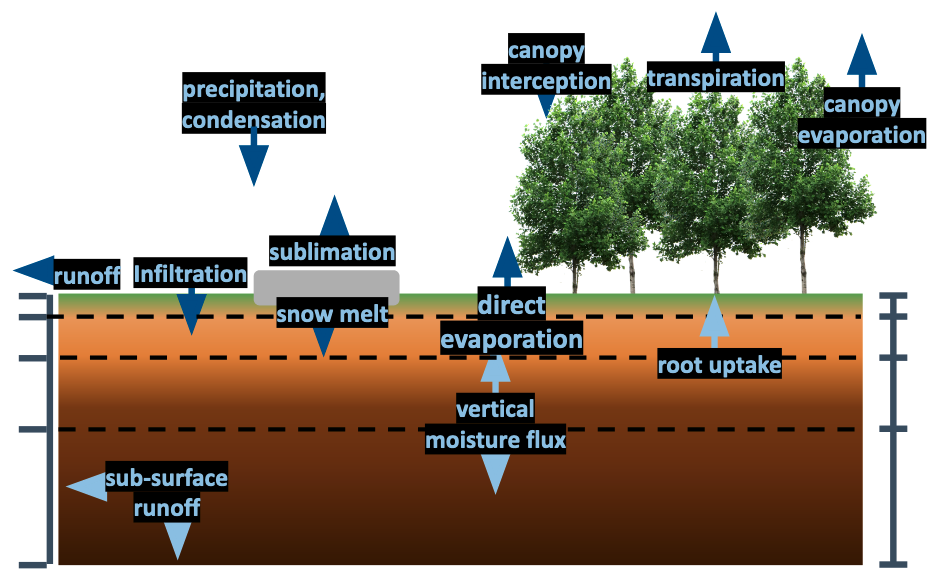
\includegraphics[width=.66\linewidth]{figures/schematic_noah-overview.png}

    \caption{Schematic diagram of the feedbacks contributing to the evolution of soil moisture in Noah-LSM}
    \label{noah-schematic}
\end{figure}

The theoretical framework underpinning Noah-LSM was initially formulated in the 1980s as part of the OSU model, which characterizes boundary layer moisture and energy fluxes as a 2-layer soil model subject to atmospheric forcings. The model expresses the infiltration and movement of water between the soil layers with the diffusive form of the Richards equation \citep{mahrt_two-layer_1984}, direct evaporation using an analytic approximation of the Penman-Montieth relation in terms of atmospheric stability \citep{mahrt_influence_1984}, and basic plant transpiration in terms of vegetation density and soil water content \citep{pan_interaction_1987}. These features form an interdependent system of differential equations that are numerically integrated using a combination of the Crank-Nicholson method and finite-differencing \citep{chen_impact_1997}, which introduces the need for short time steps of 15 or 30 minutes in order for the system to remain numerically stable \citep{cartwright_dynamics_1992}\citep{mahrt_two-layer_1984}.

The OSU model was later significantly improved, renamed to the first generation of Noah-LSM, and coupled with the NCEP Eta forecast model. Noah-LSM expanded the domain to four soil layers of increasing thicknesses (10cm, 30cm, 60cm, and 100cm), improved runoff dynamics by implementing Philip's equation for infiltration capacity \citep{schaake_simple_1996}, and represented the influence of soil texture on moisture transport by introducing bounds on bare-soil potential evaporation that are determined by the soil composition \citep{betts_assessment_1997} \citep{mahfouf_comparative_1991}. The model also features a significantly enhanced representation of vegetation including a more thorough treatment of canopy resistance via a ``Jarvis-type'' model of leaf stomatal control \citep{jarvis_interpretation_1976} \citep{jacquemin_sensitivity_1990}, which accounts for the dependence of transpiration on insolation, air temperature and dewpoint, soil moisture content, and vegetation density. The vegetation effects are scaled by a monthly climatology of normalized difference vegetation index (NDVI) values observed by the NOAA-AVHRR satellite radiometer, which serve as a proxy for green vegetation fraction (GVF) \citep{gutman_derivation_1998} \citep{chen_modeling_1996}, and the depth of root water uptake associated with plant transpiration is determined by a pixel's vegetation class as specified by the Simple Biosphere Model \citep{dorman_global_1989}. Finally, the model's utility was greatly expanded with the addition of a frozen soil and snow pack parameterization incorporating the thermal and hydraulic properties of fractionally-frozen soil layers, the effects of state changes \citep{koren_parameterization_1999}, radiative feedbacks from partial snowpack coverage, and a snow density scheme \citep{ek_implementation_2003}.

Soon after the turn of the millennium, the first generation of NLDAS was under development as part of a multi-institution collaborative effort sponsored by the Global Energy and Water Cycle Experiment (GEWEX) Continental-scale International Projects (GCIP) team. The goal of the project was to incorporate long-term observations of land surface temperature, snow pack depth, and meteorological forcings from multiple sources (in-situ, satellite, radar) into a common framework used to independently evaluate land surface states and energy fluxes with four land surface models including Noah-LSM \citep{mitchell_multi-institution_2004}. Over a domain including the full conterminous United States (CONUS) at $0.125^\circ$ resolution, the models were allowed to spin up over the course of a year, and soil states were recurrently used to initialize subsequent time steps rather than being ``nudged'' to correct for drift. Land cover and soil texture classification over the domain was derived by coarsening the University of Maryland and STATSGO datasets, respectively, from their native 1km resolutions \citep{hansen_global_2000}, surface geometry and elevation is provided by the GTOPO30 dataset \citep{earth_resources_observation_and_science_centeru_s_geological_surveyu_s_department_of_the_interior_usgs_1997}, and the parameter values for soil hydraulic properties were adapted from observations taken at the University of Virginia \citep{cosby_statistical_1984}.

\begin{table}
    \centering
    \begin{tabular}{ l l l l l}
        Forcing & Unit & Source & $\Delta$t & $\Delta$x \\
        \hline
        \multirow{2}{*}{Precipitation} & \multirow{2}{*}{kg m$^{-2}$} & CPC Gauge observations & 24h & 14km \\[-12pt]
        & & WSR-88D retrievals & 1h & 4km \\
        Temperature & K & NCEP NARR & 3h & 32km \\
        Specific Humidity & kg kg$^{-1}$ & NCEP NARR & 3h & 32km \\
        Surface Pressure & Pa & NCEP NARR & 3h & 32km \\
        Wind Velocity & m s$^{-1}$ & NCEP NARR & 3h & 32km \\
        Incident LW Flux & W m$^{-2}$ & NCEP NARR & 3h & 32km \\
        Incident SW Flux & W m$^{-2}$ & GOES, NARR & 3h, 1h & 14km \\
        Green Veg Fraction& \% & AVHRR NDVI & Monthly & 16km \\
        Leaf Area Index & m$^2$ m$^{-2}$ & UMD, AVHRR NDVI& Monthly & 16km \\
        Snow Water Equivalent & kg m$^{-2}$ & Noah-LSM & 14km \\
    \end{tabular}
    \caption{Atmospheric forcings and other time-varying parameters provided by NLDAS-2 at a 1-hourly resolution on the $0.125^\circ$ CONUS grid. Data are resampled using spatial bilinear interpolation, then temporal disaggregation according to \citep{cosgrove_real-time_2003}. NLDAS forcing files also include values for convective available potential energy, the ratio of precipitation from convection, and surface potential evaporation (calculated as in \citep{mahrt_influence_1984}), but these three values aren't currently used as inputs to the models. Snow water equivalent estimates are an output of Noah-LSM by default, but are included as a predictor here under the assumption that they can be provided from a separate model or data assimilation source.}
    \label{forcing}
\end{table}

Attention remained on Noah-LSM in the following years as it continued to support NLDAS and other data assimilation and forecasting systems, which led to a series of improvements introduced alongside the next phase of the NLDAS project. A seasonal effect was added to vegetation by scaling the leaf area index (LAI) by the GVF within bounds determined by the plant type, and transpiration was scaled by a root uptake efficiency factor determined by the proximity of soil temperature to an optimum growth temperature (298 K). Several parameters were adjusted including the influence of vapor pressure deficit on transpiration rate, the minimum stomatal resistance for several plant species, and hydraulic parameters for some soil textures. The aerodynamic conductance coefficient -- an important factor in the strength of moisture and energy fluxes from the surface -- was increased during daylight hours, and a basic anisotropy model was introduced by modifying the albedo of some surfaces in terms of the solar zenith angle \citep{wei_improvement_2011}. Snowpack physics were also modified to improve surface exchange coefficients, and to gradually diminish the snow albedo over the time since the last snowfall \citep{livneh_noah_2009} \citep{liang_simple_1994}. These changes introduce new feedbacks and involve sensitive parameters like LAI which have a strong influence on the model's dynamics \citep{rosero_quantifying_2010}. The retrospective NLDAS-2 data record generated after applying these modifications extends back to 1979, and continues to be updated in a near real-time capacity \citep{xia_continental-scale_2012}.

The NLDAS-2 time-varying retrospective forcings listed in Table \ref{forcing} will serve as the predictors used by the neural networks to forecast the Noah land surface model soil moisture states. Temperature, humidity, pressure, wind speed and heading, and longwave flux are derived exclusively from the National Centers for Environmental Prediction (NCEP) North American Regional Reanalysis (NARR) data product. As part of the downscaling procedure from their native 32km resolution to the 1/8$^\circ$ NLDAS domain, a lapse rate adjustement is applied to the temperature and humidity fields based on the elevation profile. Downward shortwave radiative flux is calculated using a blend of NARR and hourly Geostationary Operational Environmental Satellite (GOES) data, with a ratio-based bias correction based on \citep{berg_impact_2003} applied to account for a known positive bias in NARR-reported downward shortwave flux, and to mitigate discontinuities arising from the merger the two data sources \citep{pinker_surface_2003} \citep{xia_continental-scale_2012-1}. Precipitation receives a special treatment in order to ensure sufficient spatial resolution and consistency; the Climate Prediction Center (CPC) daily gauge-based product \citep{chen_assessing_2008} serves as the baseline, which is temporally disaggregated to 1 hour resolution using National Weather Service WSR-88D radar retrievals \citep{fulton_wsr-88d_1998}. In regions lacking radar coverage, the disaggregation is completed using a weighted combination of the CPC's satellite-derived estimates from morphed passive-microwave and infrared observations (CMORPH) \citep{joyce_cmorph_2004}, and the CPC Hourly Precipitation Dataset (HPD), with NARR data as a final fallback \citep{baldwin_ncep_1997}.  Although both the LAI and GVF vegetation parameters are based on multi-year monthly averages, they are disaggregated to an hourly resolution in order to be smoothly variable \citep{wei_improvement_2011}, and are thus treated like an atmospheric forcing in this work.

\section{Calibration and Validation of Noah-LSM}

During the development of Noah-LSM, researchers integrated information from a variety of observational datasets in order to calibrate and validate the soil moisture, energy flux, and radiative components of the model outputs. The initial field campaign data that bootstrapped development of the OSU model precursor came from the First International Satellite Land Surface Climatology Project Field Experiment (ISLSCP FIFE) \citep{sellers_overview_1992}, which utilized averaged evaporation data data from 10 stations in a 15x15km grassland area during the warm season of 1987. The OSU model showed strong performance in capturing the seasonal and diurnal cycle of evaporation, soil moisture, heat fluxes, and skin temperature, however struggled during wet periods due to an over-estimation of evaporation caused by the canopy resistance formulation \citep{chen_modeling_1996}.

Based on these results, others utilized further observations to integrate and parameterize new processes within Noah-LSM in order to mitigate the shortcomings. For example, and the bare surface evaporation and vegetation schemes were improved by \citep{betts_assessment_1997} based on four 48-hour intensive observation periods within FIFE, surface runoff parameters were improved by \citep{schaake_simple_1996} based on long-term USGS stream discharge datasets from gauged basins in Oklahoma, Mississippi, and North Carolina. The radiation balance and heat flux magnitudes from Noah-LSM were evaluated with respect to a full year of data from 7 sites in the Oklahoma Mesonet by \citep{sridhar_validation_2002}, who found a slight positive bias in flux magnitudes, but overall good performance with root mean squared error rates for all fluxes falling below 2.5 $MJ\,m^{-2}\,d^{-1}$. Fluxes, temperatures, radiation, and soil moisture were further validated by \citep{robock_evaluation_2003} with respect to Oklahoma Mesonet and ARM/CART surface station observations from 1998 and 1999; they found that Noah-LSM performed better than all other models in the NLDAS framework, but had a positive bias in soil moisture around 7\%, which was postulated to be the consequence of inadequacy in the static soil parameterization.

Snow and frozen soil posed a particular issue during the early development of Noah-LSM, as neglecting the physics of partially-frozen soil, fractional snow cover, and variable snow density resulted in significant underestimates in soil moisture, and high error rates in soil temperature. These shortcomings were addressed by the new physics introduced by \citep{koren_parameterization_1999}, which were calibrated based on soil moisture, temperature, and snow water equivalent observations from Rosemont, Minnesota during the 1995-1996 cold season. The ~20\% under-estimation of lower-layer soil moisture and high error in soil temperature were greatly diminished as a consequence of the changes. Significant snowpack volume under-estimates were also addressed by \citep{livneh_noah_2009} using SNOTEL station snow water equivalent data, and subsequently by \citep{barlage_noah_2010} based on problems noted by \citep{pan_snow_2003} using both SNOTEL and SNODAS data. In combination, these process improvements reduced the low bias to about 15\%, and improved the snow water equivalent correlation with the observations to about 80\%.

In the lead-up to the second generation of NLDAS, \citep{wei_improvement_2011} implemented further improvements to warm-season processes which were validated based on ARM/CART surface flux stations as well as GOES satellite retrivals of land surface temperature during the 1998 and 1999 warm seasons. The consequence was a reduction in spring-season positive bias in latent from 80 $W\,m^{-2}$ to about 20 $W\,m^{-2}$ and land surface temperature with a correlation of about .85, a slight negative bias of $-1.26\,K$, and root mean squared error around $3.08\,K$. Additionally, \citep{xia_evaluation_2014} validated NLDAS-2 modeled soil moisture against 20 years of monthly data from the Illinois climate network (1986-2004), 6 years of daily data over 72 sites from the Oklahoma Mesonet (1997-2002), and 8 years of daily data from 121 SCAN sites (2002-2009). They found that Noah exhibited a mean monthly anomaly correlation of .82 in the first 2m, which was stronger in the warms seeason but struggled when the ground was frozen or snow was present, especially in lower two soil layers. The daily mean anomaly correlation from the Oklahoma Mesonet data was greater than .8 in the lower layers and .77 in the surface layer, while the monthly averages were all above .85 with about 15\% relative MAE and a relative bias around -15% for all three tested layers. Regional analyses with respect to the widely-dispersed SCAN stations indicate substantial variability in performance; Noah-LSM struggled with the surface layers in the Northeast US with a correlation of only about .2, but was consistently better than .5 correlation elsewhere, especially in the Great Plains and Northwest. The midwest also exhibited a large dry bias, which is likely the consequence of a lack of irrigation information in the cropland-dominated region.

Finally, an entropy-based decomposition of uncertainty was employed by \citep{nearing_benchmarking_2016} to quantify the components of error in Noah-LSM caused by improper characterization of forcings, model dynamical structures, and model parameters. By comparing to soil moisture observations from 49 SCAN sites and 50 AmeriFlux stations active between 2001 and 2011, they determined that inadequate model parameters like soil texture and vegetation classification were the greatest sources of uncertainty in the soil moisture profile, while biased input forcings were the dominant cause of uncertainty for energy fluxes.

\section{Distinctions in Modeling Techniques}

\begin{figure}[h]
    \centering

    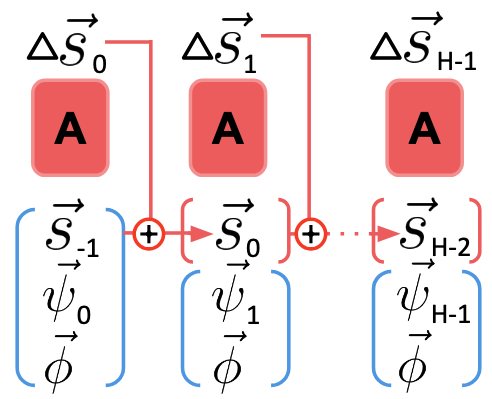
\includegraphics[width=.66\linewidth]{figures/schematic_scann.png}

    \caption{Diagram of a self-cycling discrete-time dynamical system with no hidden state. At each time, nonlinear operator \textbf{A} maps an initial state $\vec{s}_{k-1}$, exogenous forcing $\vec{\psi}_k$, and time-invariant parameters $\vec{\phi}$ to a new state $\Delta \vec{s}_k$, used to initialize the subsequent time step, and so forth until $H$ predictions have been made.}
    \label{scann}
\end{figure}

\subsection{Noah-LSM as a Discrete Dynamical System}

At its core, Noah-LSM is a collection of coupled differential equations that express the total derivative of land surface states $\frac{d\vec{s}}{dt}$ in terms of the current state $\vec{s}$, forcing $\vec{\psi}$, and time-invariant properties of each grid cell $\vec{\phi}$. Since the model is implemented as an algorithmic procedure and is not continuously differentiable, we will use the notation $\frac{\Delta \vec{s}_k}{\Delta t} \approx \mathbf{A}(\vec{s}_{k-1}, \vec{\psi}_k, \vec{\phi}, \Delta t)$ to refer to the model as a transition function evaluated at a discrete time step $\Delta t$, such that the system evolves as a dynamical system described by Equation \ref{dynamical}.

\begin{equation}\label{dynamical}
    \vec{s}_k = \vec{s}_{k-1} + \mathbf{A}(\vec{s}_{k-1}, \vec{\psi}_k, \vec{\phi}_k, \Delta t) \cdot \Delta t
\end{equation}

Here, $\vec{s}_k$ refers to the model's dynamic state variables like snow pack depth, soil moisture and temperature, and canopy storage, $\vec{\psi}_k$ encodes the covariate atmospheric variables from Table \ref{forcing} (which are derived from weather forecasts or observations), and $\vec{\phi}$ includes time-invariant coefficients of the governing equations like vegetation type/fraction, soil texture, and slope/elevation. As a matter of convention, the time step $k=0$ refers to the first perturbation of the initial state after applying the model's first increment change estimate, and includes the forcings that informed that perturbation, consistent with the relationships depicted by Figure \ref{scann}.

To generate a time series, Noah-LSM numerically integrates the system of equations using Euler and Crank-Nicholson techniques, which explicitly evaluate the differential equations at several time intervals per computational time step in order to estimate the nonlinear change in state, which evolves continuously in the real system being modeled. It is crucial that the increment change in time remains small between evaluations of the model (15min for NLDAS-Noah) to mitigate truncation error from the assumption of local linearity \citep{mitchell_multi-institution_2004} \citep{cartwright_dynamics_1992}. As Figure \ref{scann} suggests, the model does not retain any ``hidden'' internal information that is updated between timesteps; at each point, the information available to determine the new change in state is limited to the input domain of the model.

\subsection{Process-based vs Data-driven Models}

The process-based approach of numerical models like Noah-LSM is practically and epistemologically distinct from data-driven techniques like deep learning. In a process-based paradigm, the inductive biases that govern the model's behaviors can be explicitly understood since they are based on a characterization of the physical system which is derived from theoretical knowledge. Some uncertainty is introduced by the input data, and is shared among all model types; this includes uncertainty from noise and interpolation of forcing observations, discrete treatment of surface types, etc. Aside from that, model error in process-based models arises from sources including inadequacy of the theory for describing the system (that is, phenomena which are neglected or misrepresented, and become a source of unexplained variance), and truncation error accumulated from the approximation techniques used to solve the model's governing equations. Explicit understanding of the reasons for the model's behavior has the advantage of being interpretable, in the sense that particular systems within the model can be independently evaluated and blamed for contributing uncertainty. Additionally, granting the ability to impose absolute constraints within the model structure ensures the outputs fully adhere to some physical requirements, such as conservation of water and energy. Nonetheless, the onus falls entirely on the model developer to adjust many details of the implementation of the processes. The act of tuning a numerical model's parameters often implies postulating a source of uncertainty, addressing it by manually manipulating coefficients or introducing new systems within the governing equations, and then evaluating the impact of the changes using correlational analysis with a subset of the available data. This can be a laborious process, and typically results in the gradual accumulation of feedbacks and complexity within the model.

In contrast, many data-driven approaches to modeling physical systems -- deep learning in particular -- sacrifice the explainability and rigorous physicality of their estimates in exchange for developing a statistically optimal approximation of the relationship between the input and output domains by any means available. Although the overall algorithmic structure of the ANN is established by the developer -- typically based on broad heuristics from past literature and experimentation -- very little control can be asserted over the particular means by which predictions are determined from inputs. Instead, the effectiveness of the ANN's performance is characterized in terms of a differentiable loss function (also known as the objective or cost function) which may be defined by the developer, and which is fundamentally (though indirectly) important for determining the solution developed in the training phase.

An ANN's learnable parameters refer to the real-valued elements of a series of arbitrarily-sized square matrices encoding affine transformations. Each ``layer'' of the ANN is comprised of one of these affine transformations followed by an element-wise nonlinear operation on its output, and the full ANN typically consists of multiple layers which are combined via composition or any kind of differentiable arithmetic operation. During training, all of the ANN's learnable parameters are iteratively adjusted by estimating the gradient of the loss function with respect to the parameters (given batched subsets of the predictor/target data pairs) then determining the direction and magnitude by which the parameters in each of the layers should be modified with an algorithm called backpropagation \citep{rumelhart_learning_1986}. The general strategy of determining the sensitivity of the loss landscape to changes in the ANN's parameters, and tweaking them accordingly, is referred to as gradient descent. Given at least 2 layers (which constitutes the definition of a \textit{deep} ANN), the network is theoretically capable of expressing an arbitrary decision boundary or multivariate function given a sufficient number of parameters \citep{hornik_multilayer_1989}. This high level of expressivity enables the network to learn complex relationships and generalizations among high-dimensional parameters, given repeated exposure to instances of these relationships during training.

The principle of ANNs using high-dimensional nonlinear correlations rather than explicit processes to model the correspondence between two datasets is powerful because they can approximate a highly nonlinear regression without numerically integrating a complex algorithm, and they can learn their parameterization based on a large volume of data without manual intervention. The quintessential drawback of relying on a black-box approach, though, is that models may perform poorly for no apparent reason, or may perform well for a fraught reason. For example, in one commonly-invoked anecdote described by \citep{lapuschkin_unmasking_2019}, an image classifier over-performing but failing to generalize at identifying horses in a grassy field was found to actually rely on the presence of the watermark of a particular equestrian photographer whose work was a part of the training data. As such, only regarding bulk statistics and loss performance as indicative of a model's success is insufficient to consider it trustworthy. In a data-driven paradigm, then, the role of the ANN developer is to facilitate effective and reliable learning through careful training data curation, congnizant loss function and model architecture design, and thorough evaluation of the model's behavior in local and global scenarios throughout the input domain in order to ensure the effectiveness and consistency of predictions in a variety of inference settings.

Furthermore, it is important to note that in the current scope of this work, it is not possible for the ANNs to leverage their expressivity to out-perform the numerical model. Since the ANNs presented here are merely emulating the processes that are programmed into Noah-LSM, it isn't reasonable to expect the models to form a more accurate representation of real soil dynamics. Nonetheless, it is conceivable that future work could utilize a similar approach to \citep{o_global_2021} in order to integrate observational data into the training domain alongside model data, or to use it as a prediction target. The merger of these two data sources could aid in improving a data-driven model beyond the limitations of a numerical model's structure.

\section{Deep Learning of Time Series}

\begin{figure}[h!]
    \centering

    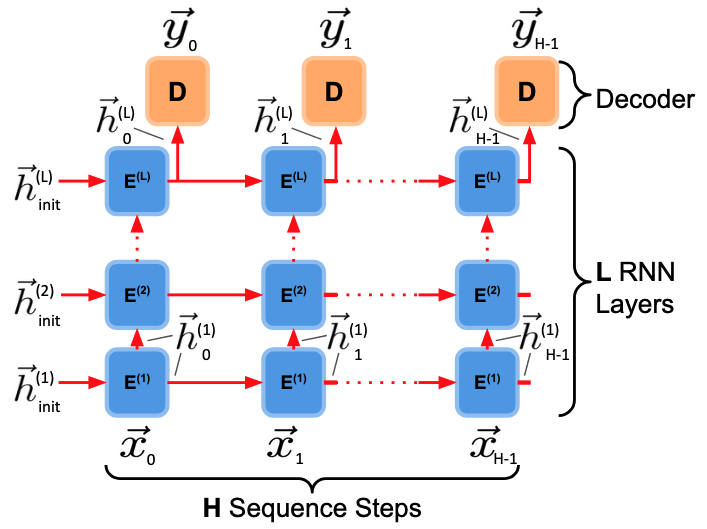
\includegraphics[width=.95\linewidth]{figures/schematic_abstract-rnn.png}

    \caption{Schematic representation of an abstract sequence-to-sequence RNN with multiple layers.}
    \label{schematic-rnn}
\end{figure}

The most simple variant of an ANN is referred to as a feed-forward neural network (FNN), which consists of a series of composed layers (see previous section) mapping the input vector directly to the output. Although a FNN is theoretically capable of simulating Noah-LSM in the manner of Figure \ref{scann}, inductive biases are commonly introduced in model architectures in order to promote efficiency, explainability, stability, and parsimony. For example, most neural networks used for sequence modeling like the recurrent neural networks (RNNs) in Figure \ref{schematic-rnn} maintain one or more ``hidden'' latent parameters $\vec{h}$ with an arbitrary number of dimensions. This vector is modified and passed along by each subsequent iteration, giving the network the ability to make temporal generalizations and propagate information to future predictions. Although $\vec{h}$ is typically difficult to interpret directly, the gradient descent process incentivizes the network to preserve and consolidate information that is needed to accurately generate the full sequence of predictions. This construct is promising for improving the models' ability to estimate soil dynamics because characteristic drydown curves are known to exhibit hysteresis depending on their recent patterns of wetting and drying \citep{haines_studies_1930}. %Each of the following network architectures ultimately aim to improve the information quality of the latent vector by implementing algebraic structure, introducing statistical uncertainty, and encouraging sparsity.

\begin{equation}\label{eq_rnn}
    \begin{split}
        %\vec{h}_k^{(1)} &= \mathbf{E^{(1)}}\left(\vec{h}_{k-1}^{(1)},\, \vec{\psi}_k,\, \vec{\phi}\right) \\
        \vec{h}_k^{(1)} &= \mathbf{E^{(1)}}\left(\vec{h}_{k-1}^{(1)},\, \vec{x}_k\right) \\
        \vec{h}_k^{(j)} &= \mathbf{E^{(j)}}\left(\vec{h}_{k-1}^{(j)},\, \vec{h}_k^{(j-1)}\right) \\
        \vec{y}_k &= \mathbf{D}\left(h_k^{(L)}\right)
        %\vec{s}_{k+1} &= \vec{s}_{k} + \mathbf{D}\left(h_k^{(L)}\right)
    \end{split}
\end{equation}

The RNNs discussed here will follow the general structure described by Equation \ref{eq_rnn}, which is consistent with the abstract architecture diagrammed in Figure \ref{schematic-rnn}, and follows the typical approach for constructing RNNs as outlined in \citep{russell_artificial_2020}. The architecture consists of L encoder layers (\textbf{E}$^{(1)}$-\textbf{E}$^{(L)}$) which generate H top-layer latent vectors corresponding to each of the prediction times, and 1 layer of decoder weights \textbf{D} which converts each of the top-layer latent vectors to a prediction for the increment change in state $\Delta \vec{s}$ between the current timestep and the next one. Parameters for \textbf{E} and \textbf{D} are shared across timesteps, however each of the L layers have distinct parameters. Here, $\vec{h}_k^{(1)}$ is a member of the time series of first-layer latent vectors given the arguments $\vec{x}_k$ and the latent vector from the previous first-layer timestep $\vec{h}_{k-1}^{(1)}$. Moving upward, $\vec{h}_k^{(j)}$ is an intermediate-layer latent vector such that $j \in [2,\,L]$, and when $k=0$ (the first horizon timestep), $\vec{h}^{(s)}_{-1} = \vec{h}^{(s)}_{\text{init}}$ for any layer $s$. In many cases, the initial hidden states $\vec{h}^{(s)}_{init}$ are randomized or set to zero, however in this project we use a separate spin-up RNN to establish them, as will be discussed in the Methodology section.

\begin{figure}[h!]
    \centering

    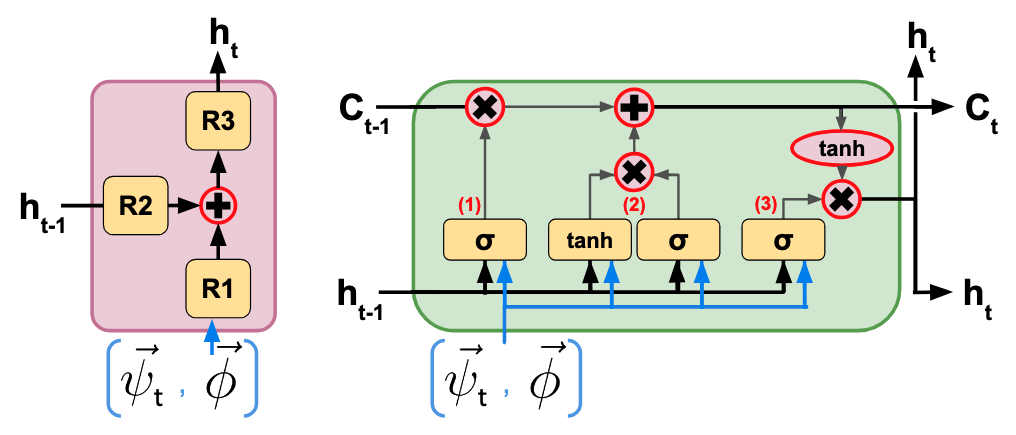
\includegraphics[width=.95\linewidth]{figures/schematic_rnns-both.png}

    \caption{Schematic representation of individual RNN cells, the na\"ive RNN (left), and the LSTM (right)}
    \label{rnns-both}
\end{figure}

The term RNN does not refer to a specific neural network architecture, but rather the category of architectures that share their weights across sequence steps. The sub-network unit of weights applied at each timestep (\textbf{G} or \textbf{E} in Figure \ref{s2s-default}) is referred to as a RNN cell, and must contain internal structure for converting inputs from lower layers and the previous timestep into an output. Unlike traditional ANNs which use backpropagation to train on single input-output pairs, each cell must balance the penalty of its loss gradient between contributions from the input at each timestep with contributions from the latent vector of the previous timestep. To accommodate this difference, RNNs are trained using a special type of gradient descent called backpropagation through time, which balances the loss with respect to the two input sources, and accumulates it across all timesteps before updating each cell's parameters.

The most basic form of the RNN architecture (diagrammed on the left side of Figure \ref{rnns-both}) consists of 3 separate affine operations. As shown in the figure, R1 and R2 convert the lower-layer and previous-timestep vectors, respectively, into two uniformly-sized internal latent vectors. The sum of these internal vectors are transformed by a third affine operation, R3, into the cell's output, which is passed along to the higher layer and subsequent steps within the same layer.

This style of na\"ive RNN is vulnerable to the so-called vanishing or exploding gradient problem, which arises from the fact that the cell output is the direct product of learned matrix operations. Since during training each cell's weights are updated recurrently based on many sequence steps, the loss gradient with respect to each learned parameter can become incredibly sensitive to changes in each parameter. This can cause weights to become very close to zero, or to diverge to very large numbers, which halts the learning process \citep{mozer_focused_1995}. Furthermore, since the latent state passed between sequence steps undergoes a nonlinear transformation at each instance of the cell, it is more tenuous for the network to sustain information over a long context of past observations.

The LSTM architecture addresses these shortcomings by maintaining a separate hidden state $\vec{C}_t$ called the context vector. Rather than being generated by a matrix operation at each step, the context vector is only modified from the previous step's value using the output of a series of three ``gates.'' These gates (numbered in Figure \ref{rnns-both})  include (1) the ``forget gate'', which uses a FNN to select a vector of values in the range (0,1). The forget vector is multiplied element-wise by $\vec{C}_{t-1}$ in order to selectively emphasize or diminish its activation. The ``update gate'' (2) transforms the inputs into a new coefficient vector in the range (-1,1), which is added to the context vector in order to retain information from the current time step. Finally, the ``output gate'' (3) generates a vector of multiplicative coefficients in the range (0,1) used to scale the new context vector $\vec{C}_t$ to the output latent state $\vec{h}_t$ \citep{hochreiter_long_1997}. The context vector remains stable compared to a hidden vector that is recurrently operated on by the same weight matrix, which facilitates the network to learn over a longer sequence interval.

The Transformer architecture has dominated many sequence modeling tasks in recent literature thanks to the key innovation of multi-head self-attention (MSA), which enables the architecture to learn complicated relationships between individual members of the input sequence regardless of their relative position. Additionally, transformers are efficient to train in parallel, unlike RNN architectures which rely on a chain of sequential operations, which makes them straightforward to train on a massive scale \citep{vaswani_attention_2017}. The results for natural language processing (NLP) \citep{devlin_bert_2019} and image classification \citep{dosovitskiy_image_2021} tasks are impressive, however there are several key drawbacks that make them less appealing for a time series generation task like this one.

First, the memory cost of a transformer scales quadratically with sequence length since MSA learns parameters relating every possible combination of input steps. This is compounded with the fact that the full input sequence needs to be re-initialized with every step during inference. These properties are a direct trade-off with the Transformer's ability to train separate sequence steps in parallel. Furthermore, unlike RNNs and CNNs, Transformers don't have an inherent notion of order. In problems like NLP where sequence position conveys some information, a simple form of locality is introduced by adding a positional embedding vector directly to the inputs. Prior literature shows that transformers equipped with positional embedding still perform no better on basic time series forecasting tasks than a simple 2-layer FNN \citep{zeng_are_2022}. For these reasons, although MSA is a very powerful tool for many applications, we will be neglecting this very popular architecture in this work.

\chapter{Chapter 3. Data and Methodology}

\section{Dataset Overview}

This section includes a description of the storage of and framework used to interface with the data, insights on the value distributions and spatial variability of the input forcings from NLDAS-2, as well as a look at similar bulk properties of the target soil moisture states and governing processes within Noah-LSM. In this work, we define our valid domain to include all points falling within the conterminous United States, excluding those points within the NLDAS-2 domain falling with Canada and Mexico. We also exclude points that are classified as ``water,'' ``bedrock,'' or ``other'' in the STATSGO dataset, since they do not correspond to meaningful hydraulic properties, and have idle time series. What remains are 50,875 candidate grid cells within a 224x464 pixel domain.

\subsection{Data Storage System}

The data used in this project were acquired from the Goddard Earth Sciences Data and Information Services Center's Distributed Active Archive Center (GES DISC DAAC) in May of 2024. The DAAC archives the NLDAS-2 forcings and corresponding Noah-LSM model outputs as separate hourly files in a GRIB1 format, of which we downloaded the full 12-year time series from January 1, 2012 to December 31, 2023. This subset constitutes 210,384 files with a total size of just over 891.38 GB.

Since this project concerns developing 2-week time series of the forcings on a per-pixel basis, it would be inefficient to extract data from several hundred files for each sequence sample. Furthermore, it is widely recognized in deep learning that input/target pairs from heterogeneous datasets should be globally shuffled during the training process, as outlined by \parencite{nguyen_why_2022}. This is because local subsets may have distribution characteristics that are distinct from the full dataset, so as the model trains on an unshuffled dataset, the loss gradients it experiences may encourage it to converge on a locally-optimal solution that does not generalize well to the overall task. Shuffling is especially salient for geoscience datasets like this one, which are highly spatially and temporally heterogeneous. With this in mind, the overhead from file I/O operations would be prohibitive for sporadically drawing samples from throughout the GRIB dataset during training or inference.

To address this problem while maintaining the spatiotemporal structure of the data, we develop a custom file standard using the HDF5 format -- hereafter referred to as the \texttt{timegrid} -- and extract the full 12-year NLDAS and Noah-LSM record as a collection of them. The HDF5 format offers a system for memory-mapped data chunking in multiple dimensions, which means the data therein can be sparsely buffered and accessed on a per-chunk basis without loading the entire file into memory: a considerable advantage for thoroughly shuffling or accessing subsets of contiguous data within large files. In practice, each timegrid contains 3 years of data covering 1/6 of the spatial domain, and stores the 4-dimensional time-varying data (time, latitude, longitude, data type), 3-dimensional static data (latitude, longitude, data type), and timestamps alongside a string-serialized attribute dictionary. The attributes contain information on abbreviated and full data type names, ordering, units, and sources, which are sufficient to inform a variety of accessor methods with a wealth of downstream use cases.

\subsection{Regional Variance of Input Data}

\begin{figure}[h!]
    \centering
    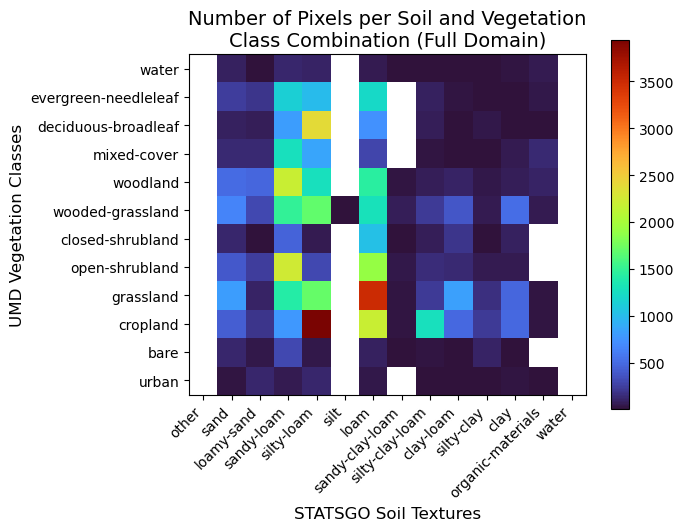
\includegraphics[width=.75\linewidth,draft=false]{figures/static_soil-veg-combos.png}
    \caption{Full-domain combination matrix of vegetation and soil classes.}
    \label{static-combos}
\end{figure}

\begin{figure}[hp!]
    \centering
    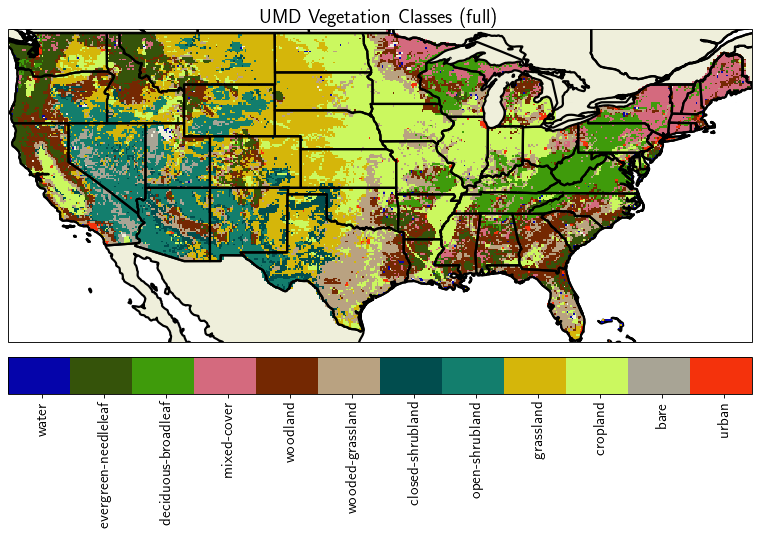
\includegraphics[width=.85\linewidth,draft=false]{figures/static_umd-veg-classes_full.png}
    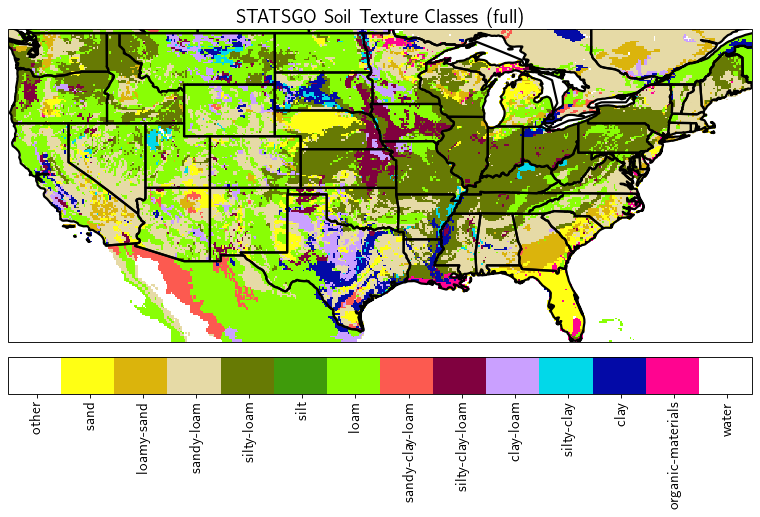
\includegraphics[width=.85\linewidth,draft=false]{figures/static_statsgo-soil-classes_full.png}
    \caption{Spatial distribution of vegetation and soil classes.}
    \label{static-classes}
\end{figure}

\begin{figure}[hp!]
    \centering
    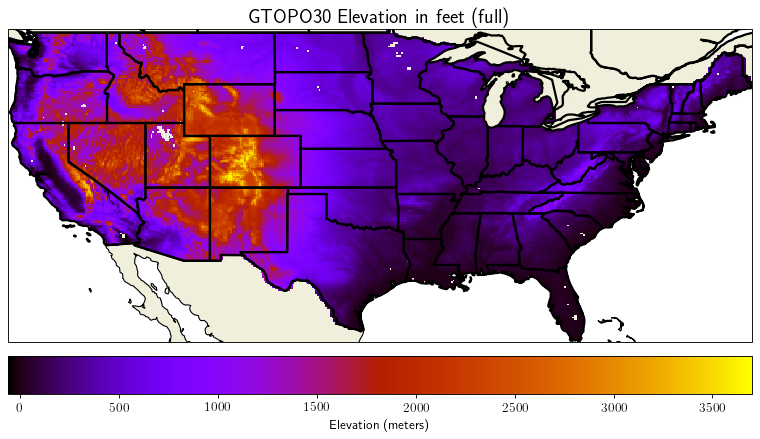
\includegraphics[width=.85\linewidth,draft=false]{figures/static_elev_full.png}
    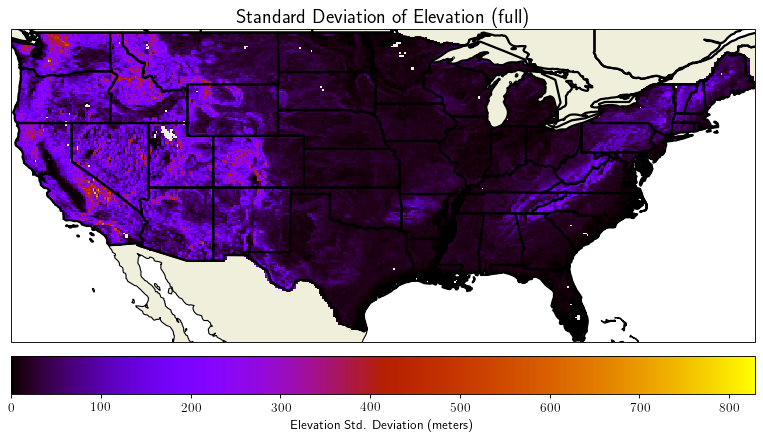
\includegraphics[width=.85\linewidth,draft=false]{figures/static_elev-stdev_full.png}
    \caption{Elevation and standard deviation of elevation on the CONUS domain.}
    \label{static-elevation}
\end{figure}

One important aspect of the NLDAS-2/Noah-LSM datasets is the relationship between static and dynamic parameters, and the regional variance of both of these input types. Given any particular forcing time series, the subsequent land surface response is modulated by values for vegetation type, soil texture, slope, slope aspect, and a drainage parameter referred to as slope type, which are consistent per-pixel throughout the dataset. In this work, we will only train models informed by the first four. Slope and aspect were left out because within Noah-LSM they are only used within the snowpack parameterization \parencite{barlage_noah_2010}, and snow is generally not a target variables for the models presented here. Furthermore, slope correlates strongly with the standard deviation of elevation. Slope type is not well-documented in the model, and was not considered during training, but had a noticable effect on some of the results. In retrospect, these inputs may have increased the information available to the models for estimating the transference of water from snow melt to the soil layers, especially in mountainous regions like the Rocky Mountain and Sierra Nevada ranges. An evaluation of the impact of these parameters on model results is left for future work. Elevation parameters are not directly utilized within Noah-LSM, but it is used to perform orographic regressions on pressure, temperature, humidity, and precipitation while resampling forcing data. Thus it is included as a training input because it could be useful as a predictor that indicates processes relevant to mountain snowpack dynamics.

As described in the background, the vegetation classes encode the properties of the canopy relevant to precipitation interception and land surface shading, the efficiency of plant transpiration at removing water from the soil, and the number of layers from which water is drawn (that is, the rooting depth). Since the vegetation parameter is discretely categorical within the Noah-LSM algorithm, we employ a special method of introducing them into the model called class embedding, which is elaborated upon in the next subsection.

\begin{table}[H]
    \centering
    \scriptsize
    \caption{Soil hydraulic properties associated with each texture class from \parencite{cosby_statistical_1984}.}
    \begin{tabular}{c|c|c|c|c|c|c }
Texture & \thead{Porosity \\ ($m^3/m^3$)} & \thead{Field Cap. \\ ($m^3/m^3$)} & \thead{Wilting Pt. \\ ($m^3/m^3$)} & \thead{B Param. \\ (dimless)} & \thead{Hydr. Cond. \\ ($mm/s$)}\\
\hline
Sand & 0.395 & 0.275 & 0.023 & 4.050 & 0.968 \\
Loamy Sand & 0.421 & 0.317 & 0.028 & 4.260 & 0.077 \\
Sandy Loam & 0.434 & 0.343 & 0.047 & 4.740 & 0.029 \\
Silty Loam & 0.476 & 0.389 & 0.084 & 5.330 & 0.015 \\
Silt & 0.476 & 0.389 & 0.084 & 5.330 & 0.015 \\
Loam & 0.439 & 0.356 & 0.066 & 5.250 & 0.019 \\
Sandy Clay Loam & 0.404 & 0.337 & 0.069 & 6.770 & 0.024 \\
Silty Clay Loam & 0.464 & 0.406 & 0.120 & 8.720 & 0.011 \\
Clay Loam & 0.465 & 0.403 & 0.103 & 8.170 & 0.013 \\
Silty Clay & 0.468 & 0.420 & 0.126 & 10.390 & 0.007 \\
Clay & 0.457 & 0.416 & 0.135 & 11.550 & 0.005 \\
Organic & 0.464 & 0.377 & 0.069 & 5.250 & 0.019 \\
\end{tabular}
    \label{soil-texture-table}
\end{table}

%The soil texture class corresponds to a variety of hydraulic properties identified by \parencite{cosby_statistical_1984}, which include field capacity, hydraulic conductivity, porosity, wilting point, matric potential, and Skempton's pore water pressure (``B'' parameter). These describe physical characteristics of the soil-water system including the rate of downward percolation of water, the efficiency and limits of plant water uptake, the speed of infiltration, and the total amount of water that soil can contain per unit volume. The basic observable feature of soil that determines all of the hydraulic properties is the size distribution of its constituent particles, which is often articulated as the mass fraction of sand, silt, and clay components within the soil. In the interest of providing the models with real-valued inputs having relatively low dimensionality, these three texture components will serve as the representation of soil texture for the ANNs trained here.

In Noah-LSM, each pixel is assumed to have a vertically uniform soil texture throughout the column. The texture associated with each pixel is based on the surface of the 11-layer spatial soil dataset developed by \parencite{miller_conterminous_1998}, as pictured in Figure \ref{static-classes}. Each texture category is mapped to a variety of hydraulic properties mainly based on measurements taken by \parencite{cosby_statistical_1984}. These parameters include field capacity, hydraulic conductivity, porosity, wilting point, matric potential, and the exponential``B'' parameter of the soil water retention curve. The basic observable feature of soil that determines all of the hydraulic properties in the scheme used by the model is the size distribution of its constituent particles, which is often articulated as the mass fraction of sand, silt, and clay components within the soil. In the interest of providing the models with real-valued inputs having relatively low dimensionality, these three texture components will serve as the representation of soil texture for the ANNs trained here.

Table \ref{soil-texture-table} lists each of the soil textures alongside their hydraulic parameters. We will now briefly discuss how each parameter affects soil dynamics based on \parencite{dingman_physical_2014}. The porosity is the ratio of a volume of soil that is not occupied by solids like minerals and organic compounds, which determines the limit of the material amount of water that the soil can contain at saturation. Counterintuitively, coarse soils like sand have lower porosity than clay-dominant soils because the grain shapes associated with sand are packed more efficiently than clay, and as such sand can have a lower maximum water capacity per unit volume. Ignoring the influence of evapotranspiration, gravity will cause water to gradually drain downward through unsaturated soil at an exponentially decreasing rate consistent with the Richards Equation. Under these circumstances, the field capacity of a soil is the volume fraction of soil water at which the rate of drainage is negligible. As such, when the soil water content is below the field capacity, the only processes that further decrease the water content are evapotranspiration and capillary diffusion to a drier adjacent soil layer. The enhanced adhesive forces associated with finer-grained soils like clay grant them a field capacity that is much closer to their porosity than a coarser soil like sand, so for finer soils evapotranspiration and diffusion will dominate the dynamics except when the soil is close to saturation. The wilting point is defined in terms of volume fraction of soil water based on the suction pressure plants are able to exert on the soil in order to remove water, which is typically assumed to be $-1,470\,kPa$. Once the soil reaches the wilting point, the process of plant transpiration ceases, and the only process that may still diminish water in the soil layer is diffusion.

The hydraulic conductivity of a soil describes the rate at which water can move through the soil against the friction of the soil matrix. Soils with large pore sizes like sand have a dramatically higher hydraulic conductivity than finer soils, and as such can transmit infiltrated water much more rapidly to lower layers. The values given in Table \ref{soil-texture-table} refer to the hydraulic conductivity at saturation, however in practice the hydraulic conductivity has a highly nonlinear relationship with the soil water content such that it decreases following an exponential curve that must be empirically determined. This relationship is defined in terms of the B parameter, which is inversely proportional to the mean pore size of each soil texture. While the hydraulic conductivity of a soil at saturation is a constant, the hydraulic conductivity of fine-grained soils with a large B parameter decreases much faster as the soil dries compared to coarser soils, which maintain relatively large hydraulic conductivities at mid or low-range water content. Soil water diffusion is a separate important term in the Richards equation which governs the movement of water across a moisture gradient between layers as a consequence of capillary action, which enables the upward percolation of water, and moisture exchange between soil layers when the water content is below the field capacity. Diffusion is also defined in terms of an exponential relationship with the B parameter, described a nonlinear differential equation without an analytic solution. Coarser soils tend to have higher diffusivities close to saturation that peak just below saturation, while finer soils have lower diffusivities that more rapidly diminish as the soil dries.

The interplay between plant water uptake and soil water dynamics as governed by the static inputs represents a considerable source of complexity within Noah-LSM. Furthermore, as Figure \ref{static-combos} demonstrates, the distribution of combinations of soil and vegetation categories is extremely non-uniform, which makes it more difficult for ANNs to learn solutions that are general. Figure \ref{static-classes} shows the geographic locations of vegetation and soil classes. The most common class combination is silty-loam soil types juxtaposed with cropland, with 3,945 members found dominantly in the Midwest and lower Mississippi river basin, with some contribution from the Columbia Plateau in Washington and Eastern Nebraska. Next most common are the 3,490 pixels in loamy grasslands, which are distributed widely throughout the West US including the high plains, Western Texas and New Mexico,  Utah, and Idaho. The remaining combinations all have fewer than 2,500 members within the domain. Sand and clay dominated soils form the upper and lower extremes of soil particle size, respectively, and thus have rather different soil water characteristics. The sandiest soils are found in Southern Coastal Plains, Michigan, Texas, the Nebraska Sandhills, and the desert Southwest. Clay soils are relatively rare compared to silty and sandy soils, and considerably more spatially heterogeneous. They are mainly found in tight groupings around Central Texas, the Mississippi Alluvial Plain, Eerie Lake Plains, and the Missouri River Basin in South Dakota. Despite their infrequency, clay soils span the full range of surface classes.

\begin{figure}[h!]
    \centering
    %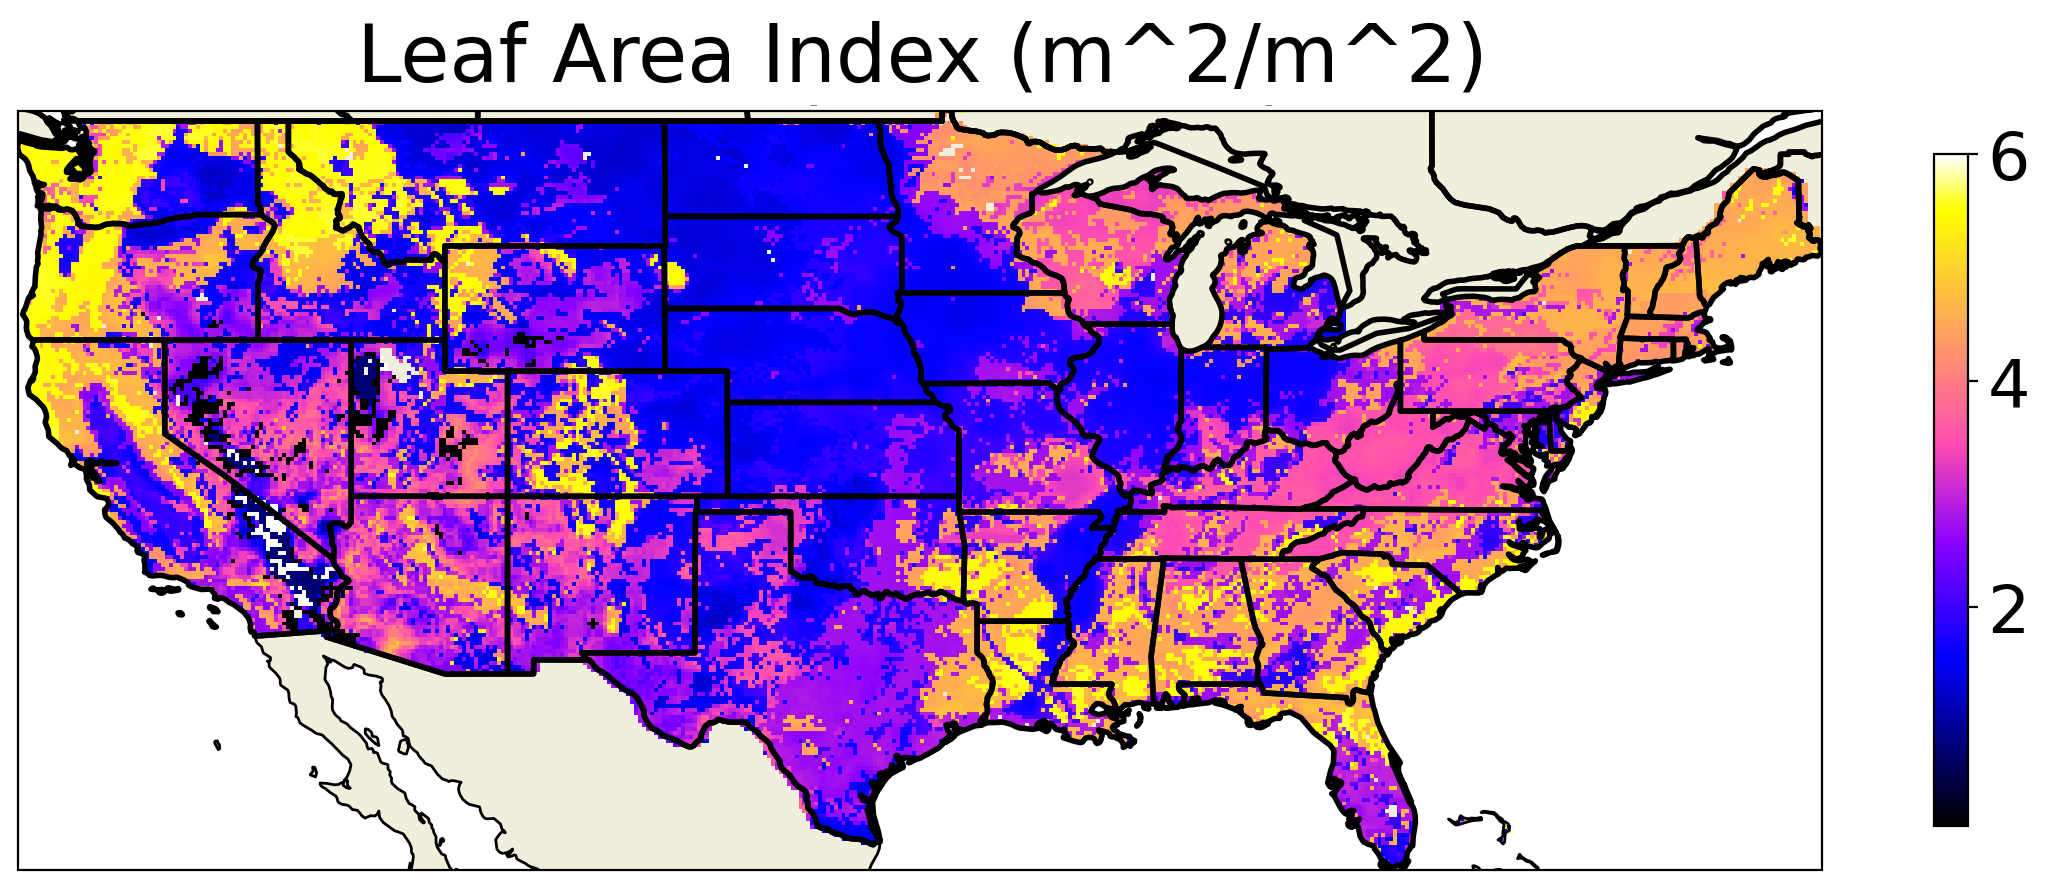
\includegraphics[width=.48\linewidth,draft=false]{figures/thesis-gridstats/gridstat-bulk_lai_2012-1_2023-12_y000-195_x000-462_mean.png}

    %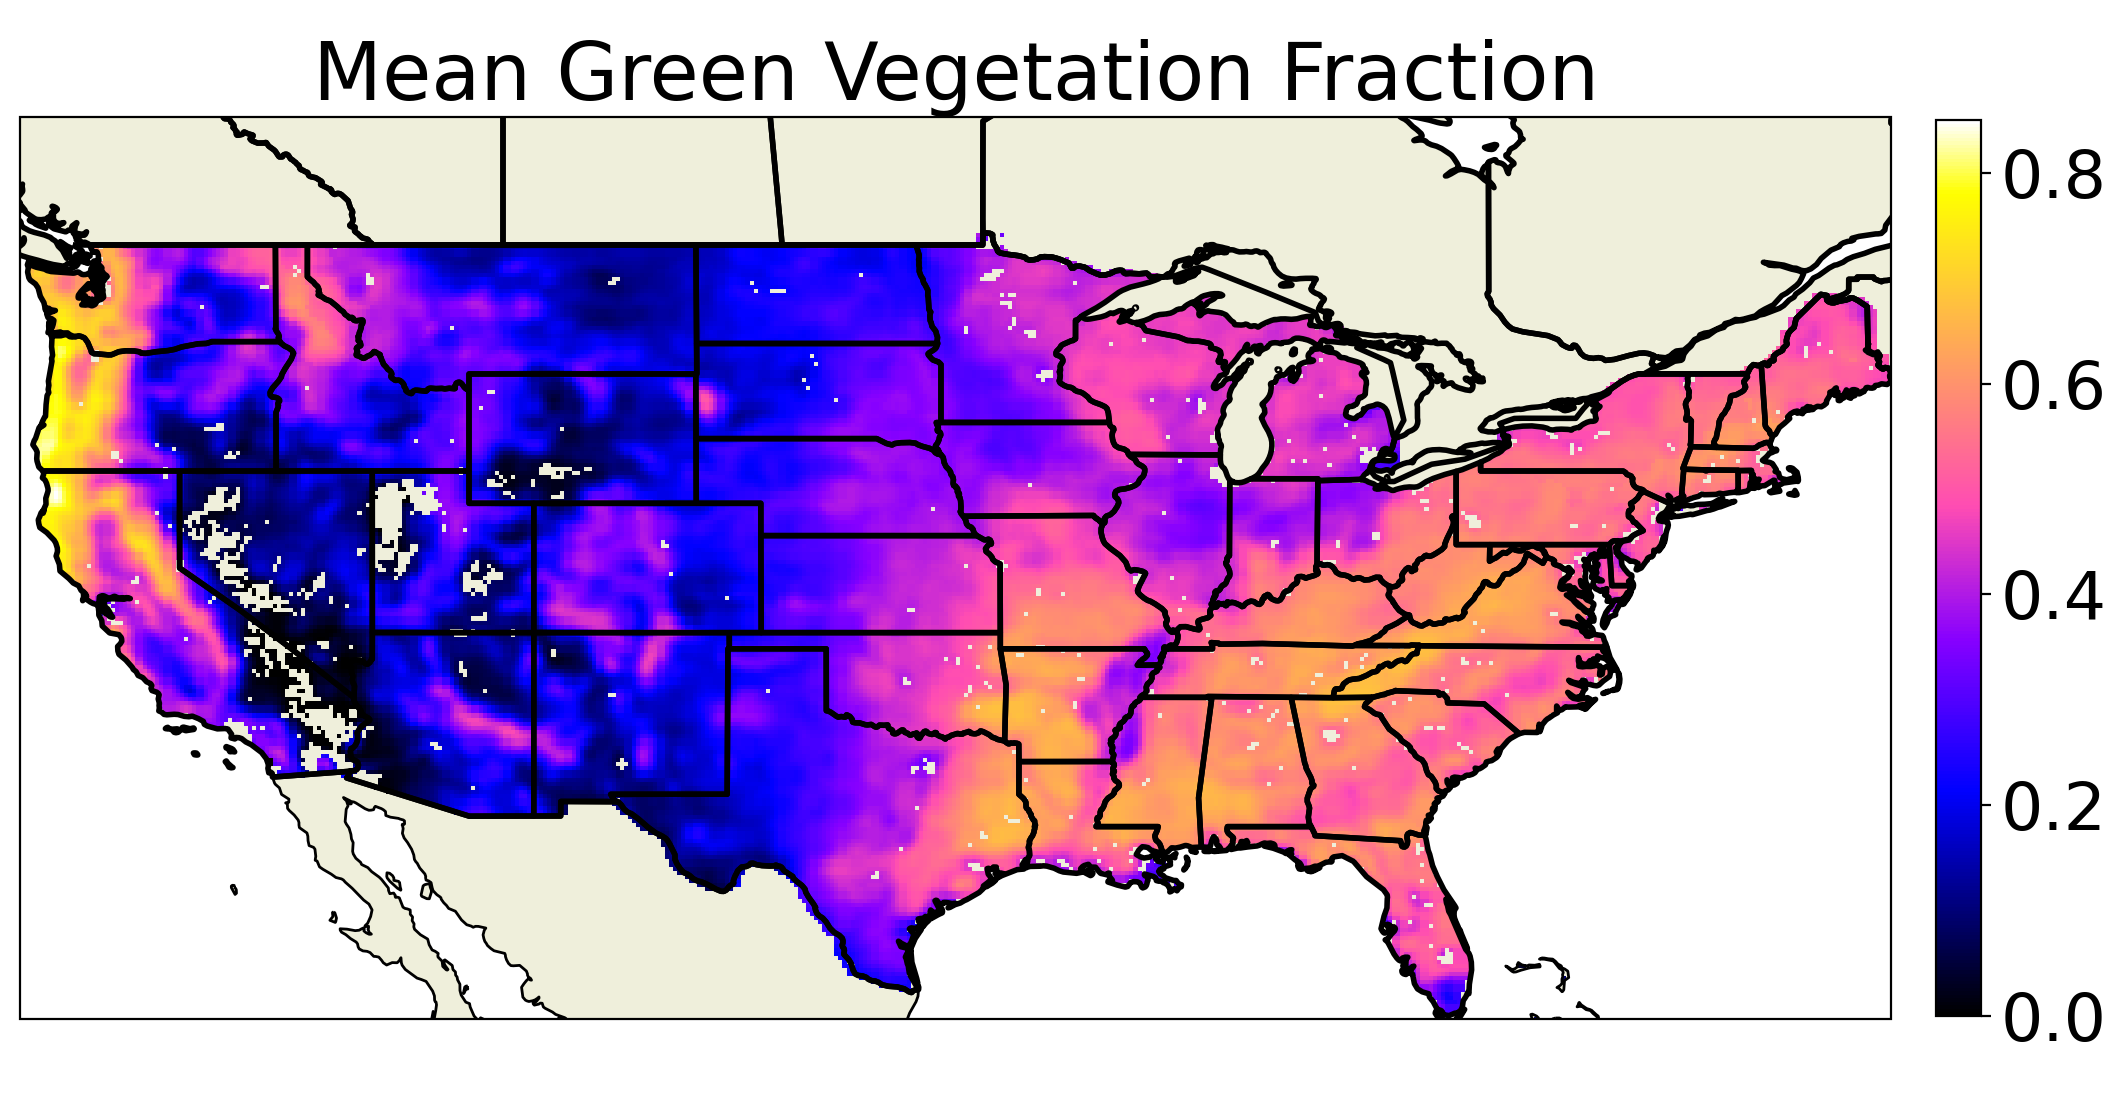
\includegraphics[width=.48\linewidth,draft=false]{figures/thesis-gridstats/gridstat-bulk_veg_2012-1_2023-12_y000-195_x000-462_mean.png}
    %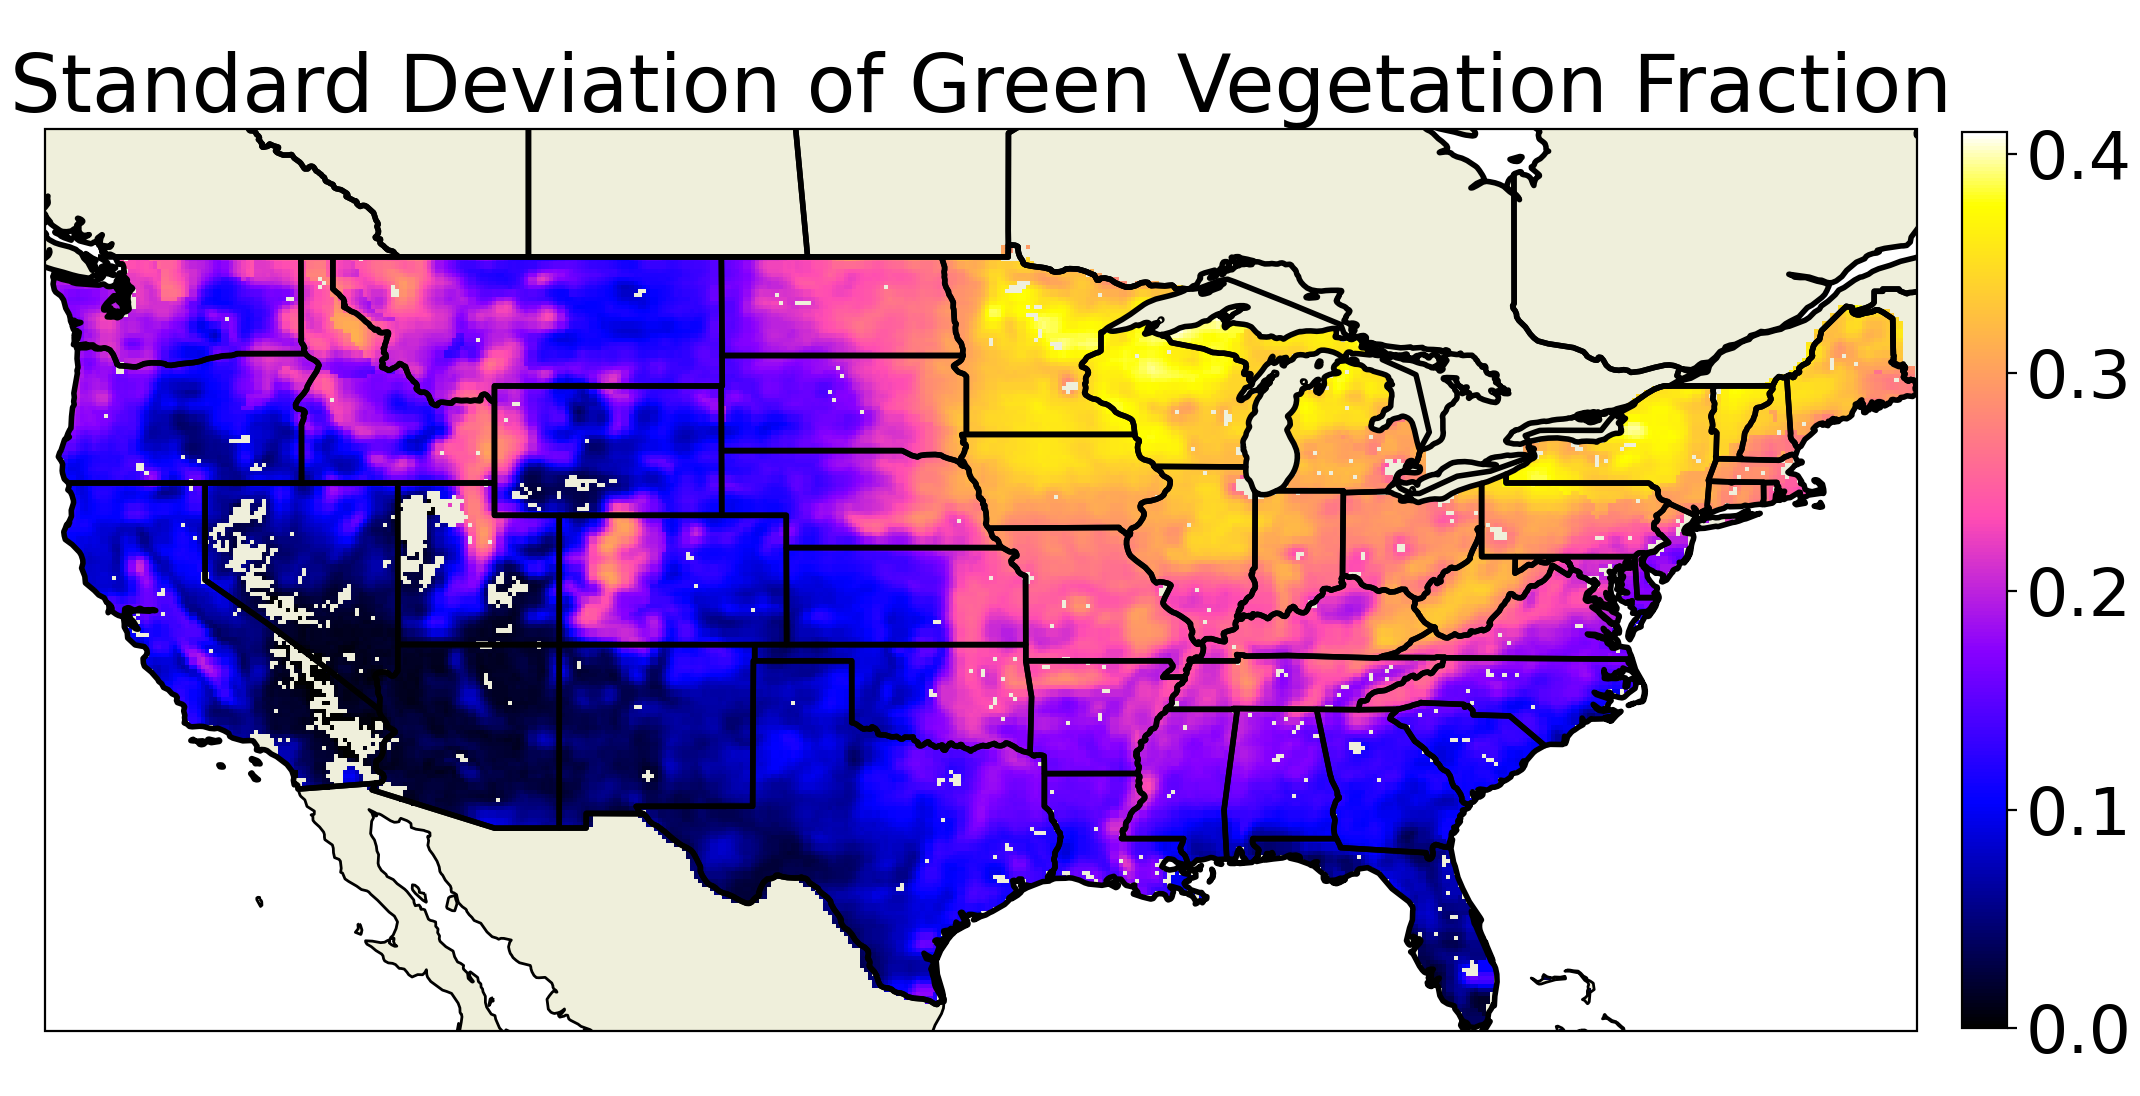
\includegraphics[width=.48\linewidth,draft=false]{figures/thesis-gridstats/gridstat-bulk_veg_2012-1_2023-12_y000-195_x000-462_stdev.png}
    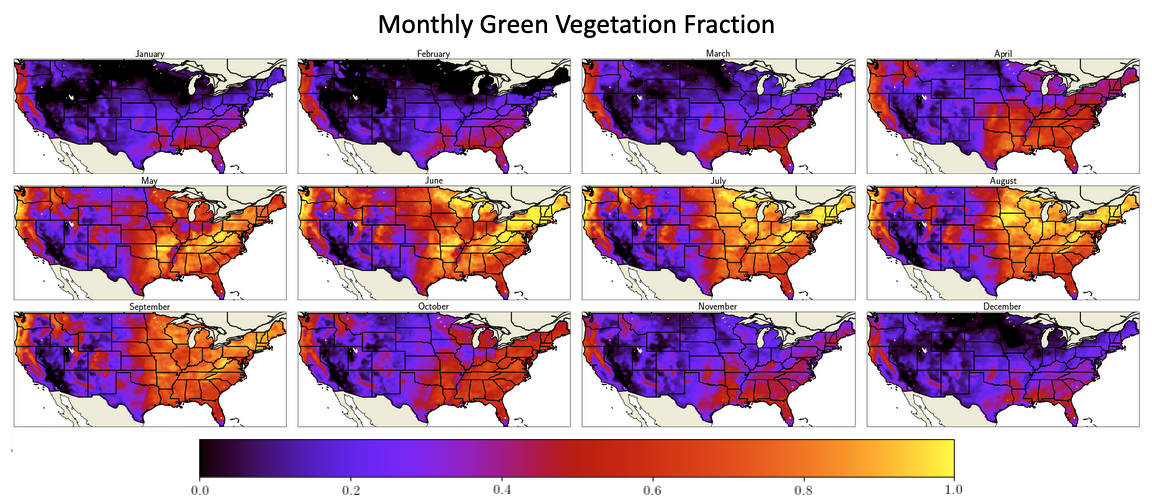
\includegraphics[width=.98\linewidth,draft=false]{figures/gvf/gvf_mosaic.png}

    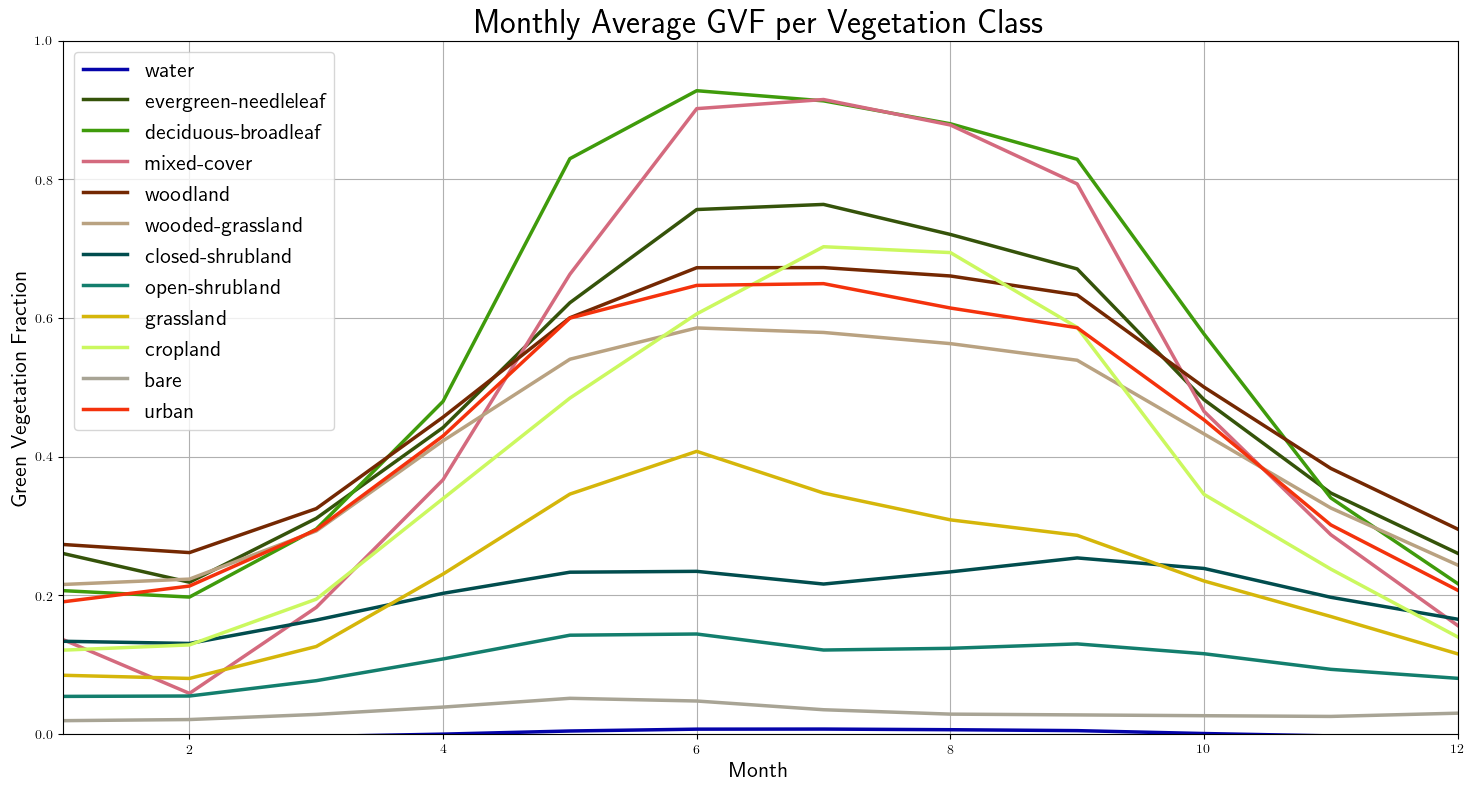
\includegraphics[width=.48\linewidth,draft=false]{figures/gvf/gvf_monthly_stats.png}
    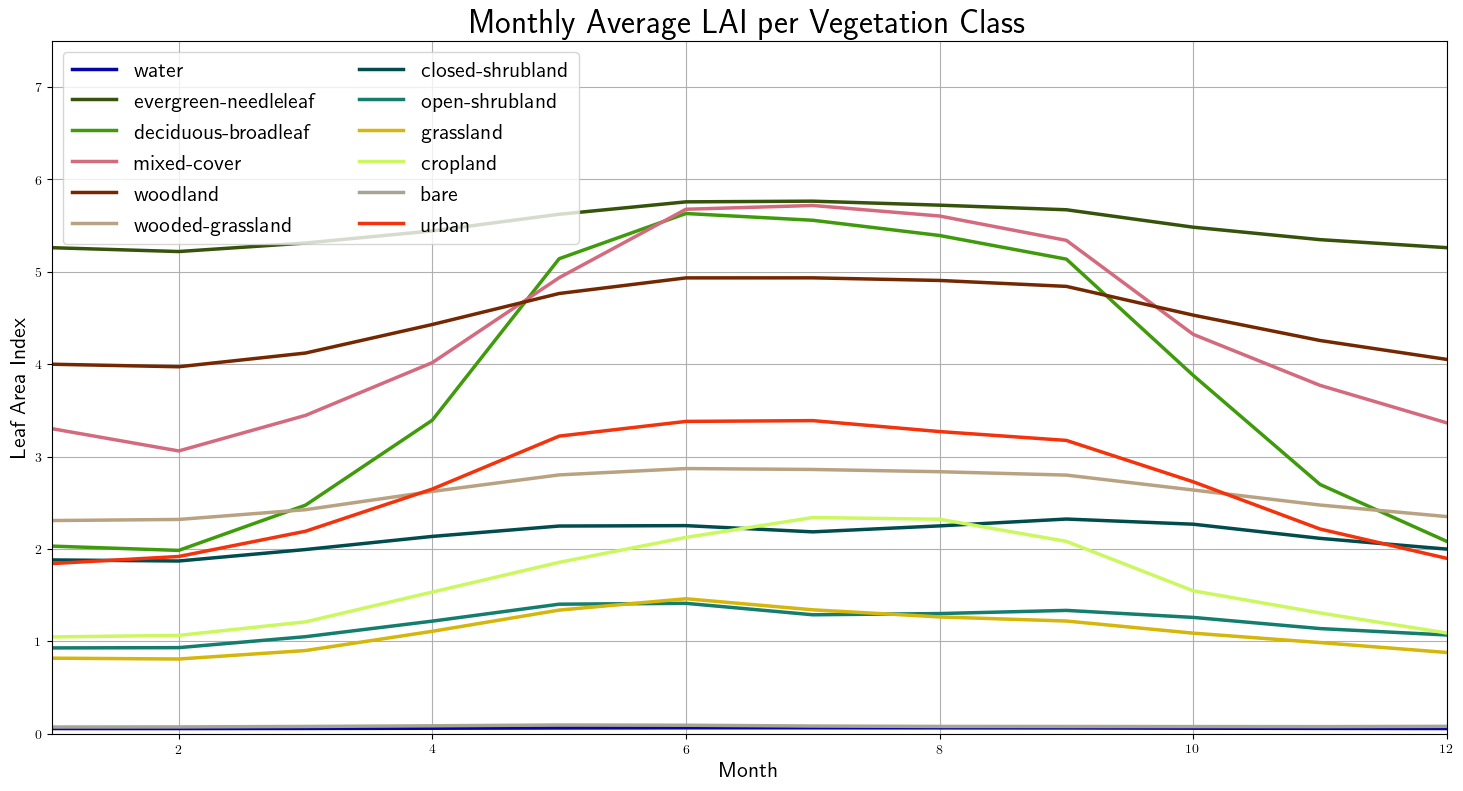
\includegraphics[width=.48\linewidth,draft=false]{figures/gvf/lai_monthly_stats.png}
    \caption{Monthly average green vegetation fraction (top), and monthly time series of GVF (bottom left) and LAI (bottom right) per vegetation class.}
    \label{gs-vegetation}
\end{figure}

%Although they vary smoothly on an hourly basis, the LAI and GVF parameters are similar to static parameters in that they cycle consistently per-pixel on an annual basis (rather than dynamically changing based on variable atmospheric conditions), and modulate the soil water dynamics via through their effect on the vegetation parameterization. As Figure \ref{gs-vegetation} indicates, the densest annual-averaged canopy cover corresponds to evergreen needleleaf surface types, and there is almost no canopy over croplands and grasslands of the Midwest, California Valley, and the Great Plains. The greenest satellite-derived vegetation covers the West Coast and Sierra ranges, followed by the South and Northeast. The standard deviation of GVF indicates the regions of most significant seasonal variability, which corresponds to deciduous-dominant locales.

Although they vary smoothly on an hourly basis, the LAI and GVF parameters are similar to static parameters in that they cycle consistently per-pixel on an annual basis (rather than dynamically changing based on variable atmospheric conditions), and modulate the soil water dynamics via through their effect on the vegetation parameterization. Figure \ref{gs-vegetation} displays the monthly GVF averages retrieved by \parencite{gutman_derivation_1998}, which have a substantial influence on the magnitude of plant transpiration. As defined in \parencite{wei_improvement_2011}, the GVF directly scales the plant transpiration as a multiplicative coefficient, and also modulates the LAI between a minimum and maximum value that are uniquely specified for each surface category.

\begin{figure}[h!]
    \centering
    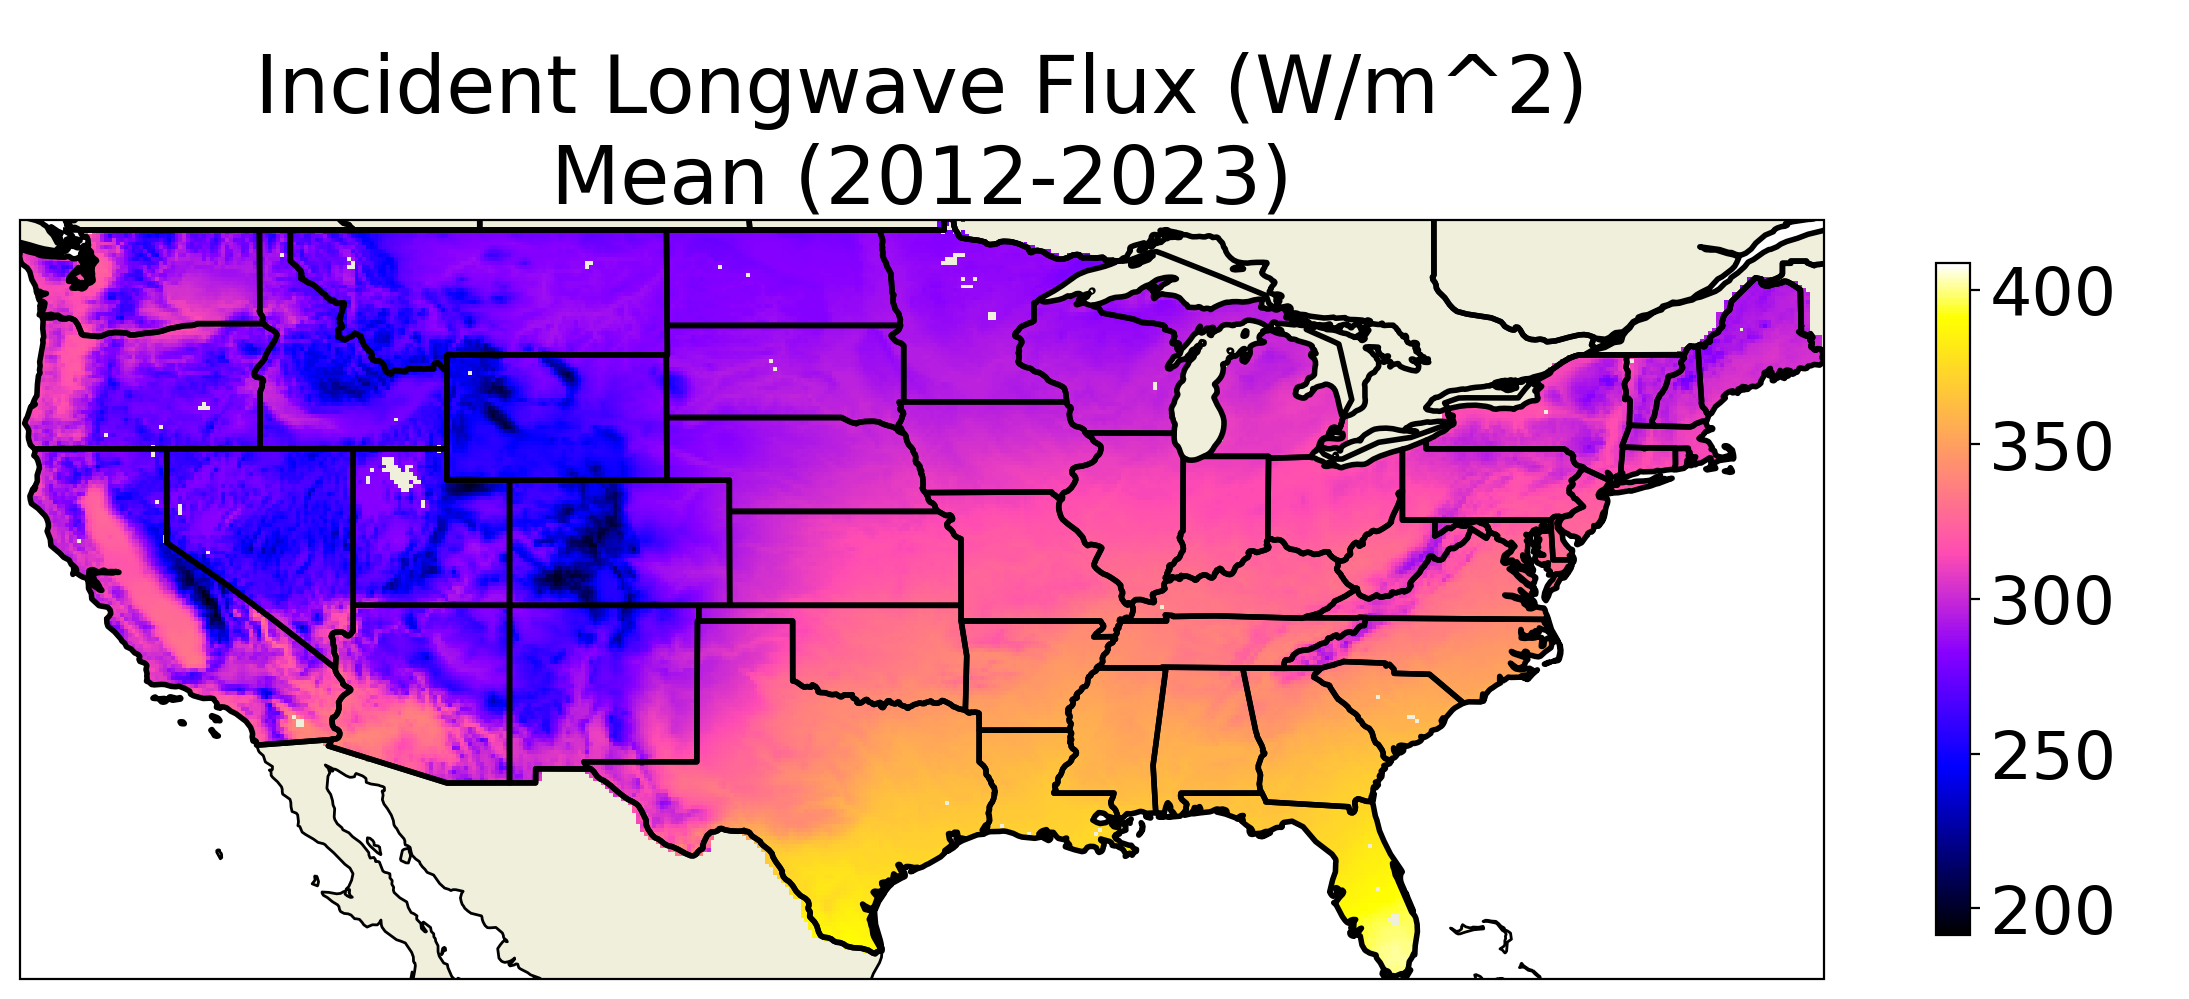
\includegraphics[width=.48\linewidth,draft=false]{figures/thesis-gridstats/gridstat-bulk_dlwrf_2012-1_2023-12_y000-195_x000-462_mean.png}
    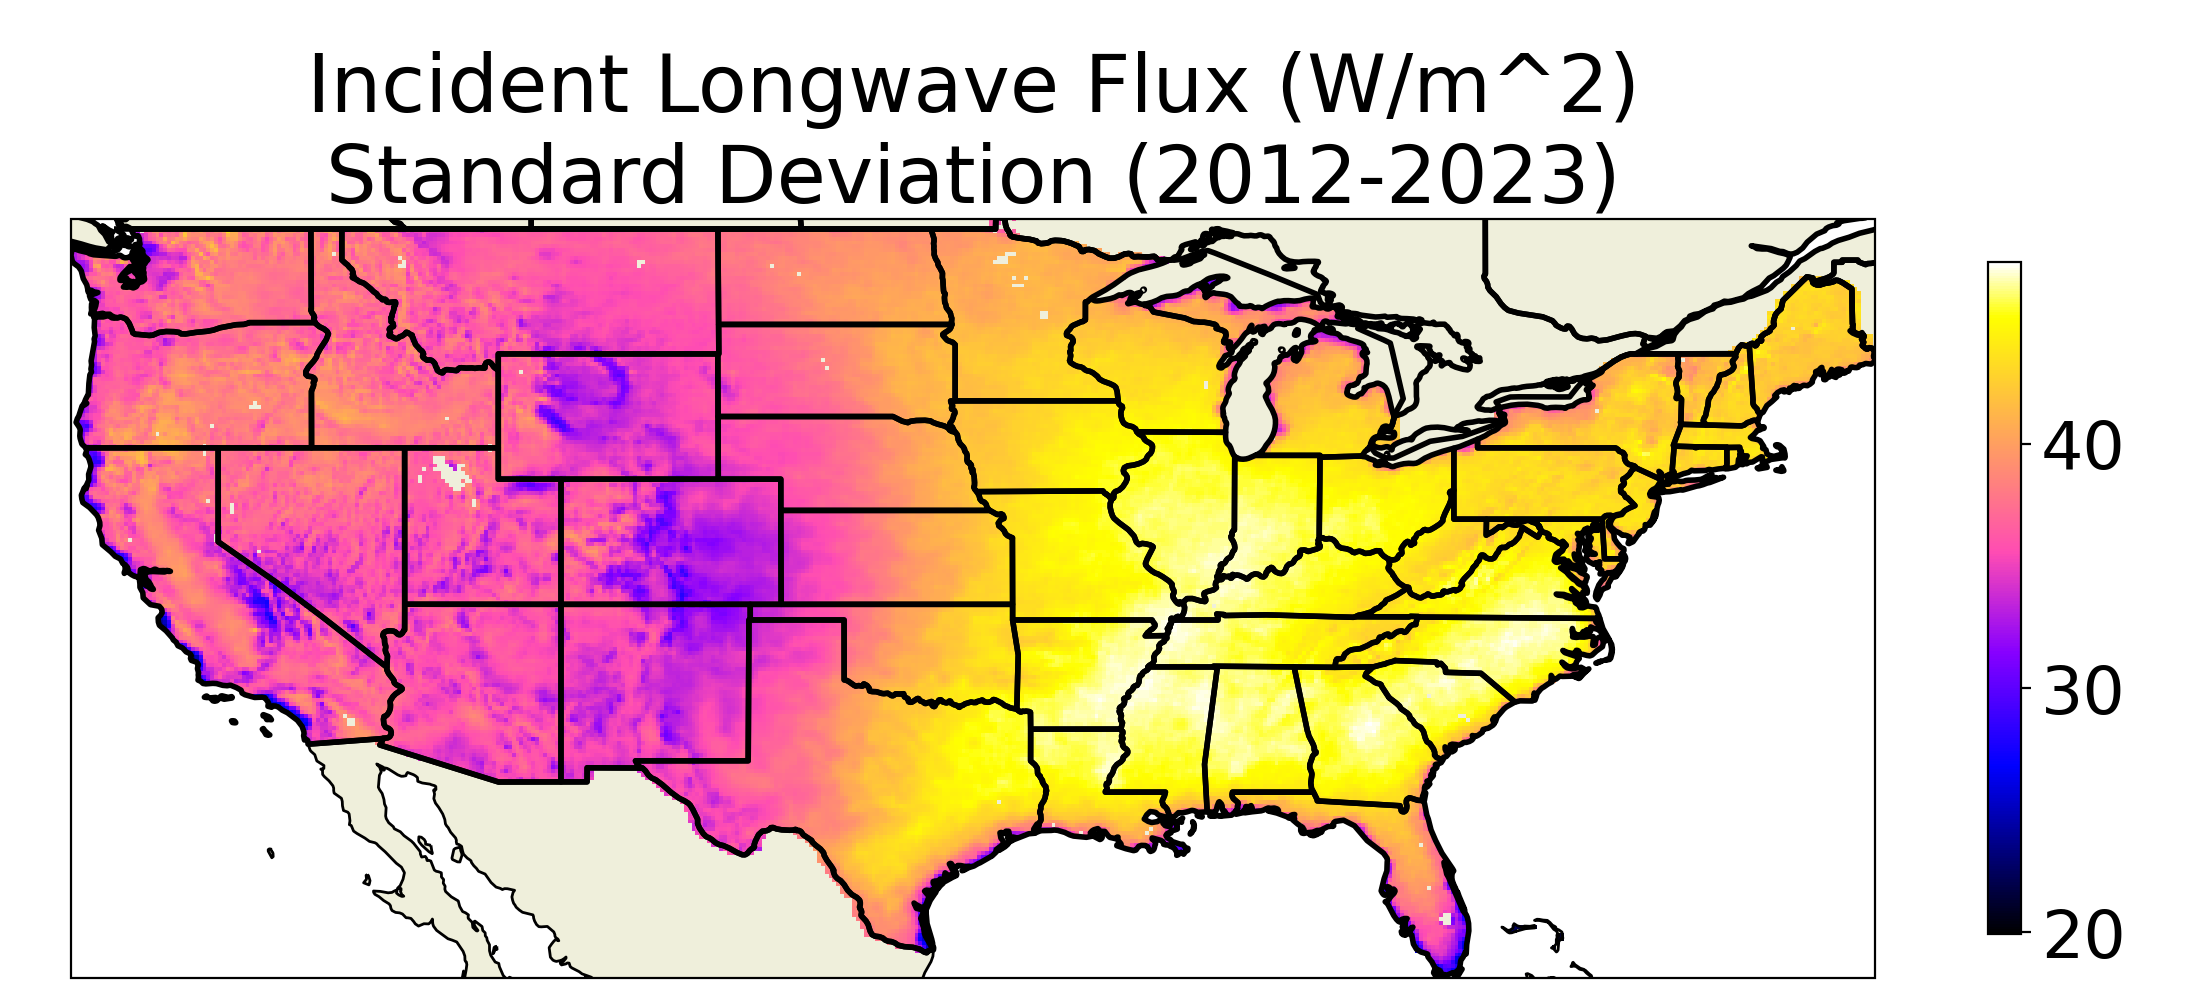
\includegraphics[width=.48\linewidth,draft=false]{figures/thesis-gridstats/gridstat-bulk_dlwrf_2012-1_2023-12_y000-195_x000-462_stdev.png}

    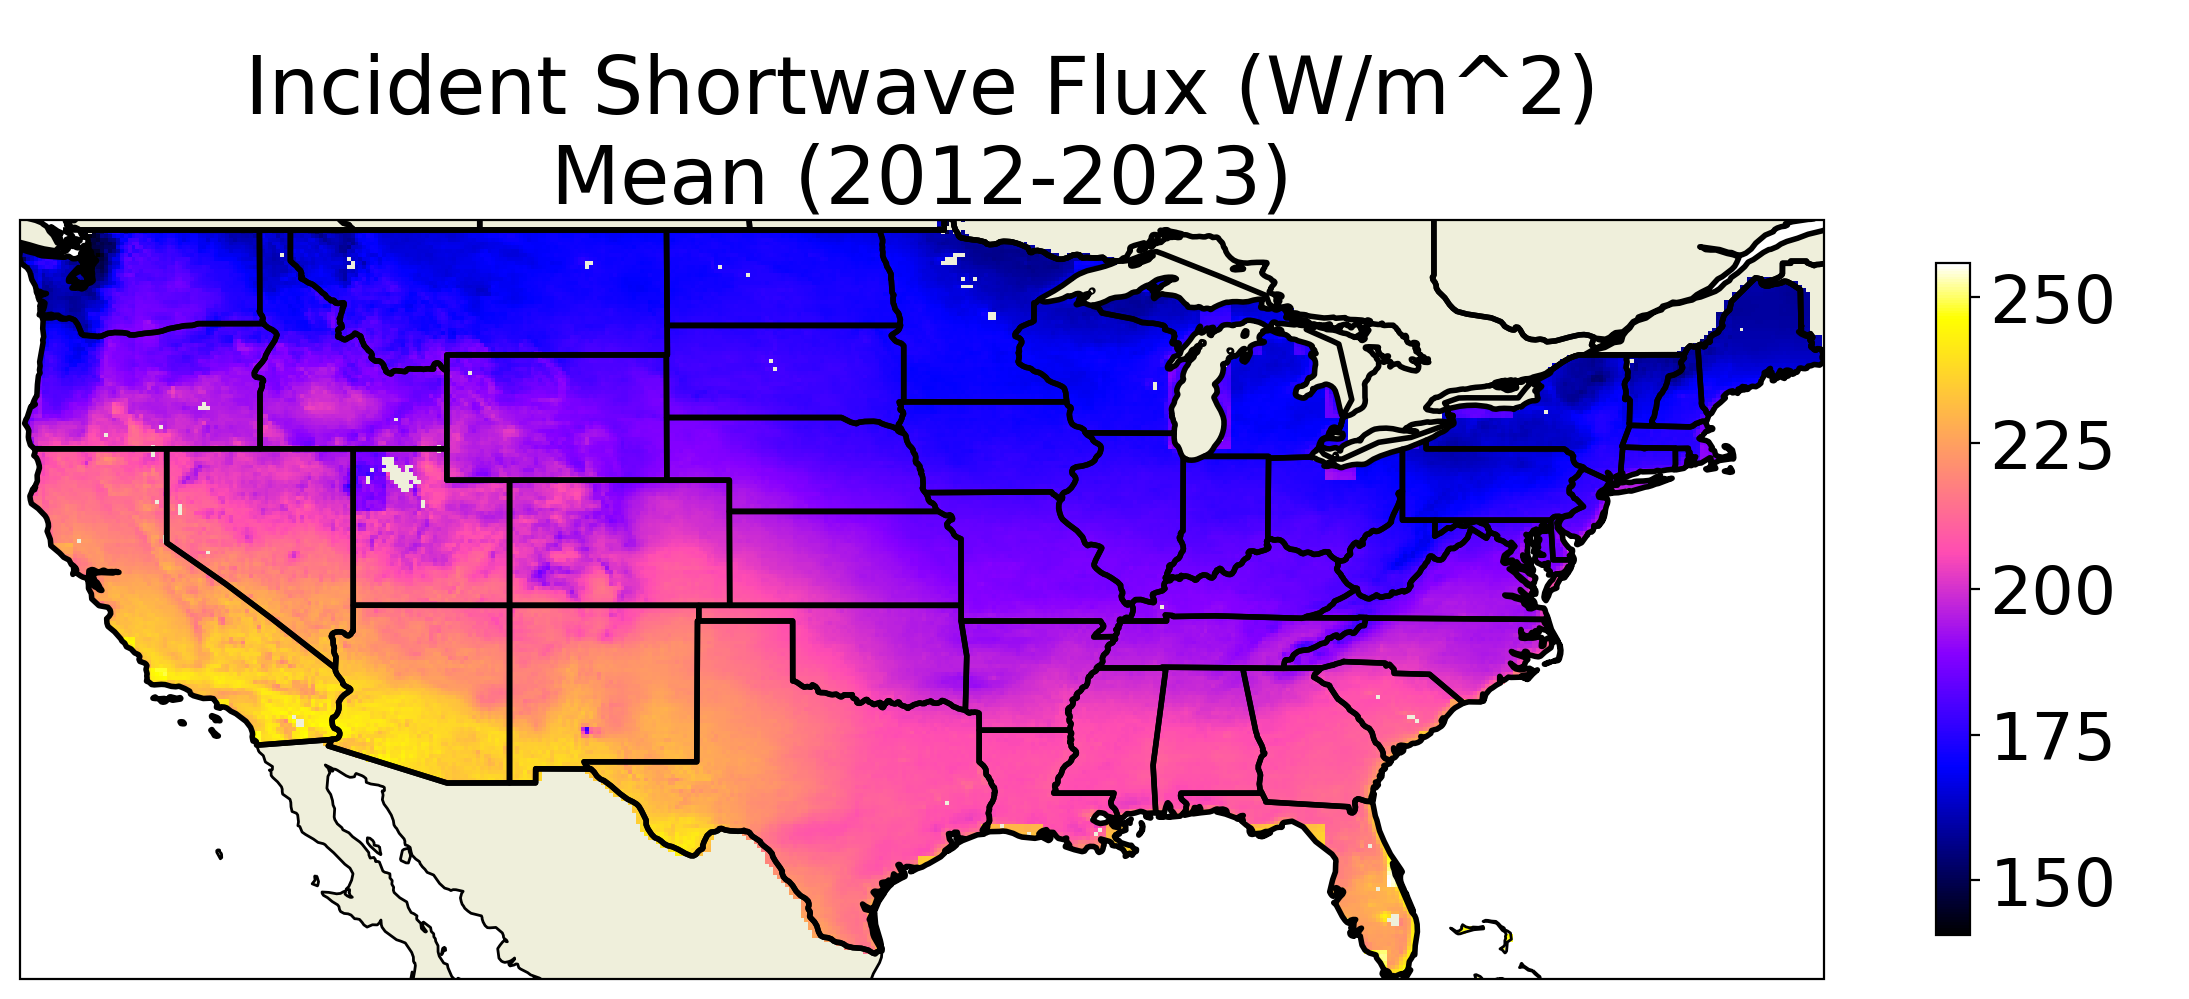
\includegraphics[width=.48\linewidth,draft=false]{figures/thesis-gridstats/gridstat-bulk_dswrf_2012-1_2023-12_y000-195_x000-462_mean.png}
    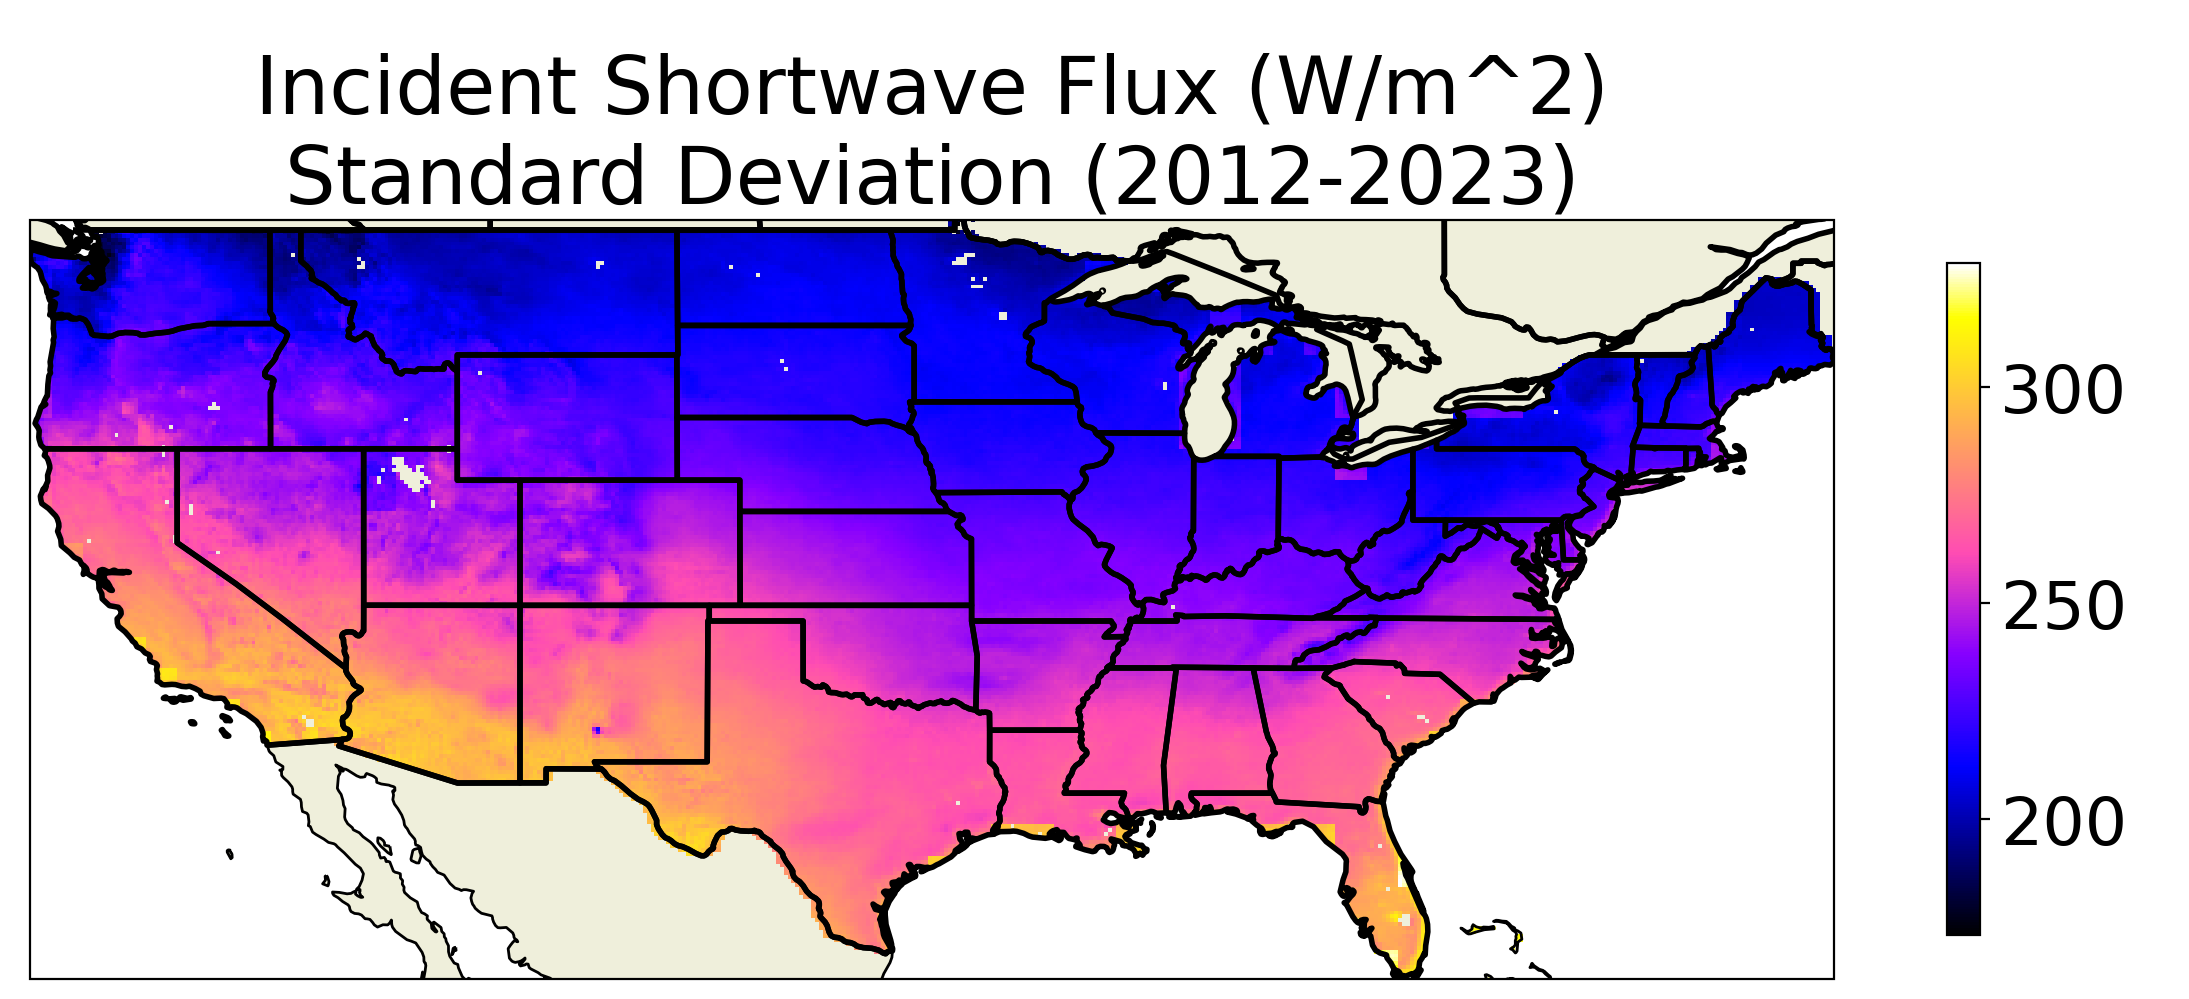
\includegraphics[width=.48\linewidth,draft=false]{figures/thesis-gridstats/gridstat-bulk_dswrf_2012-1_2023-12_y000-195_x000-462_stdev.png}
    \caption{Gridded mean and standard deviation of radiative forcings (2012-2023).}
    \label{gs-radiative}
\end{figure}

In addition to the substantial regional variability of the static parameterization of Noah-LSM, there are considerable regional and seasonal differences in the NLDAS-2 atmospheric forcing time series. Figure \ref{gs-radiative} shows the mean and standard deviation of radiative features over the full spatial and temporal domain, which demonstrates the distribution of annually-averaged downwelling radiation. Feedback from terrestrial emissions mean that longwave radiation is highest in regions that are generally cloudier, have warmer land surface temperatures, and are lower in elevation. The shortwave flux is highest at lower latitudes due to Earth's axial tilt, and in arid regions where there are fewer clouds.

\begin{figure}[hp!]
    \centering
    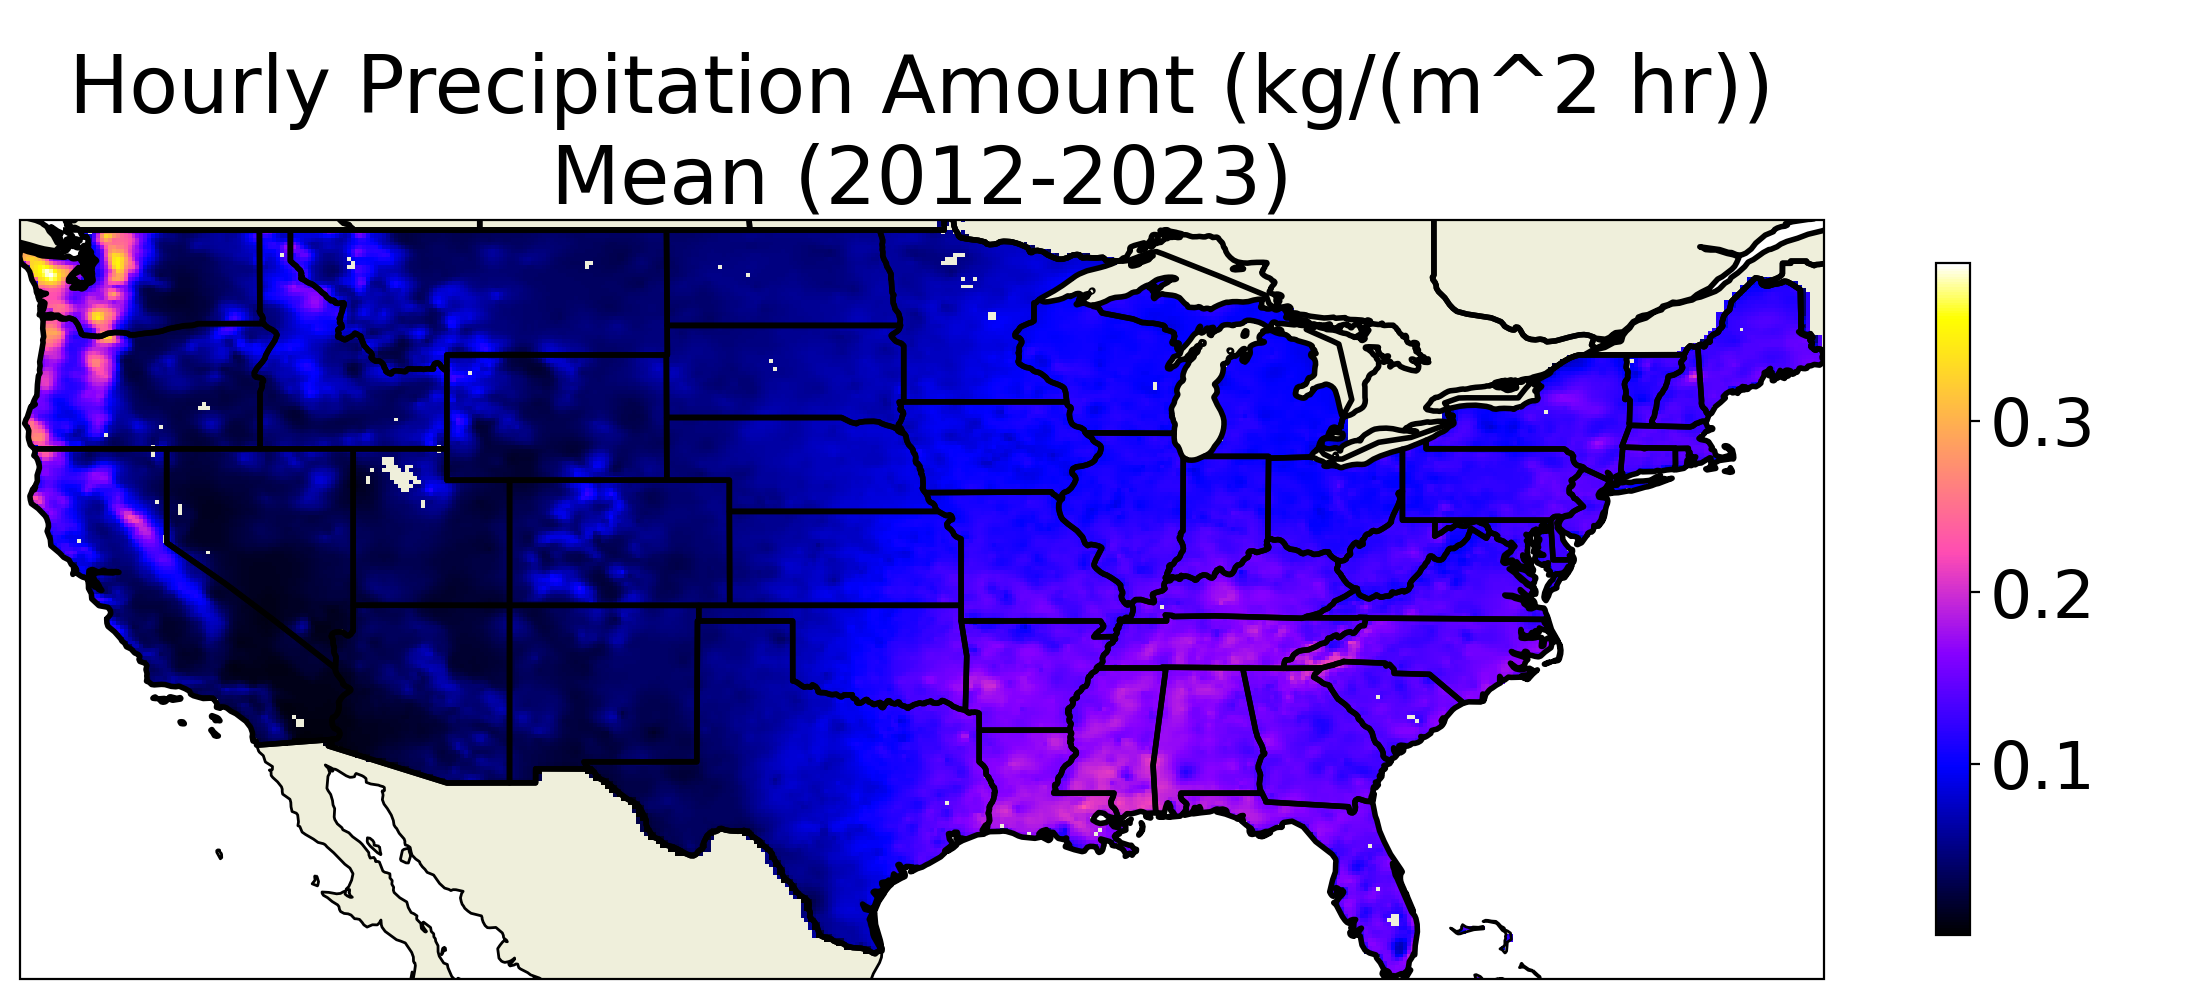
\includegraphics[width=.48\linewidth]{figures/thesis-gridstats/gridstat-bulk_apcp_2012-1_2023-12_y000-195_x000-462_mean.png}
    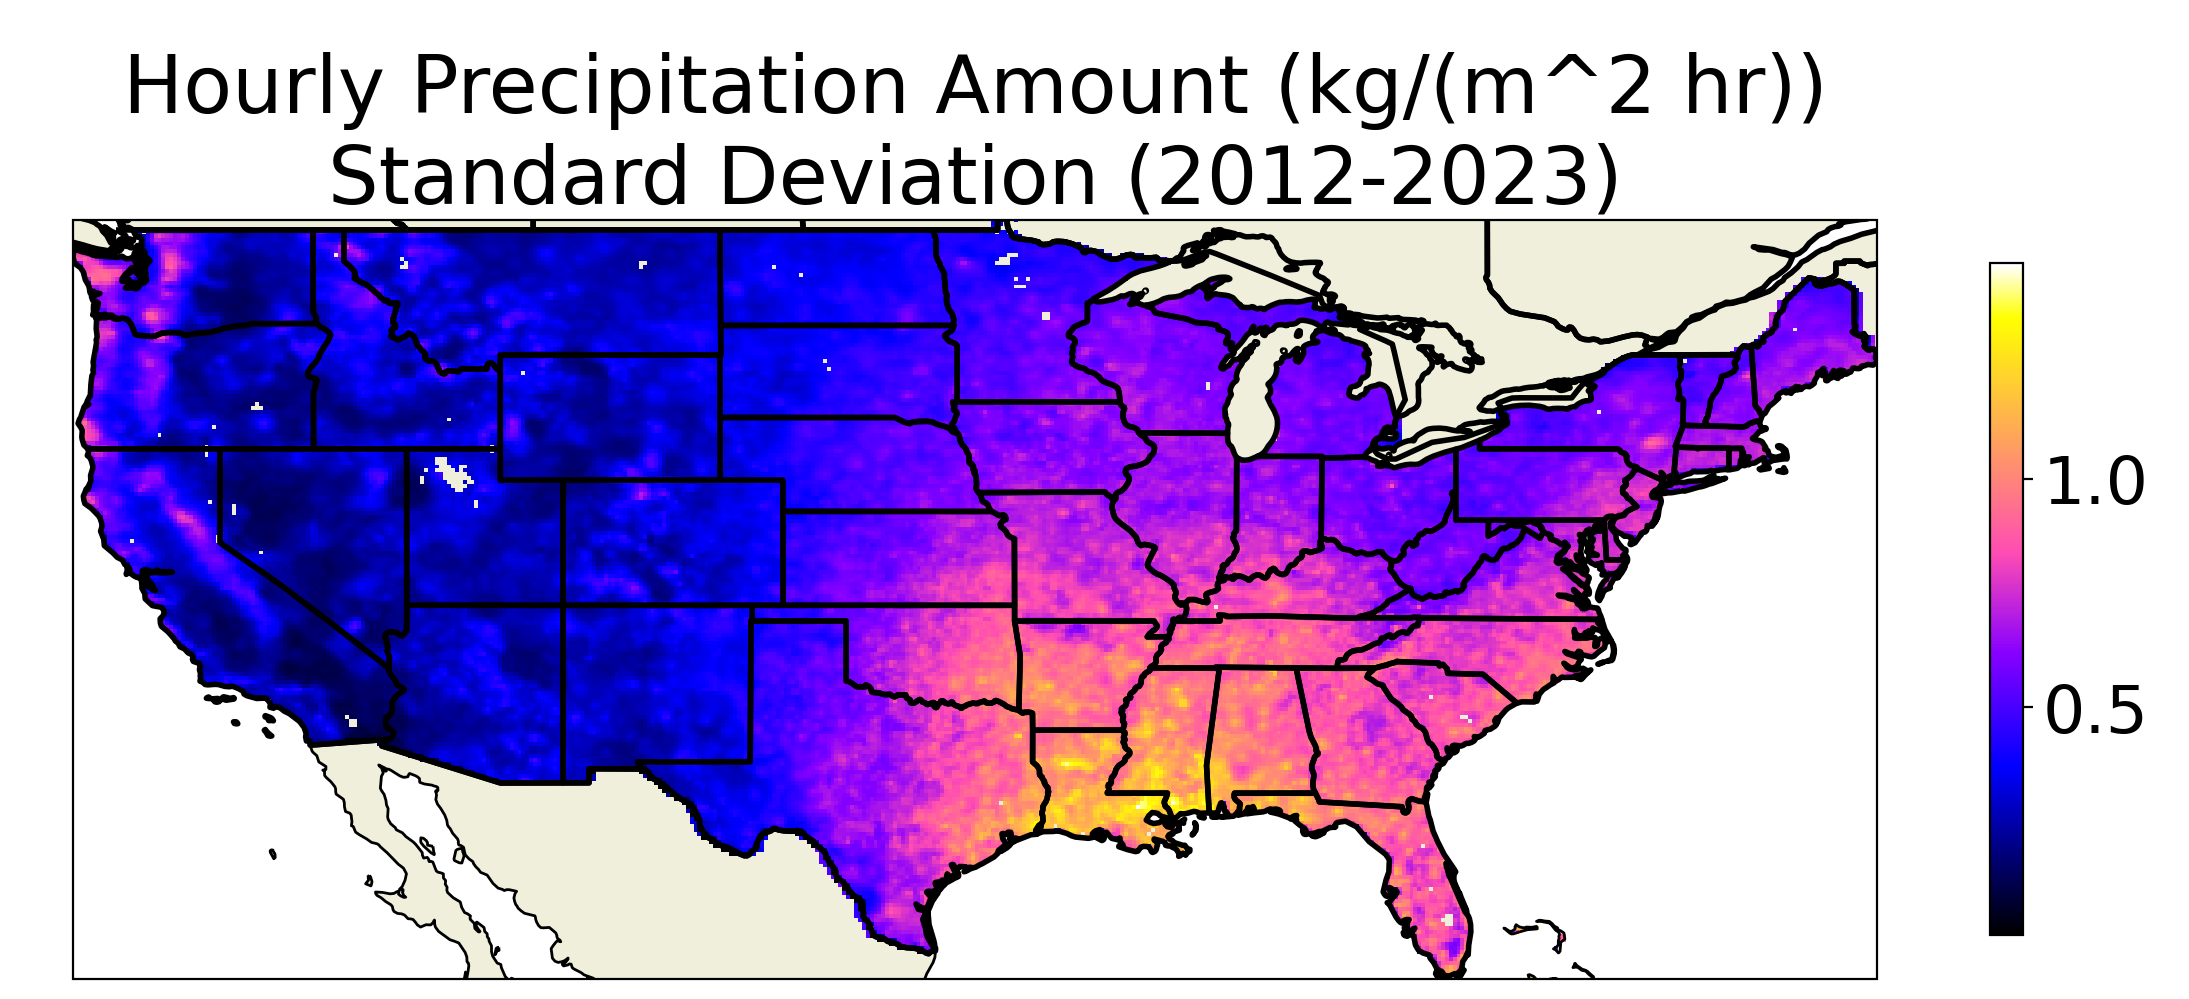
\includegraphics[width=.48\linewidth]{figures/thesis-gridstats/gridstat-bulk_apcp_2012-1_2023-12_y000-195_x000-462_stdev.png}

    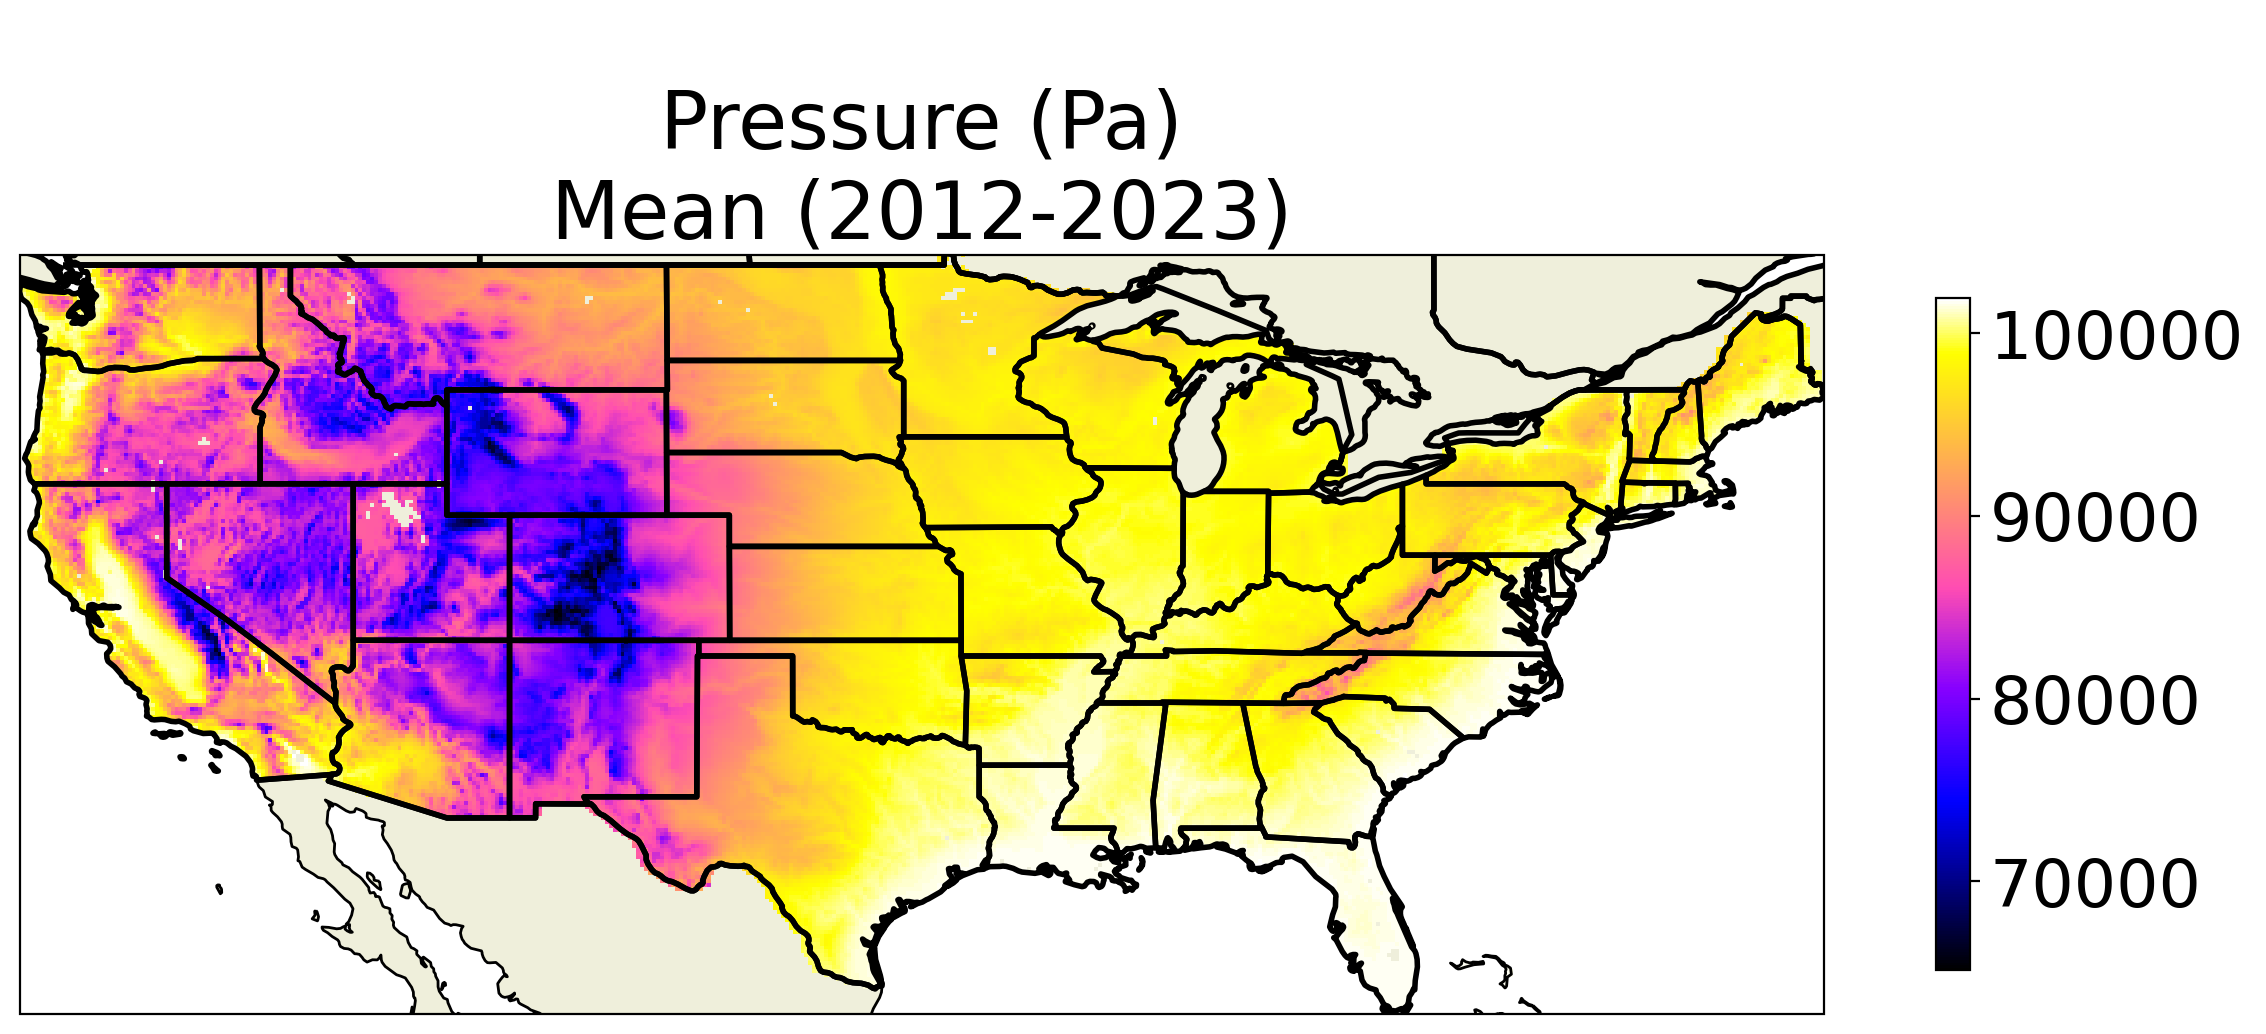
\includegraphics[width=.48\linewidth]{figures/thesis-gridstats/gridstat-bulk_pres_2012-1_2023-12_y000-195_x000-462_mean.png}
    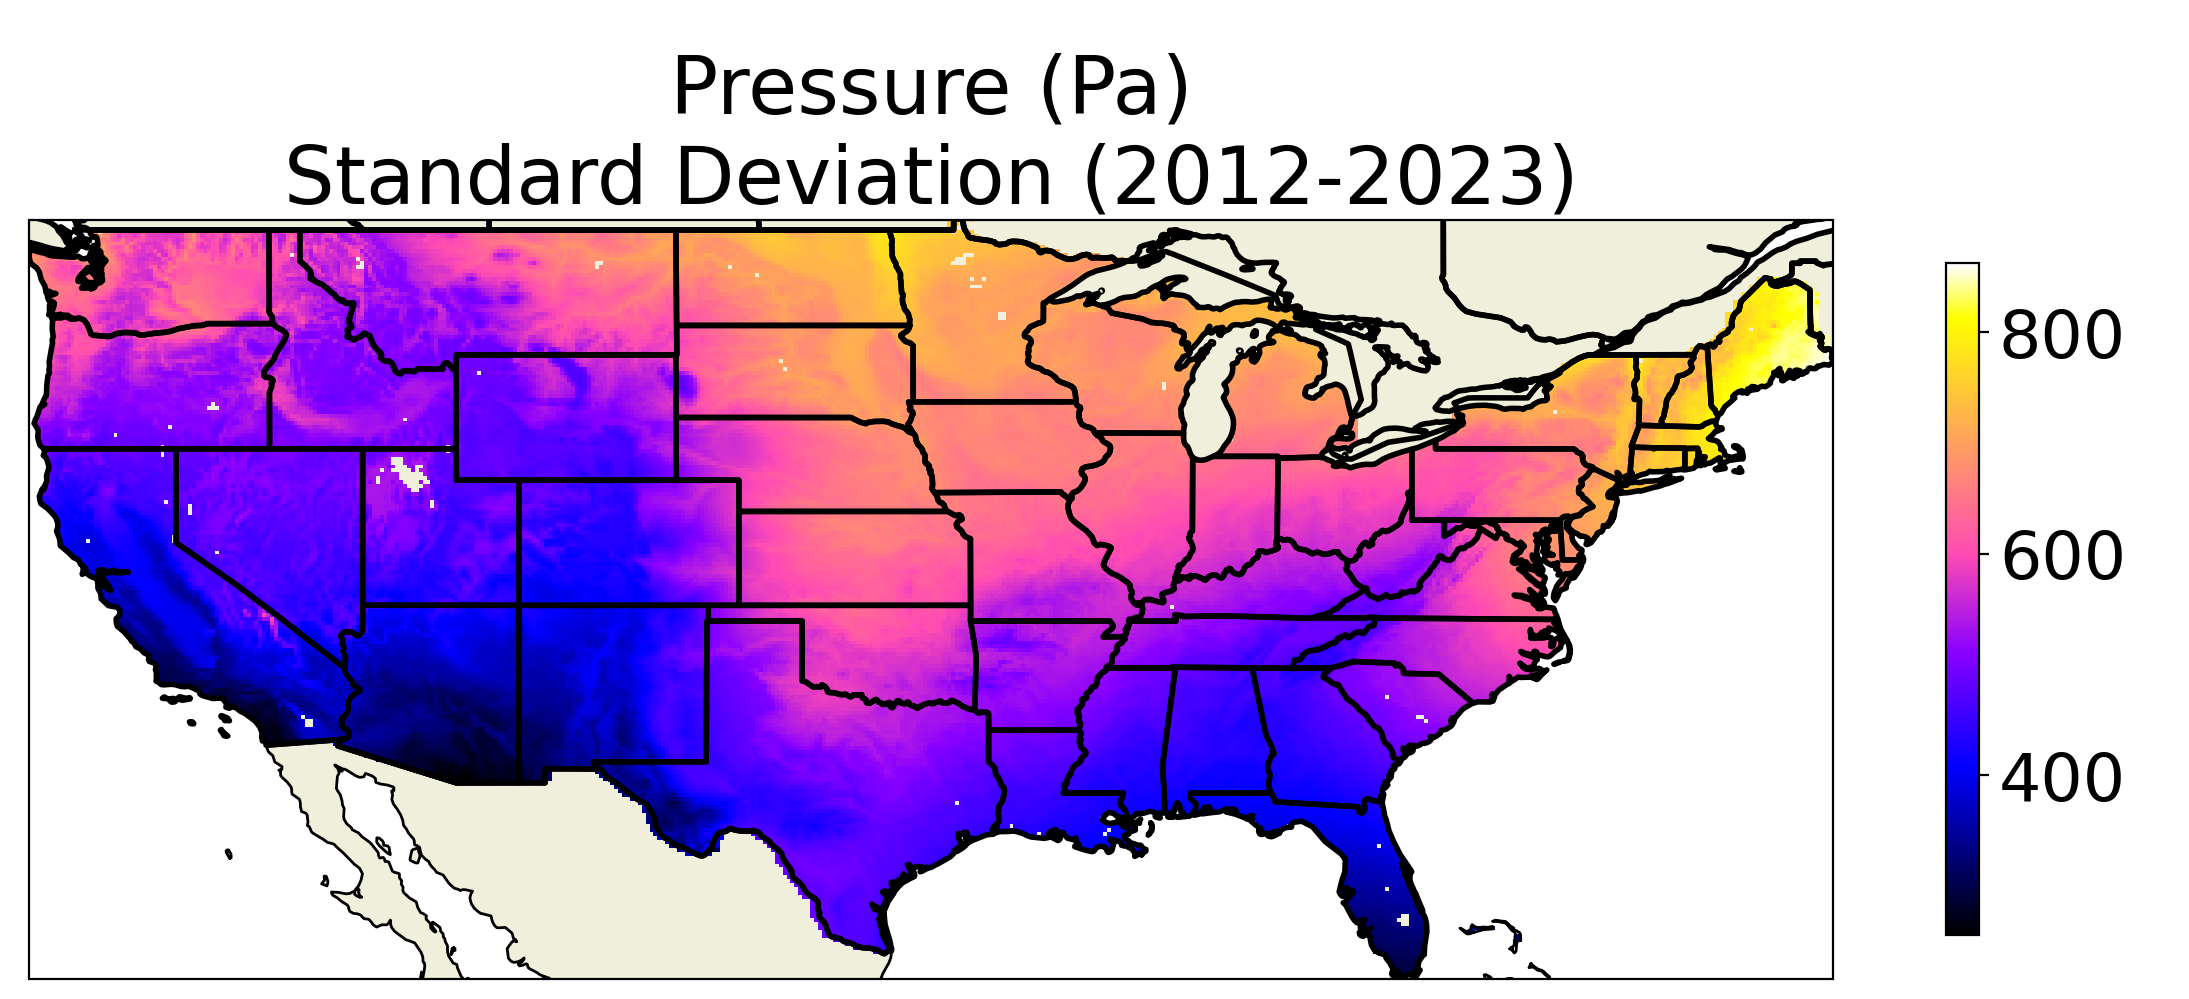
\includegraphics[width=.48\linewidth]{figures/thesis-gridstats/gridstat-bulk_pres_2012-1_2023-12_y000-195_x000-462_stdev.png}

    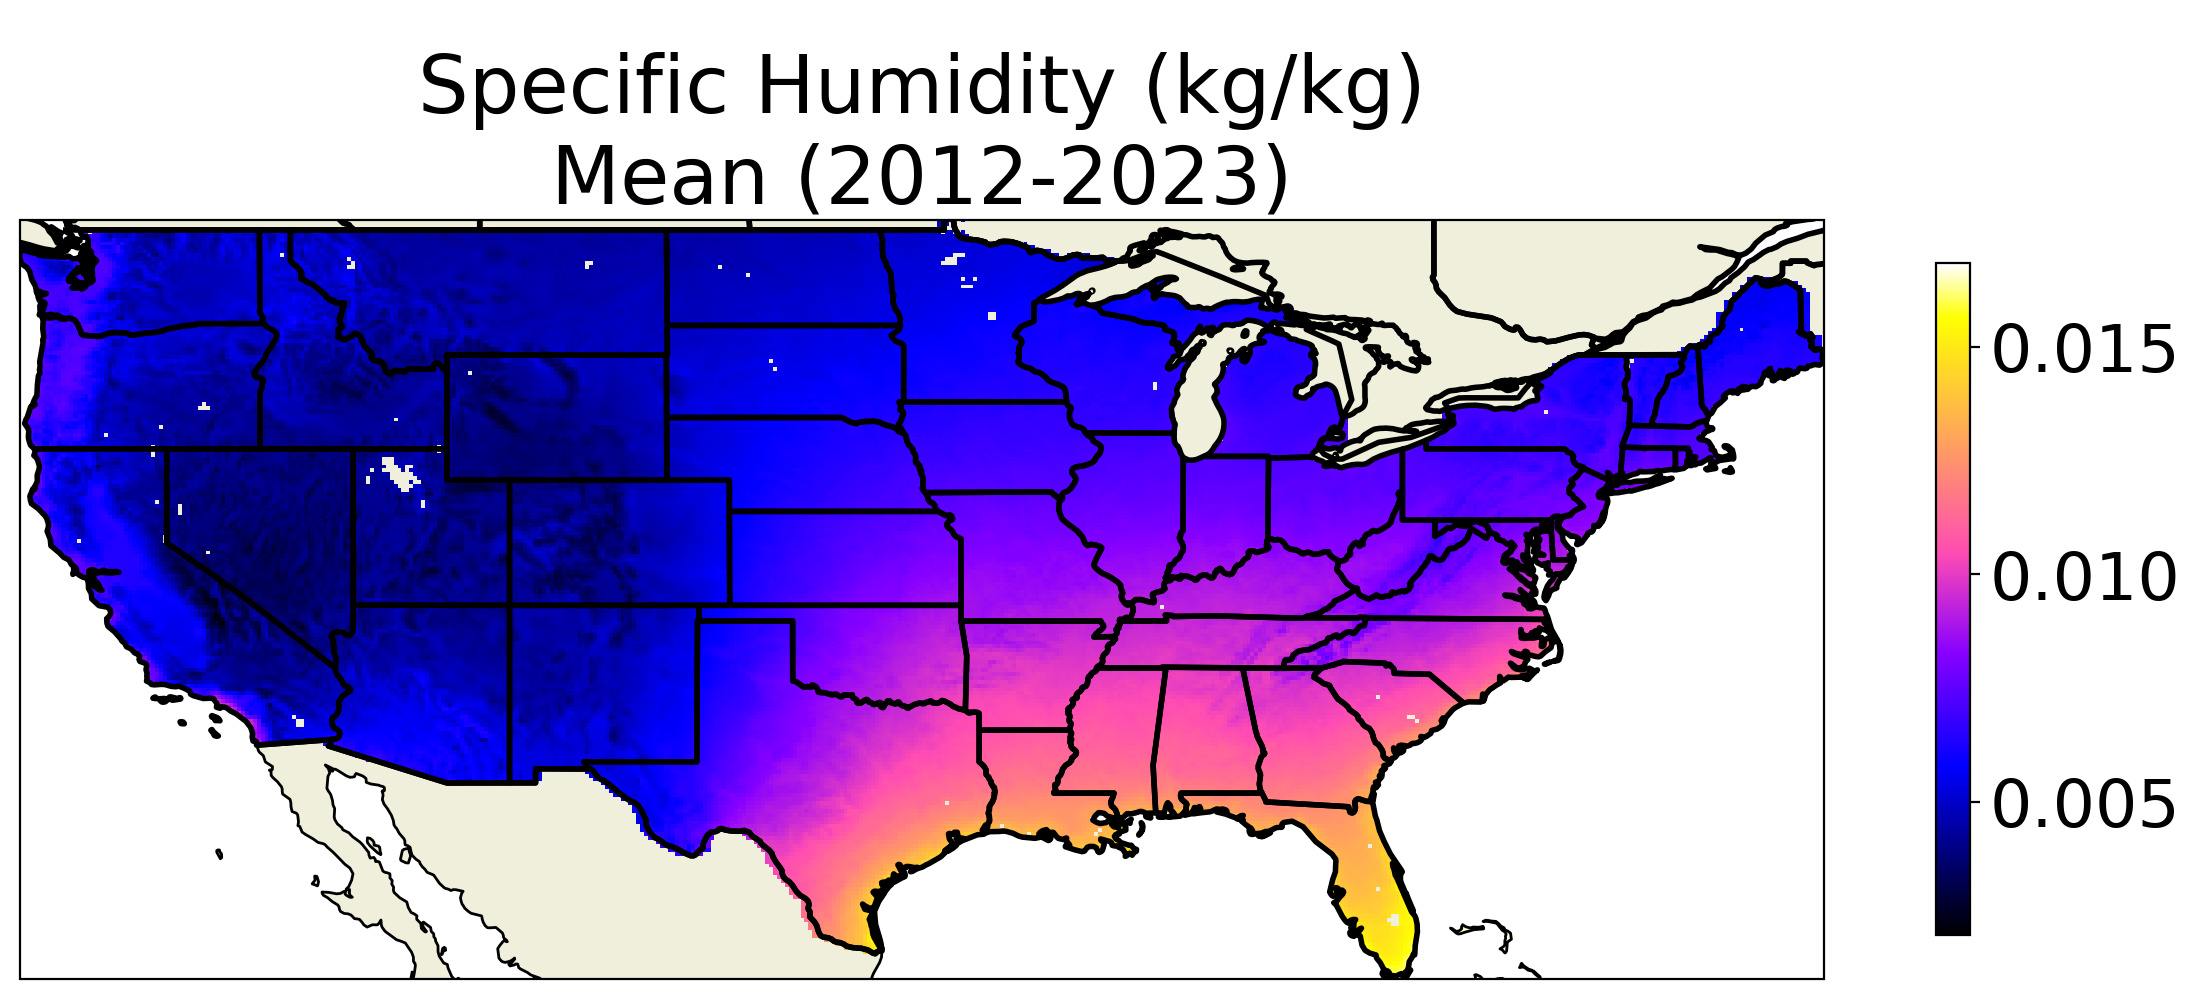
\includegraphics[width=.48\linewidth]{figures/thesis-gridstats/gridstat-bulk_spfh_2012-1_2023-12_y000-195_x000-462_mean.png}
    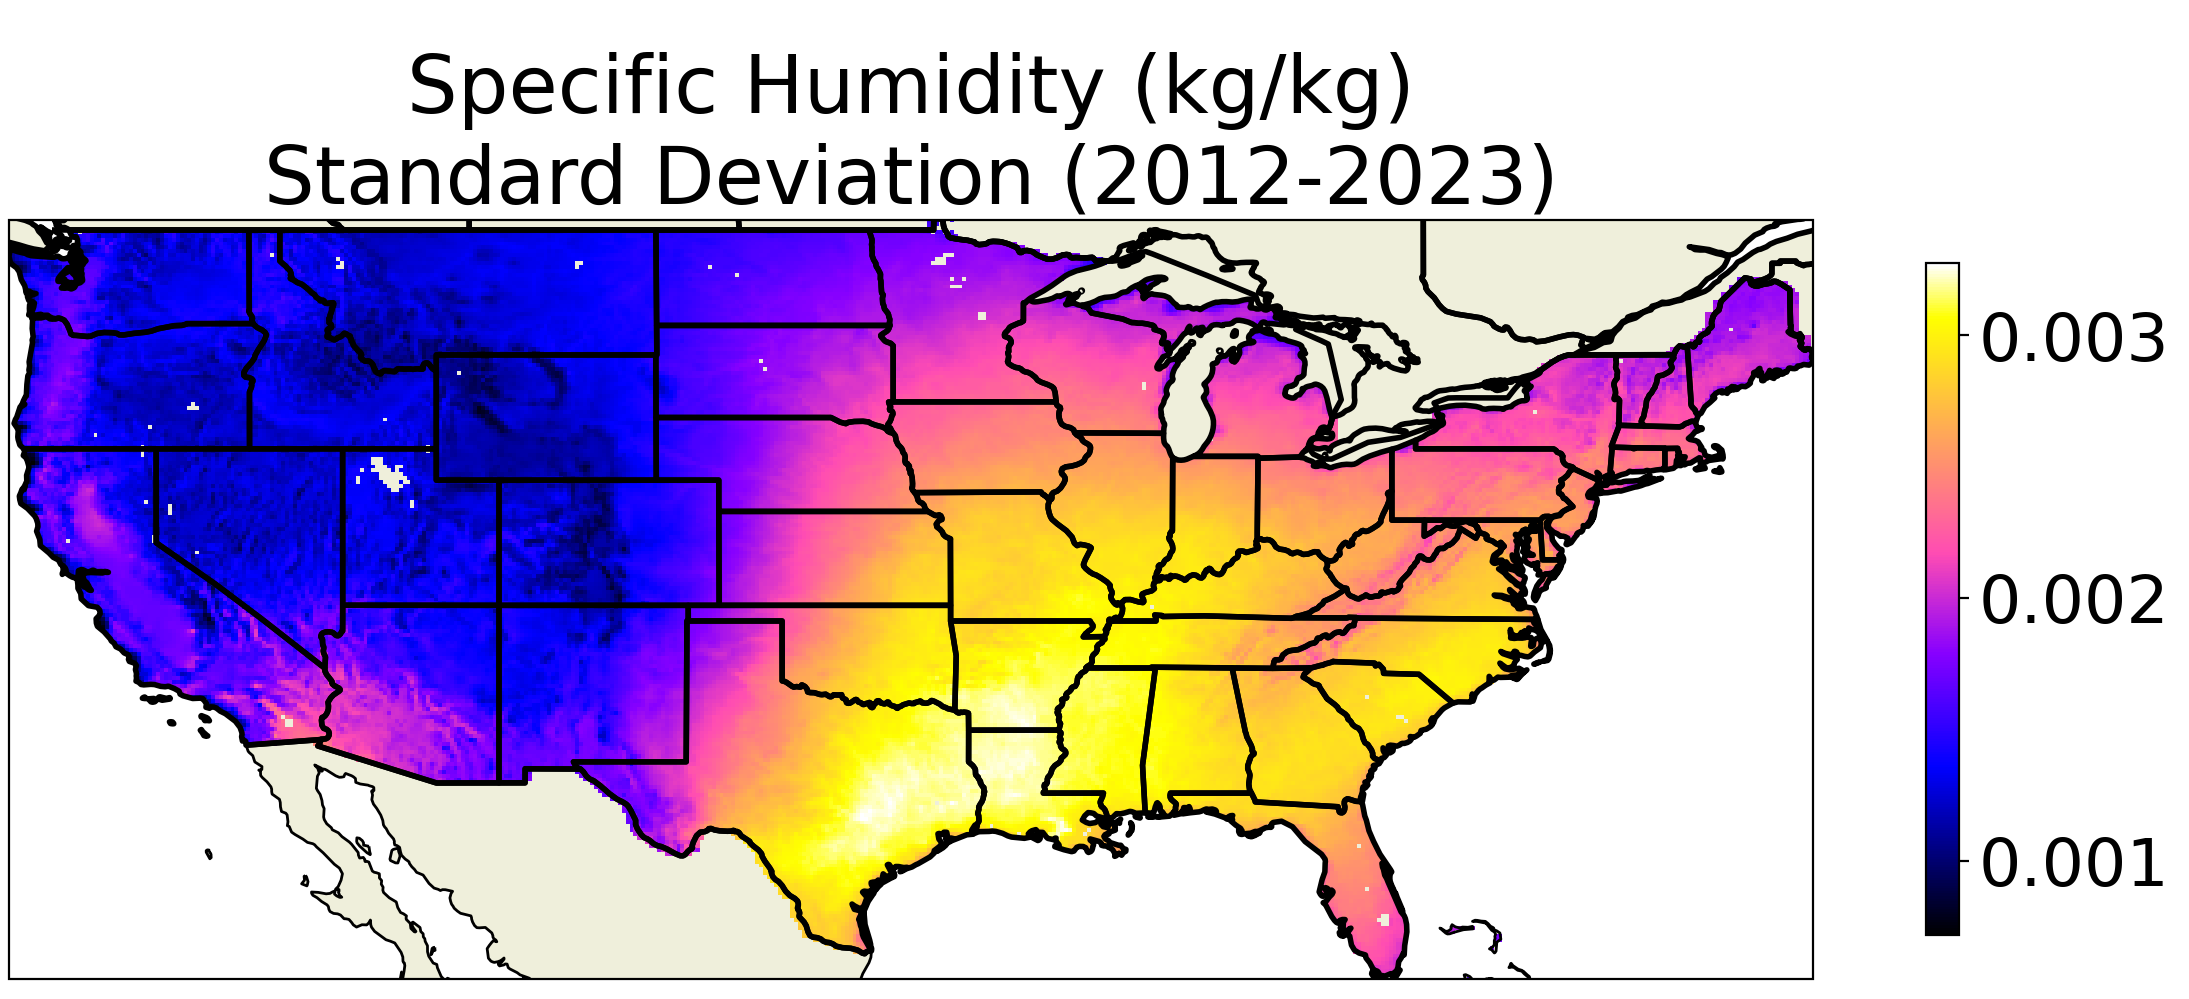
\includegraphics[width=.48\linewidth]{figures/thesis-gridstats/gridstat-bulk_spfh_2012-1_2023-12_y000-195_x000-462_stdev.png}

    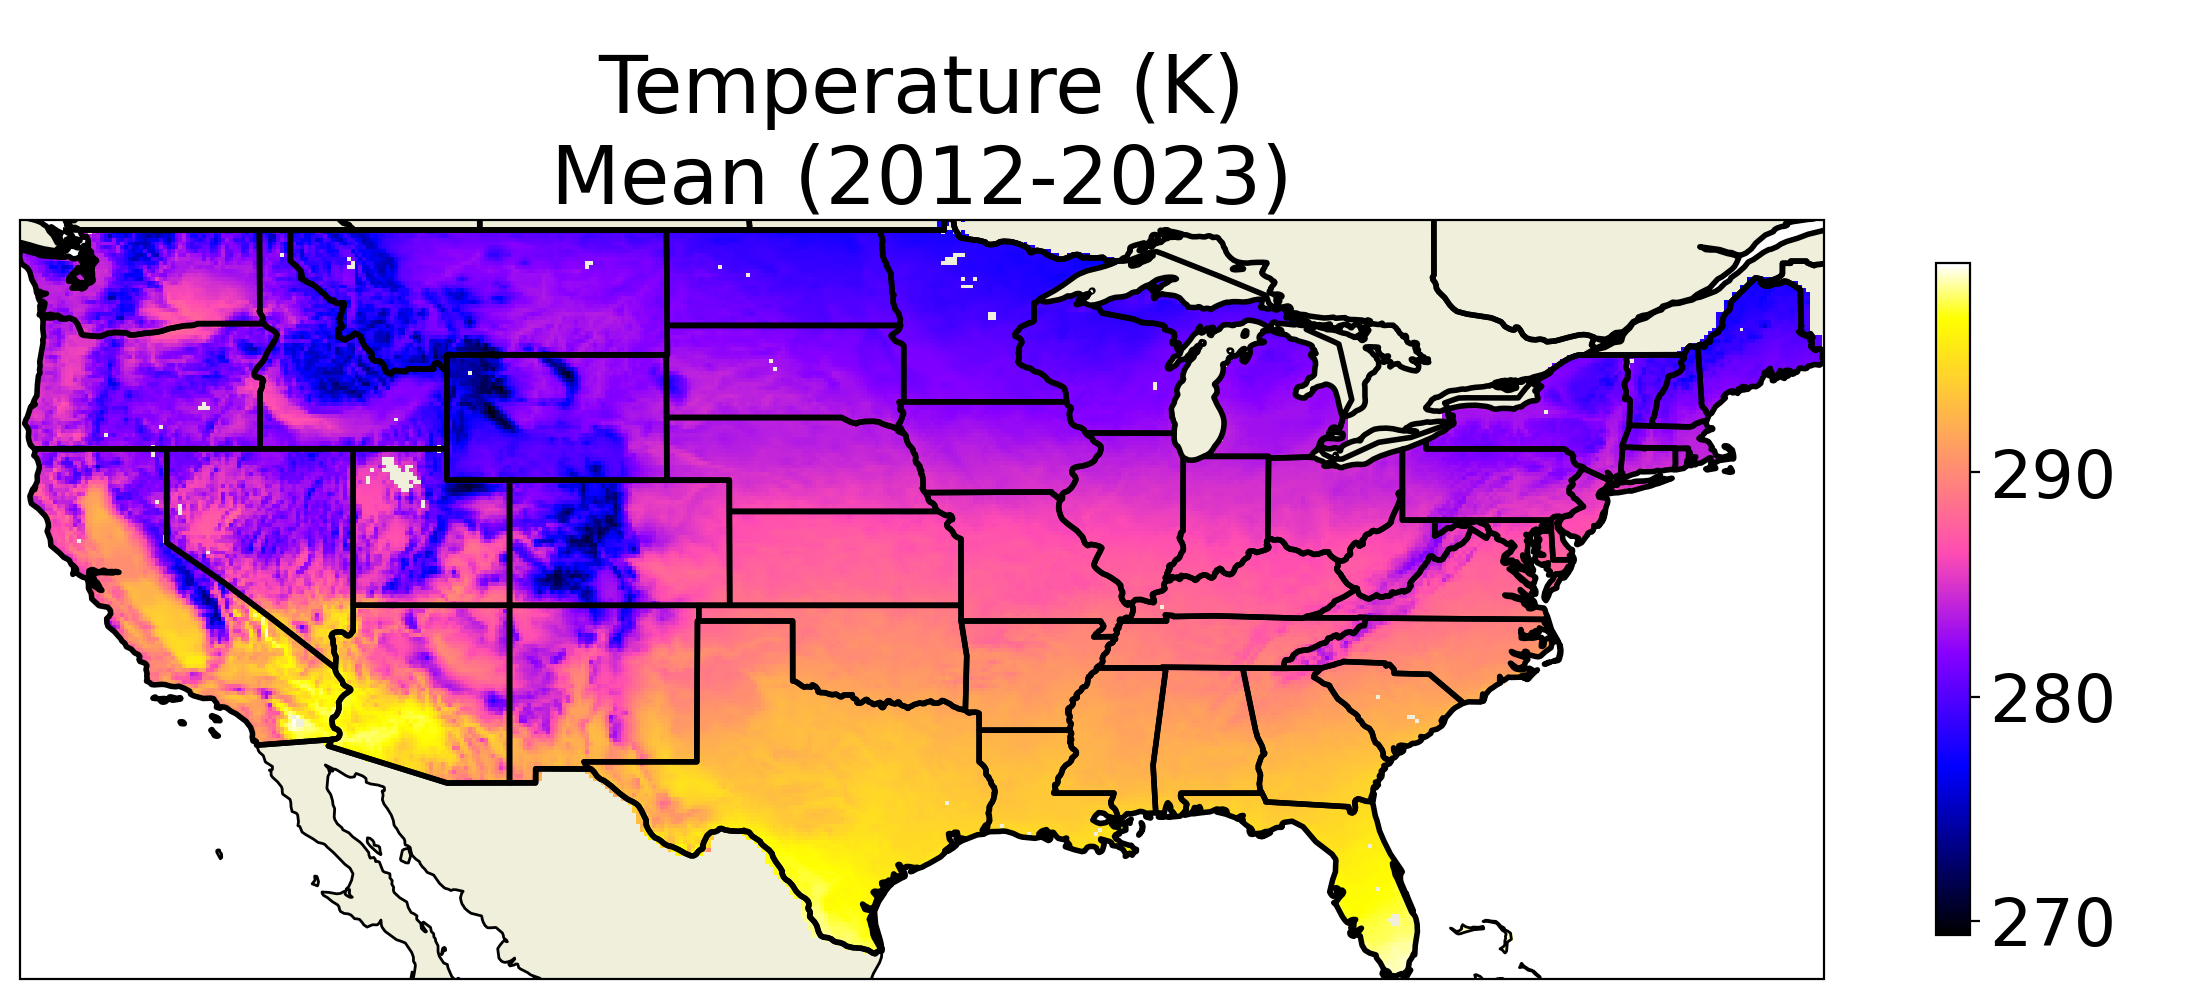
\includegraphics[width=.48\linewidth]{figures/thesis-gridstats/gridstat-bulk_tmp_2012-1_2023-12_y000-195_x000-462_mean.png}
    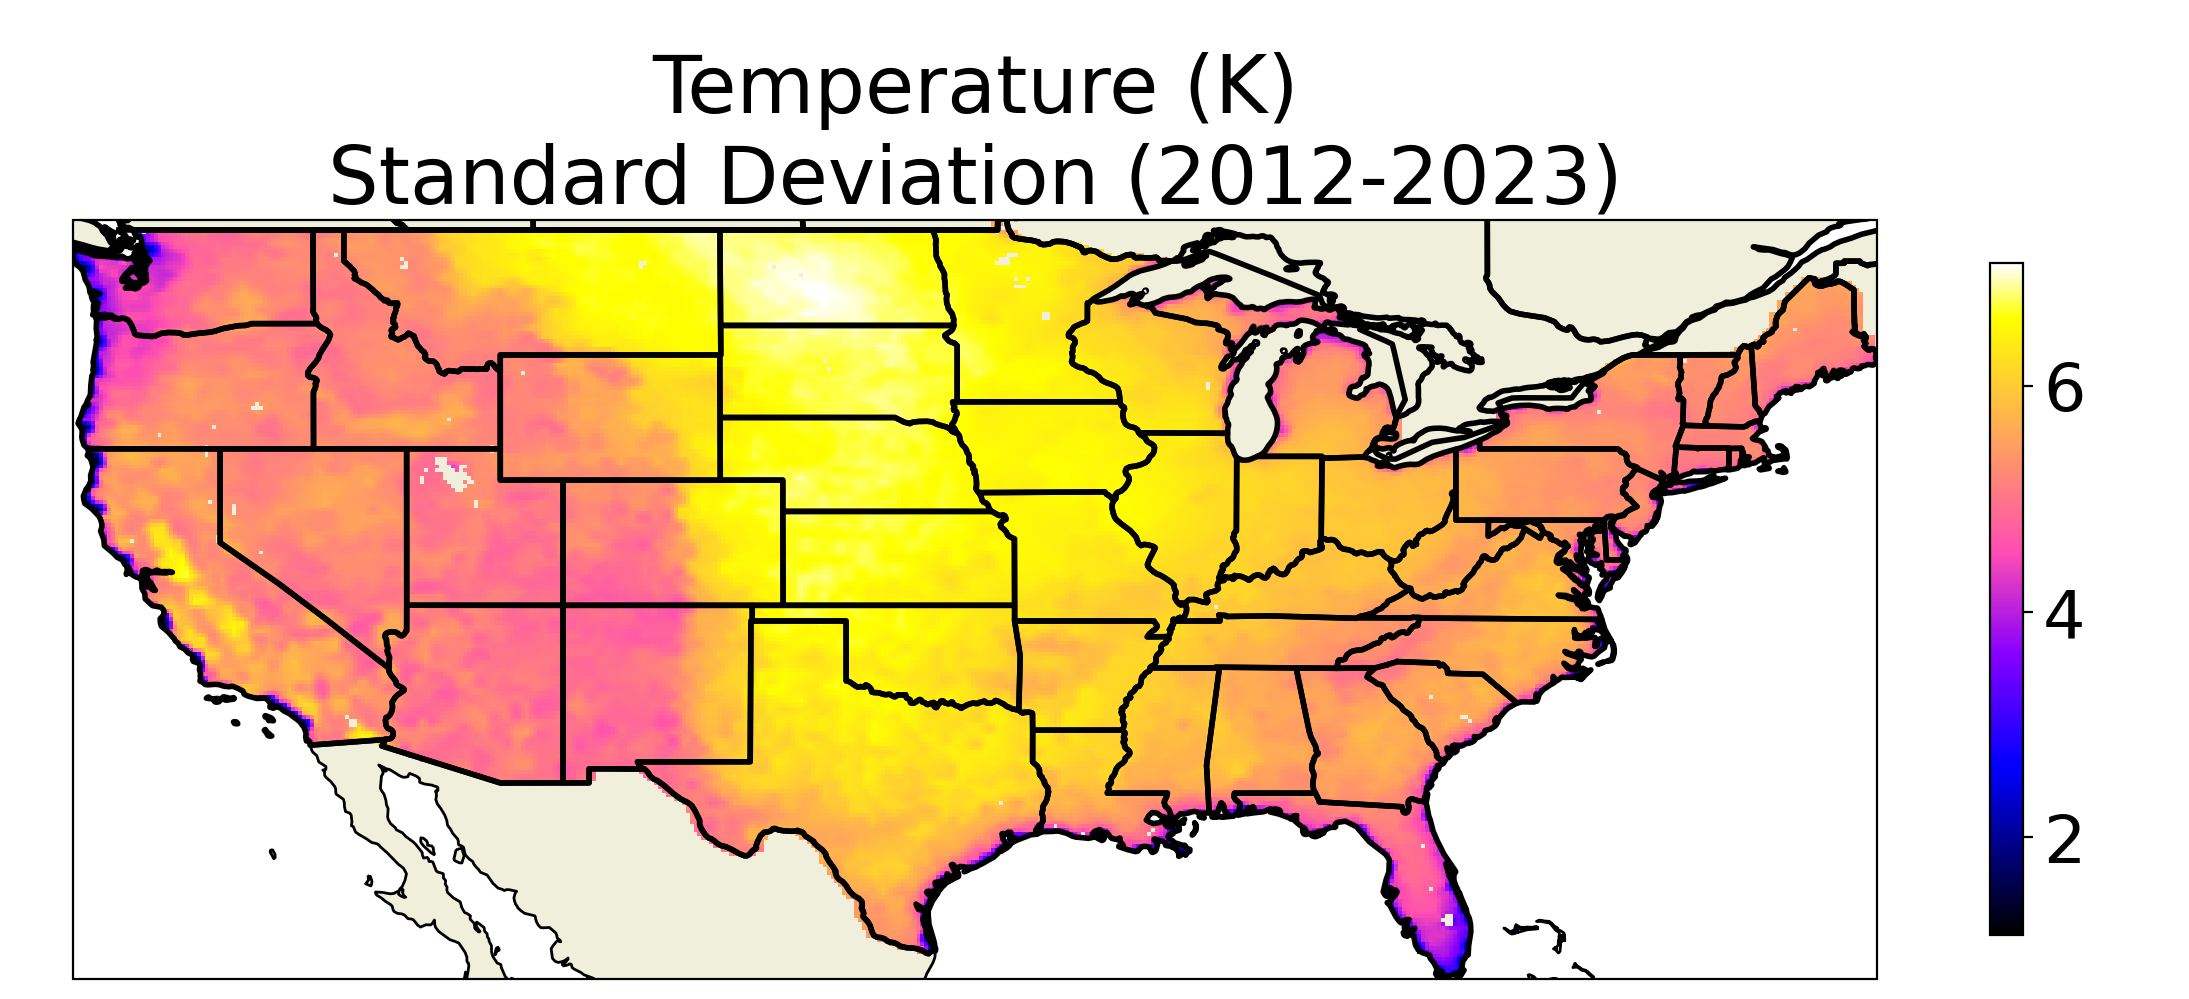
\includegraphics[width=.48\linewidth]{figures/thesis-gridstats/gridstat-bulk_tmp_2012-1_2023-12_y000-195_x000-462_stdev.png}

    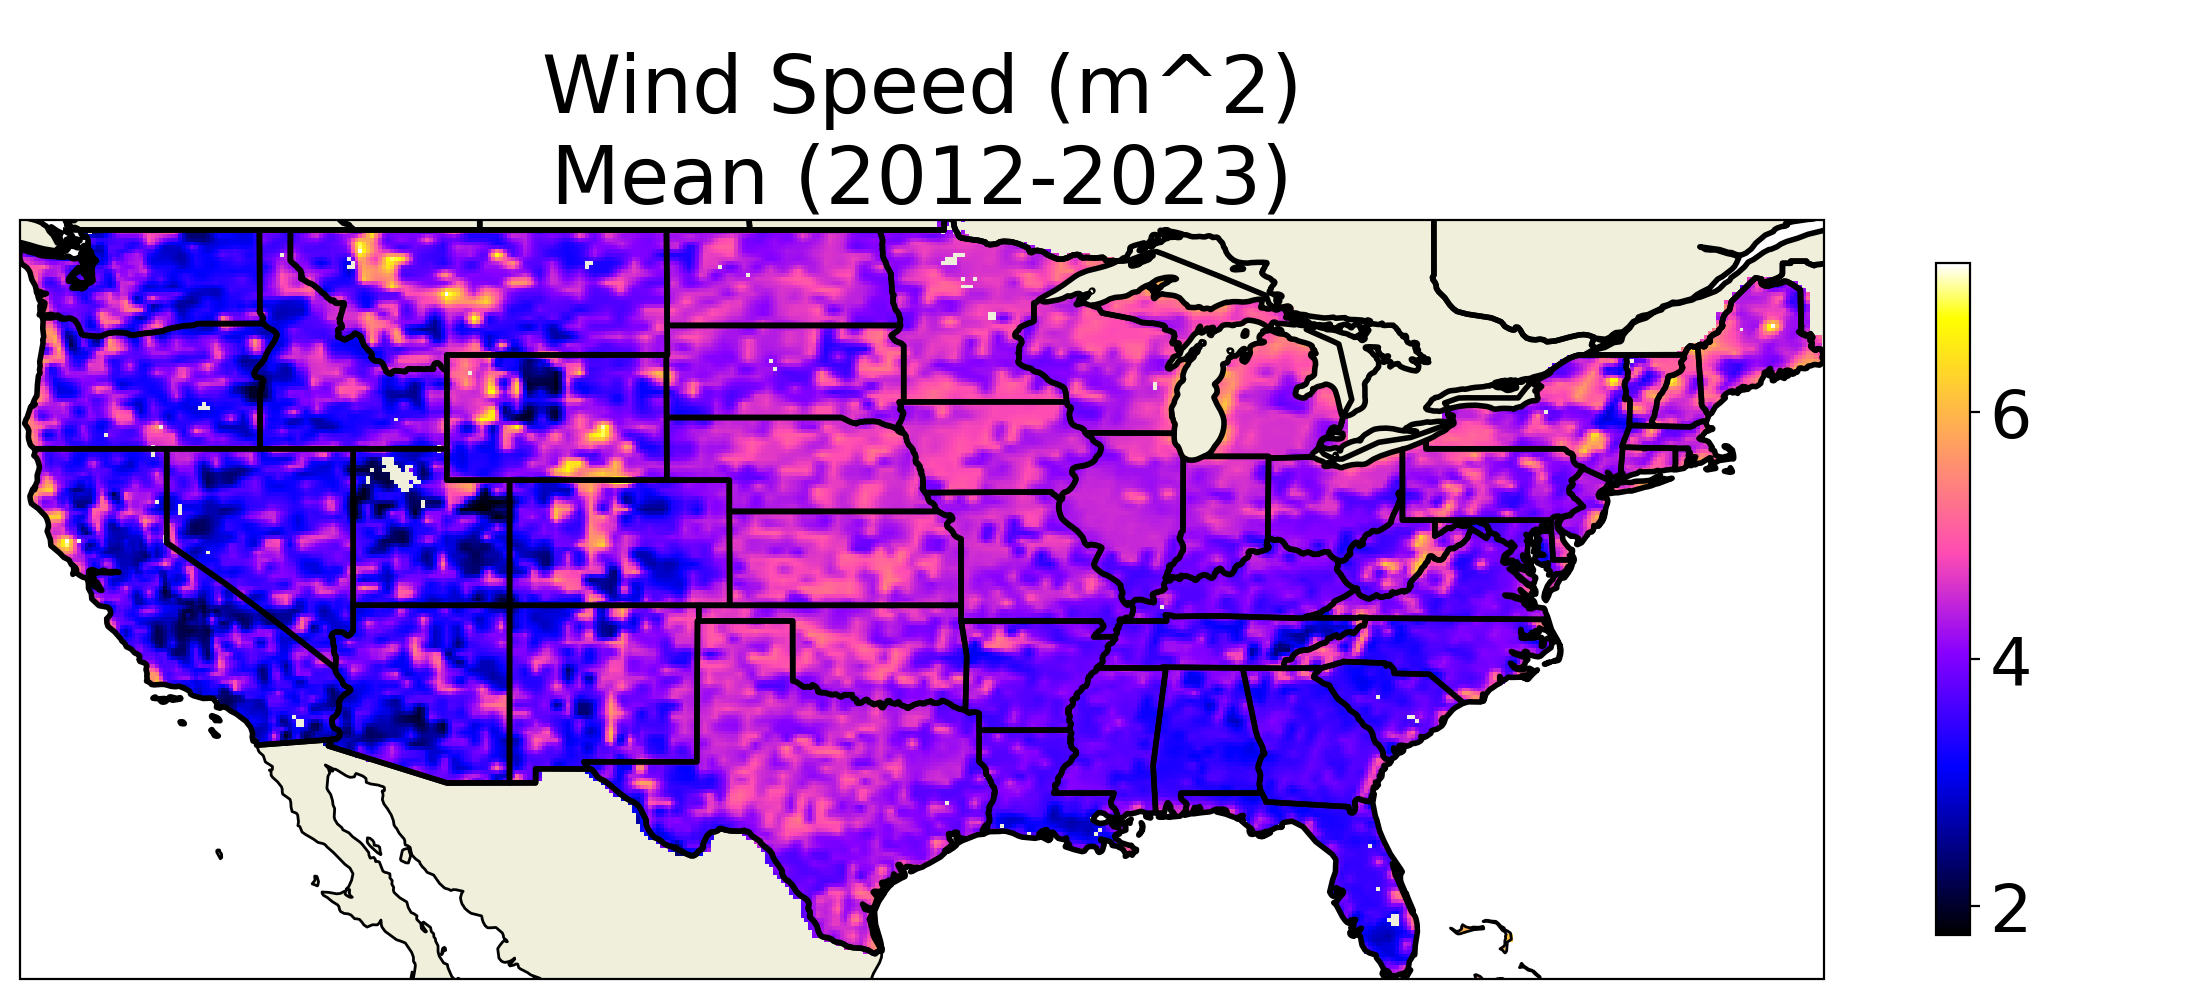
\includegraphics[width=.48\linewidth]{figures/thesis-gridstats/gridstat-bulk_windmag_2012-1_2023-12_y000-195_x000-462_mean.png}
    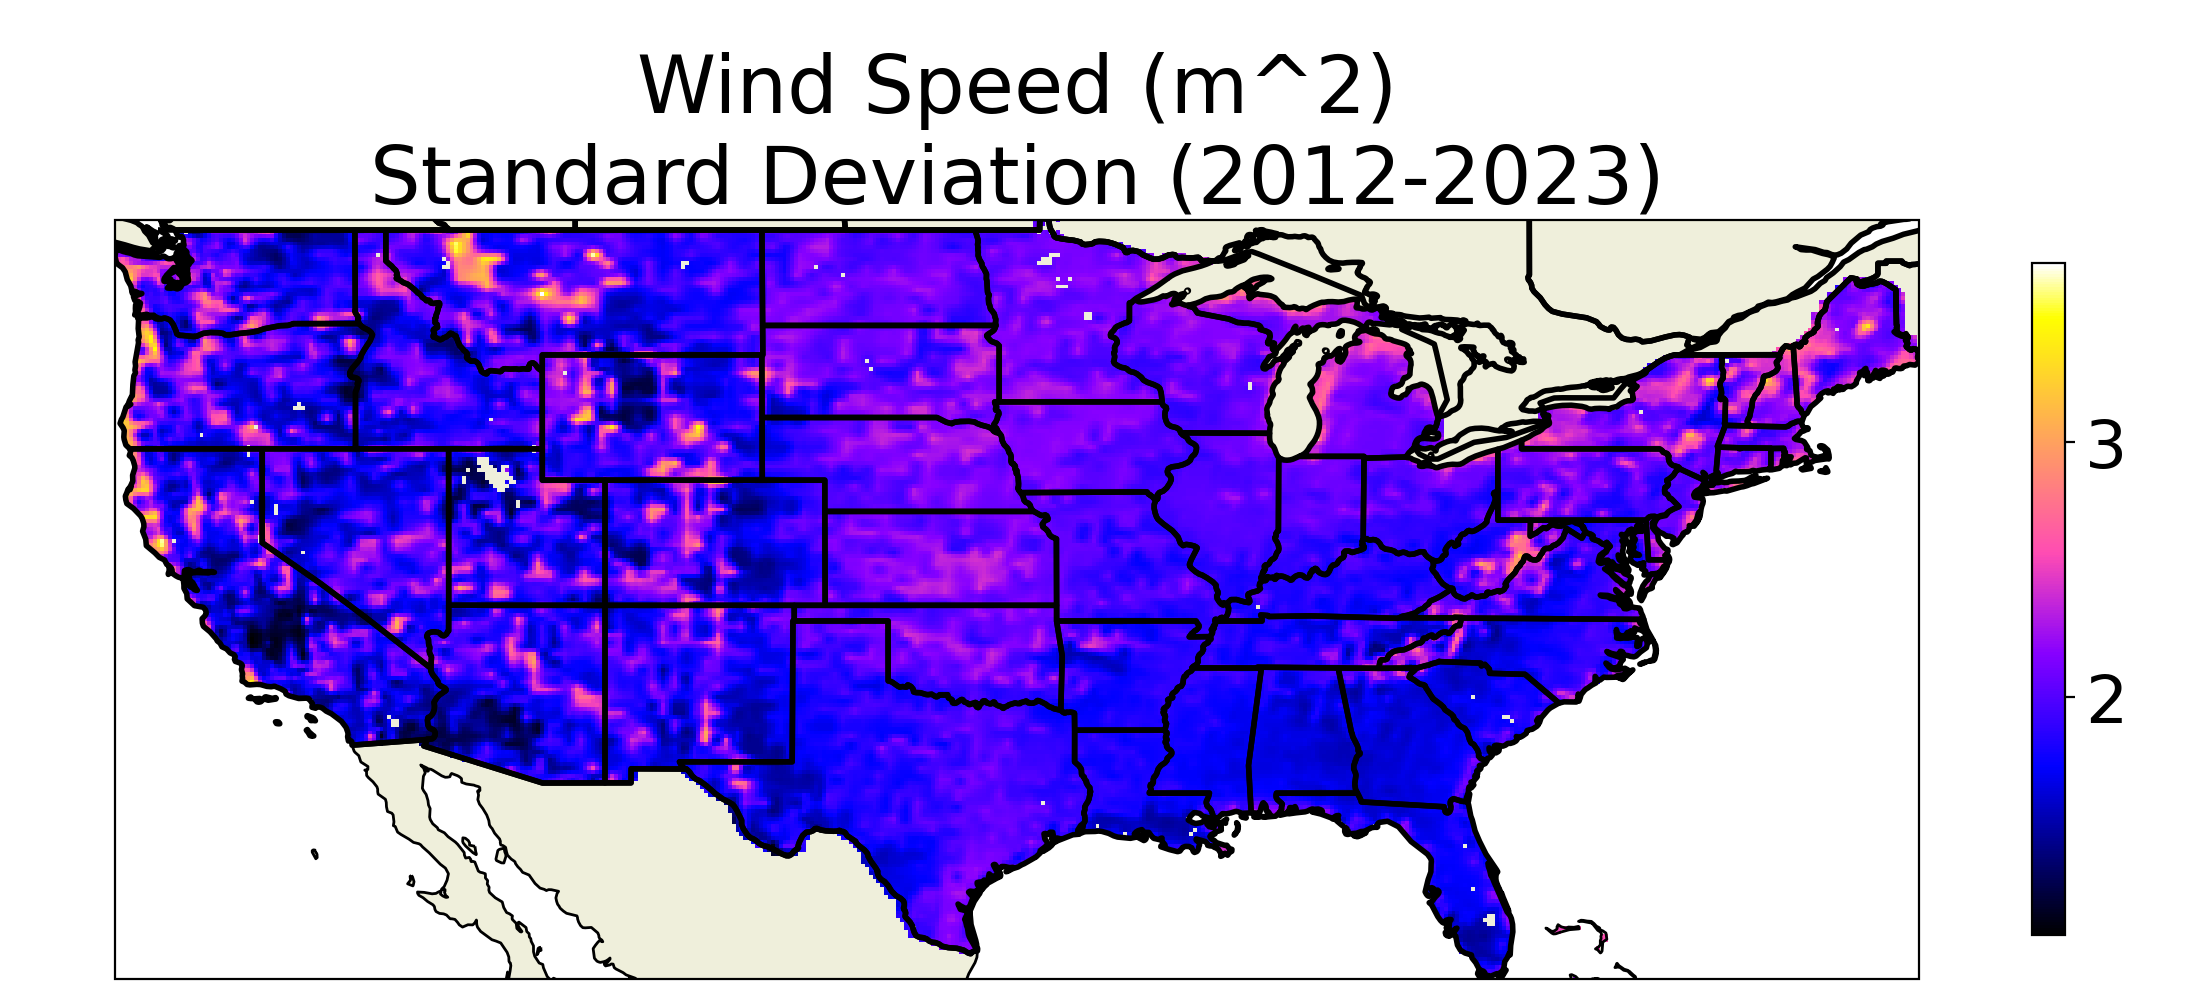
\includegraphics[width=.48\linewidth]{figures/thesis-gridstats/gridstat-bulk_windmag_2012-1_2023-12_y000-195_x000-462_stdev.png}
    \caption{Gridded mean and standard deviation of input forcings (2012-2023).}
    \label{gs-forcings}
\end{figure}

Figure \ref{gs-forcings} displays the same statistics for each of the other input forcings. The precipitation dataset includes liquid rain and snow, and reflects that the highest average values fell in the Pacific Coastal, Cascade, and Sierra Nevada, followed by more moderate values in the broad expanse of the Southeast, with the deep south of Louisiana and Mississippi seeing the strongest variability in precipitation throughout the year. Pressure mainly correlates with altitude, and higher latitudes tend to see the most variance, likely due to the prolonged influence of Rossby waves. Humidity and temperature also strongly correlate with temperature and proximity to the warm gulf, where the highest humidity variance is in the southern states thanks to seasonal intrusions of warm, moist air. The highest temperature variance is found in the high plains where there are considerable intrusions of arctic air in the winter, and solar heating combined with warm air advection from the terrain-driven low level jet in the summer. The wind is locally strongest where there is channeling from mountain slopes, with a broad region of relatively high wind speeds in the plains due to the open terrain.

\subsection{Handling Snow}

\begin{figure}[hb!]
    \centering
    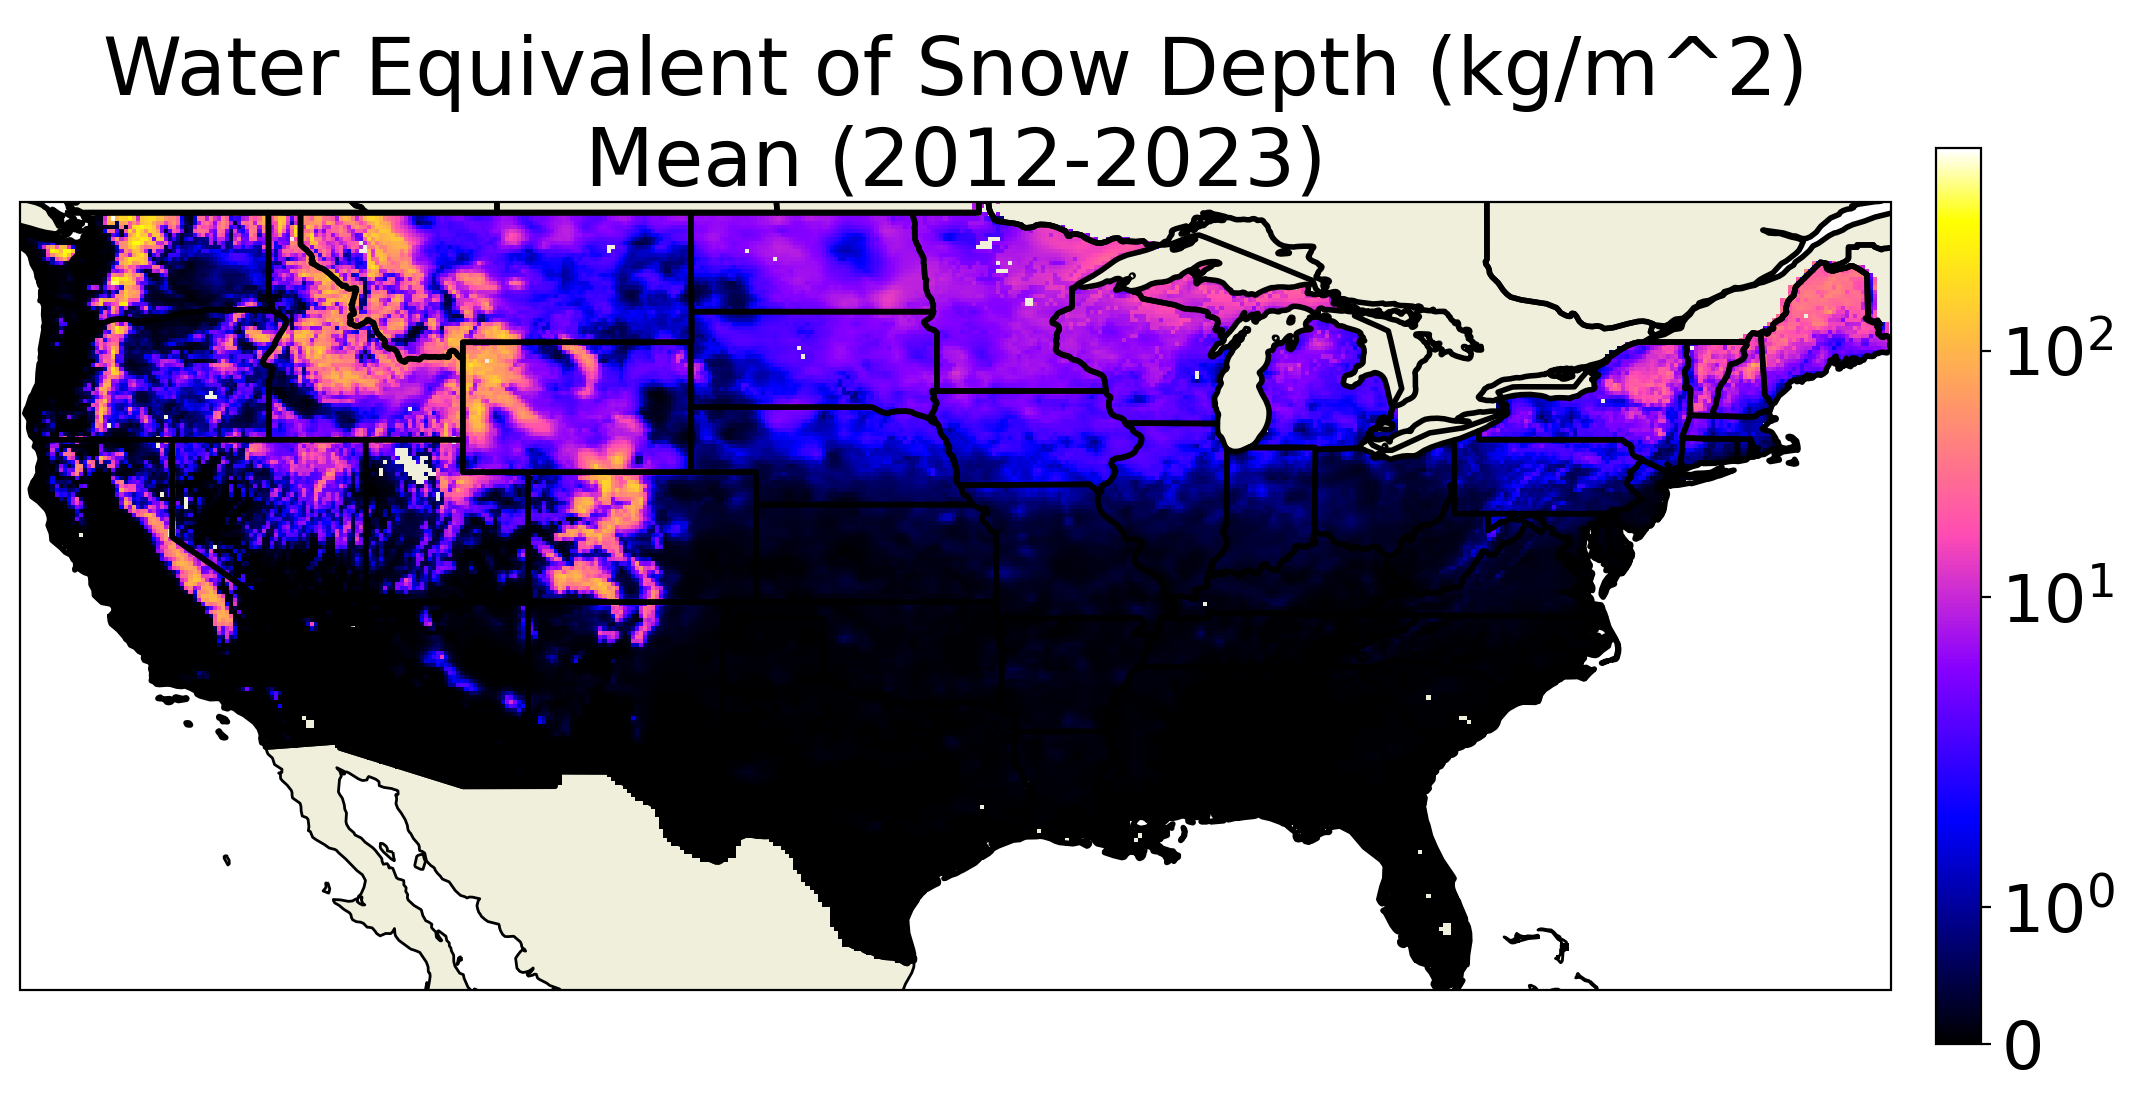
\includegraphics[width=.48\linewidth]{figures/thesis-gridstats/gridstat-bulk_weasd-log_2012-1_2023-12_y000-195_x000-462_mean.png}
    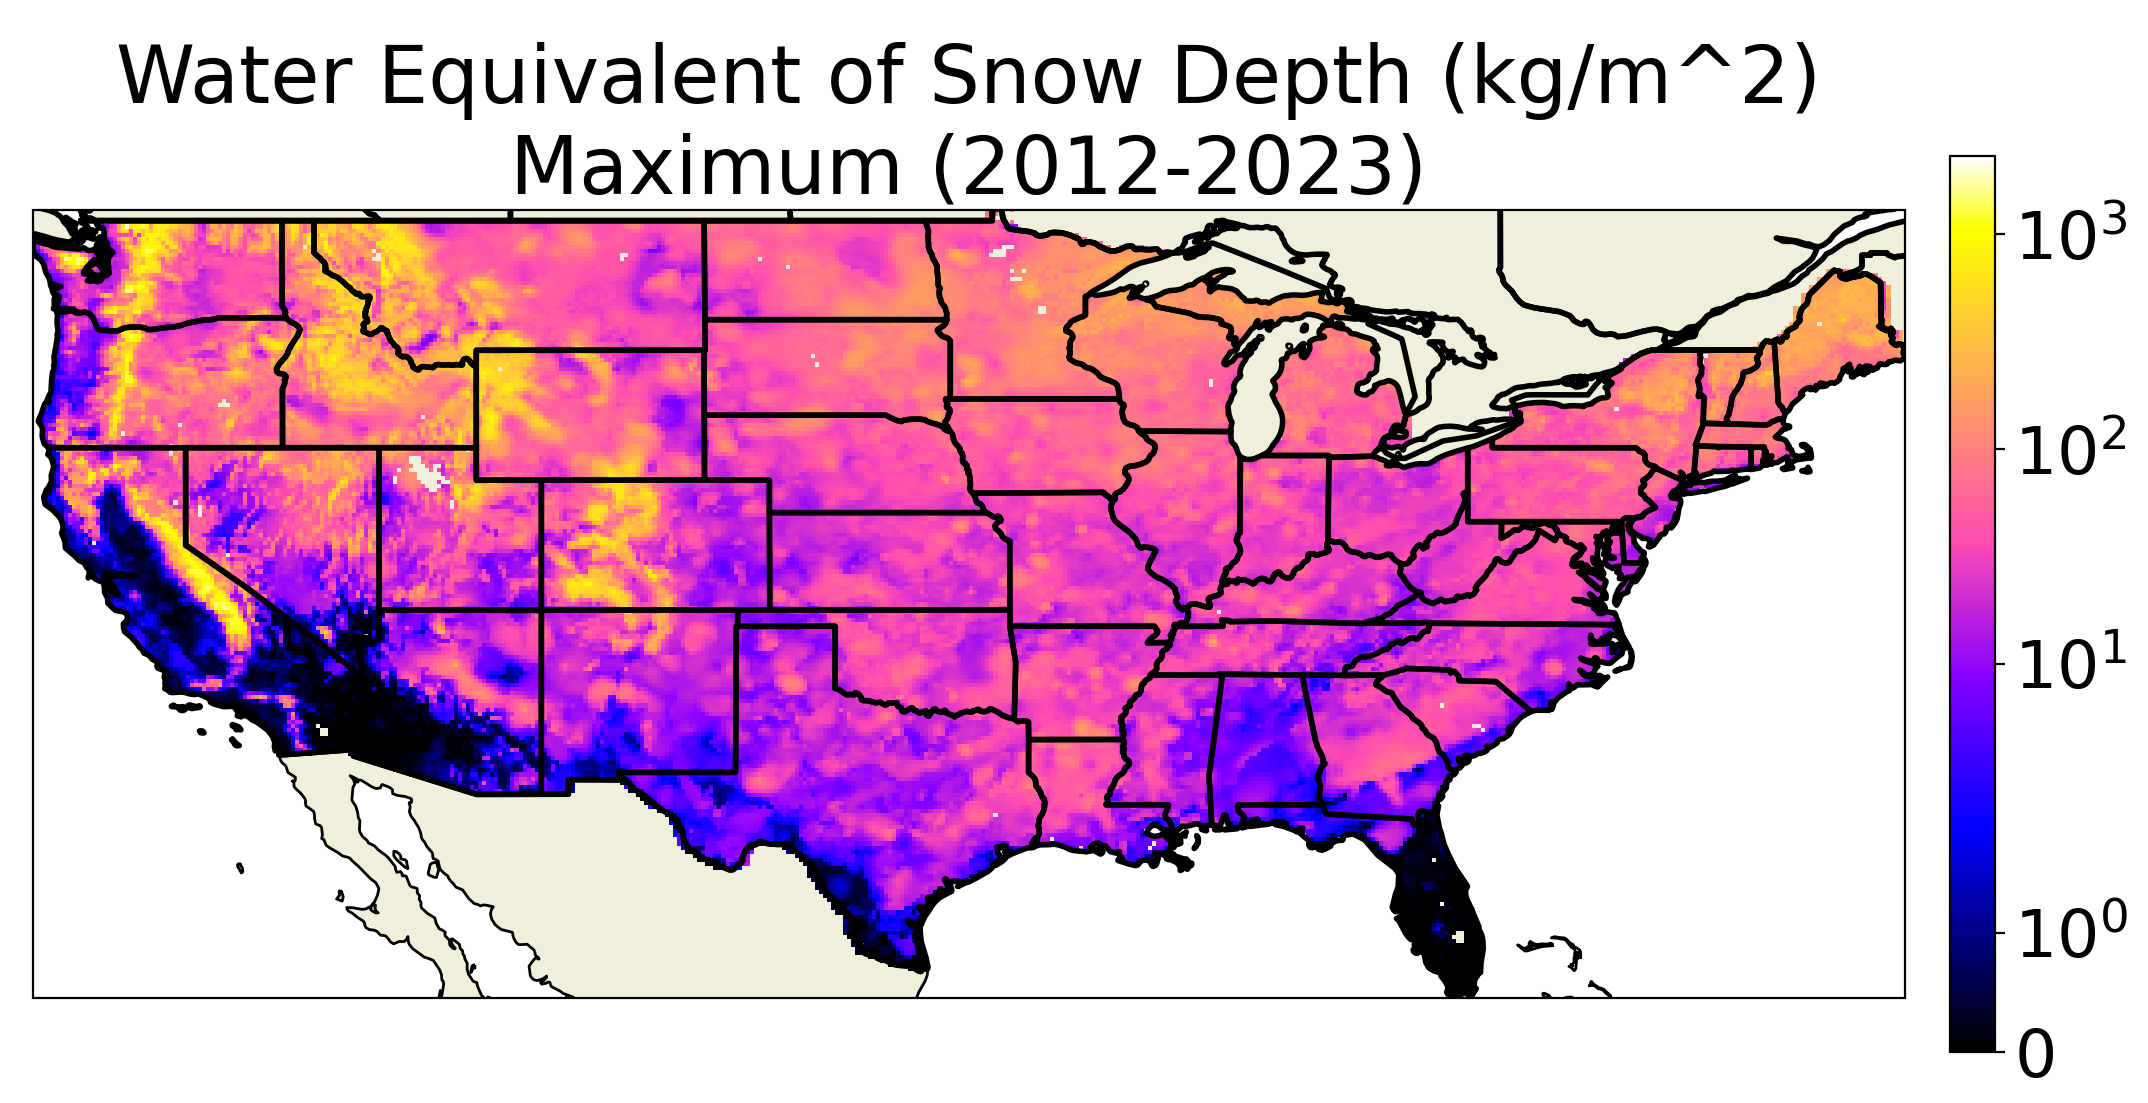
\includegraphics[width=.48\linewidth]{figures/thesis-gridstats/gridstat-bulk_weasd-log_2012-1_2023-12_y000-195_x000-462_max.png}
    \caption{Mean and maximum accumulated snow amounts on a log scale (2012-2023).}
    \label{gs-snow}
\end{figure}

Figure \ref{gs-snow} shows the mean and maximum snow accumulation throughout the dataset. Snow is particularly difficult to account for in the ANNs because it is relatively rare and highly regional, but has a profound influence on the soil dynamics. The presence of snow significantly modifies the surface albedo and roughness length, captures and stores precipitation as an additional state variable, and represents a new source of water for the soil column as it melts \parencite{koren_parameterization_1999}. The first exploratory models we trained treated snow as essentially an additional soil layer, and predicted the increment change in its value alongside the other soil states. Since snow is such a transient phenonmenon within the training dataset the ANNs would consistently predict close to zero change, even in snowy conditions, since doing so results in the lowest loss in most cases.

\begin{figure}[hb!]
    \centering
    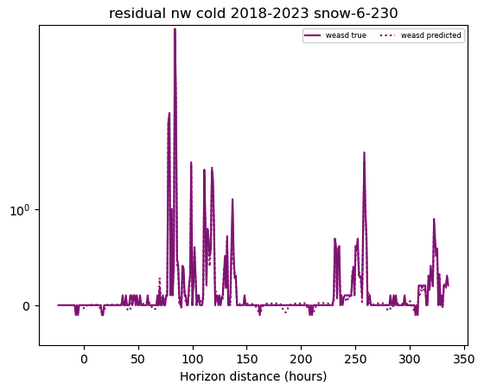
\includegraphics[width=.32\linewidth]{figures/snow-sample_res.png}
    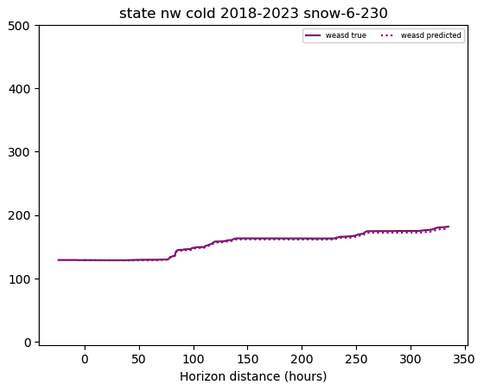
\includegraphics[width=.32\linewidth]{figures/snow-sample_state.png}
    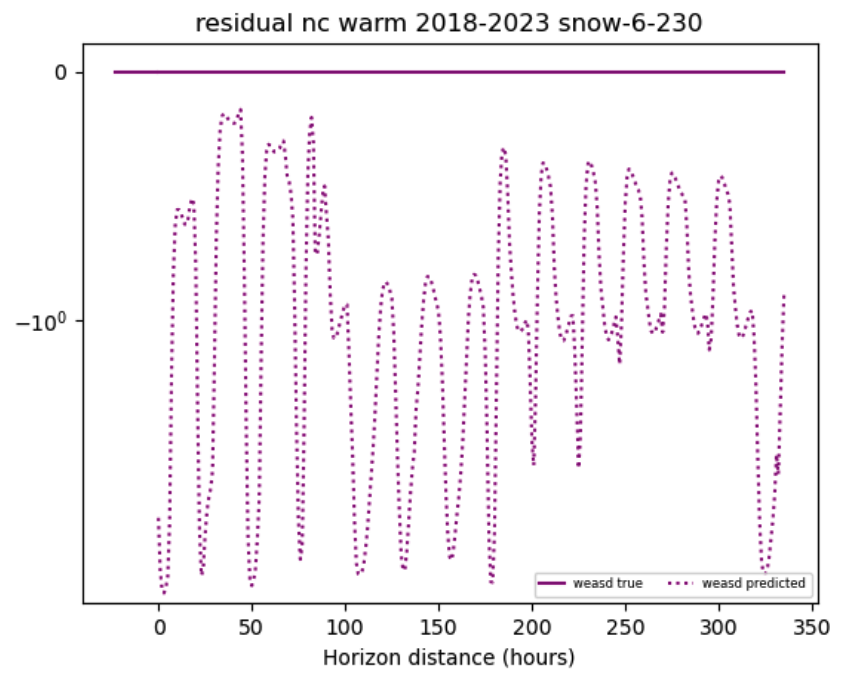
\includegraphics[width=.32\linewidth]{figures/snow-sample_warm.png}
    \caption{Samples of snow-only model predictions vs true values after loss function manipulation, including the increment change for a significant snowfall event (left), the accumulated state for the same sample (center), and an example of the increment outputs of a different warm-season sample (right).}
    \label{snow-models}
\end{figure}

Subsequent models trained to exclusively target the increment change in snow water equivalent showed the same hesitancy to make non-zero predictions. In order to loosen the requirement that these models must always output zero change when there is no snow present, we modified the loss function used to train the snow-only models such that predicting negative increment change values when there is no snow present will not be penalized. When combined with a post-processing step that truncates negative accumulated snow amounts at zero, this strategy focuses the gradient descent process exclusively on samples where the snow pack is relevant.

Figure \ref{snow-models} displays a sample from one of these loss-modified snow models, which captures the subtleties of extreme snow events, and maintains negative increment predictions when there is no snow present or accumulating. Curiously, the negative predictions of the model during the warm-season sample cycle on a diurnal basis, and may represent a hypothetical snow melt rate, which is an emergent property since the loss function was not applied in such scenarios. In any case, although these are encouraging preliminary results, further refinement of this strategy is out of the scope of this project. We will use the true snow amount as an input to the soil moisture ANNs presented here in order to prevent compounding error, and take the apparent validity of this approach as an indication that separate ANNs designed specifically for snow water equivalent estimation may be used to initialize soil moisture emulators in the future.

\subsection{Input Data Value Distributions}

\begin{figure}[hb!]
    \centering
    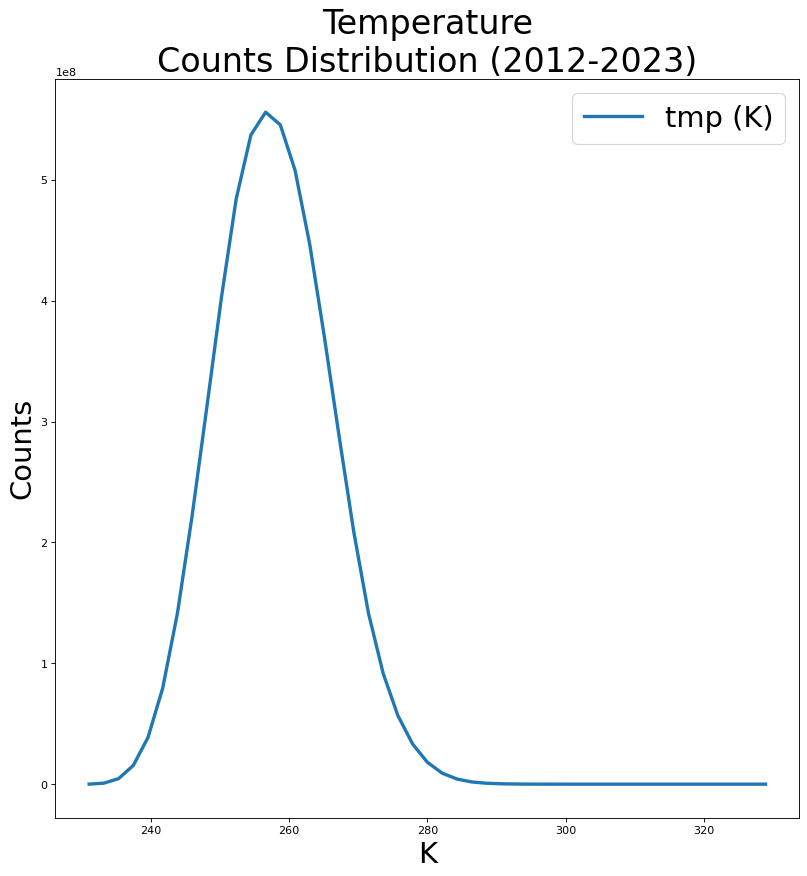
\includegraphics[width=.24\linewidth]{figures/thesis-gridstats/gridstat-hist_tmp_2012-1_2023-12_y000-195_x000-462.png}
    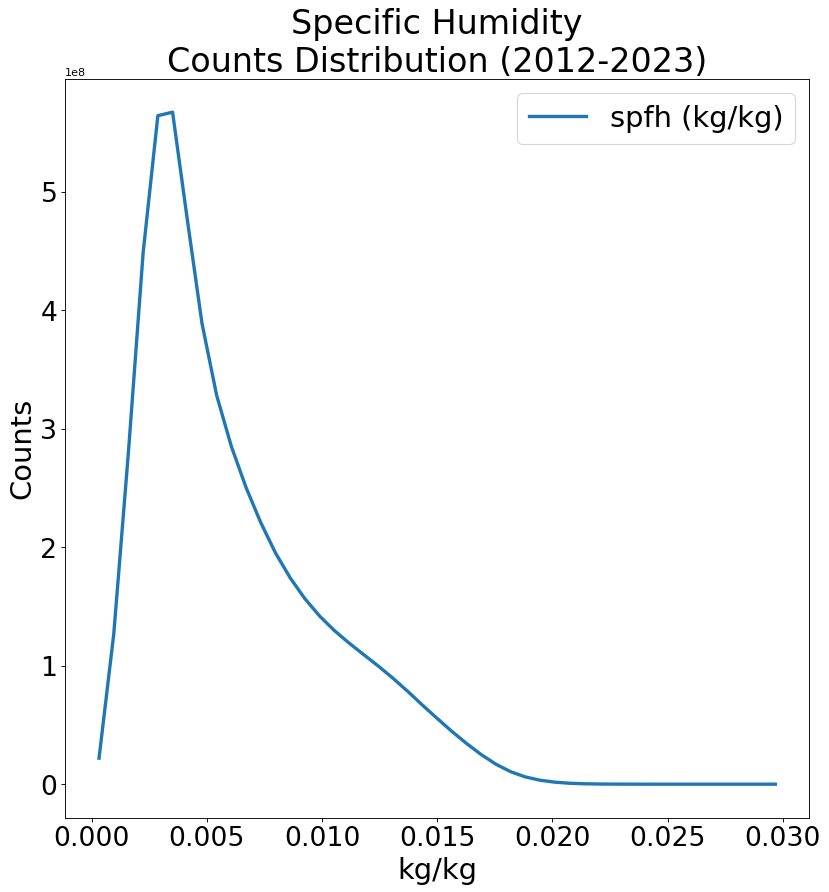
\includegraphics[width=.24\linewidth]{figures/thesis-gridstats/gridstat-hist_spfh_2012-1_2023-12_y000-195_x000-462.png}
    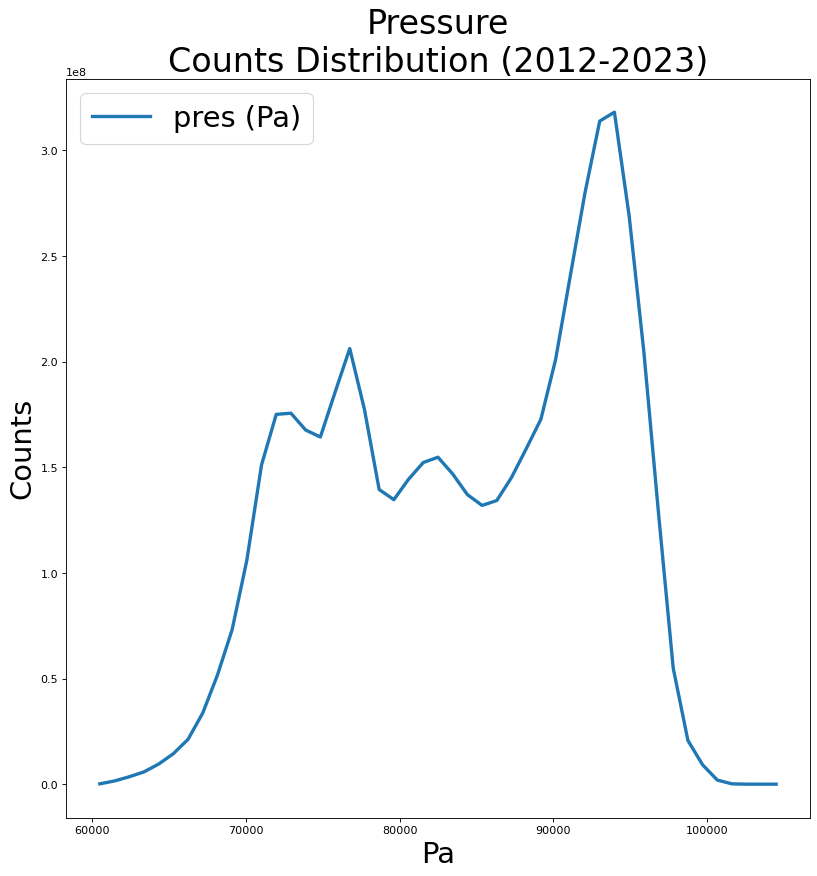
\includegraphics[width=.24\linewidth]{figures/thesis-gridstats/gridstat-hist_pres_2012-1_2023-12_y000-195_x000-462.png}
    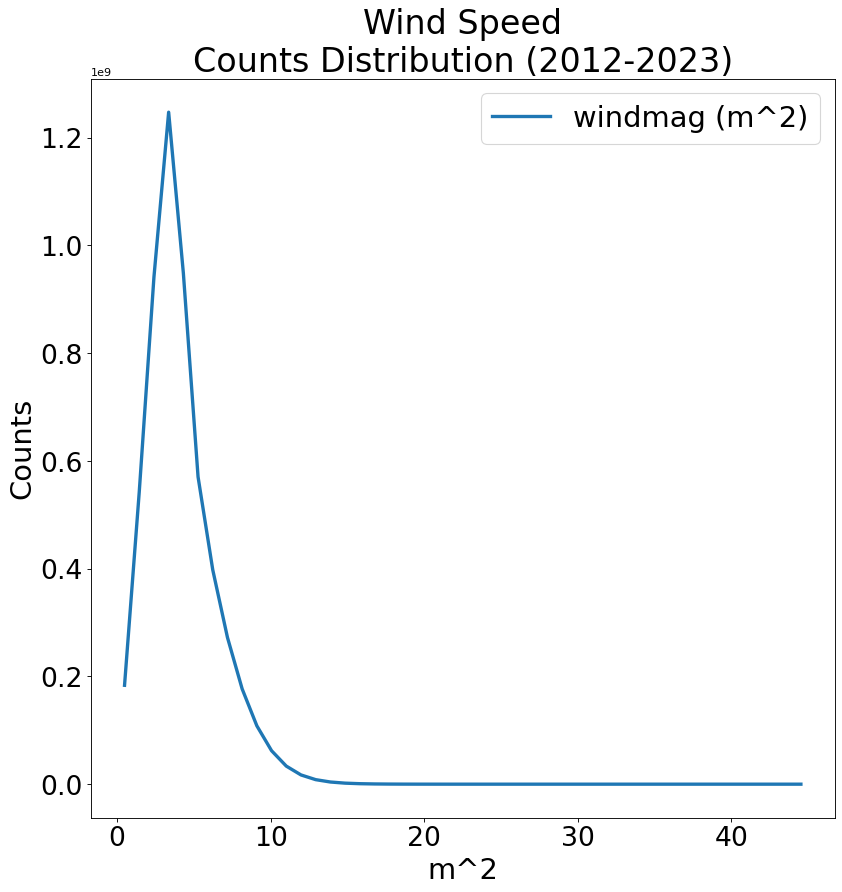
\includegraphics[width=.24\linewidth]{figures/thesis-gridstats/gridstat-hist_windmag_2012-1_2023-12_y000-195_x000-462.png}

    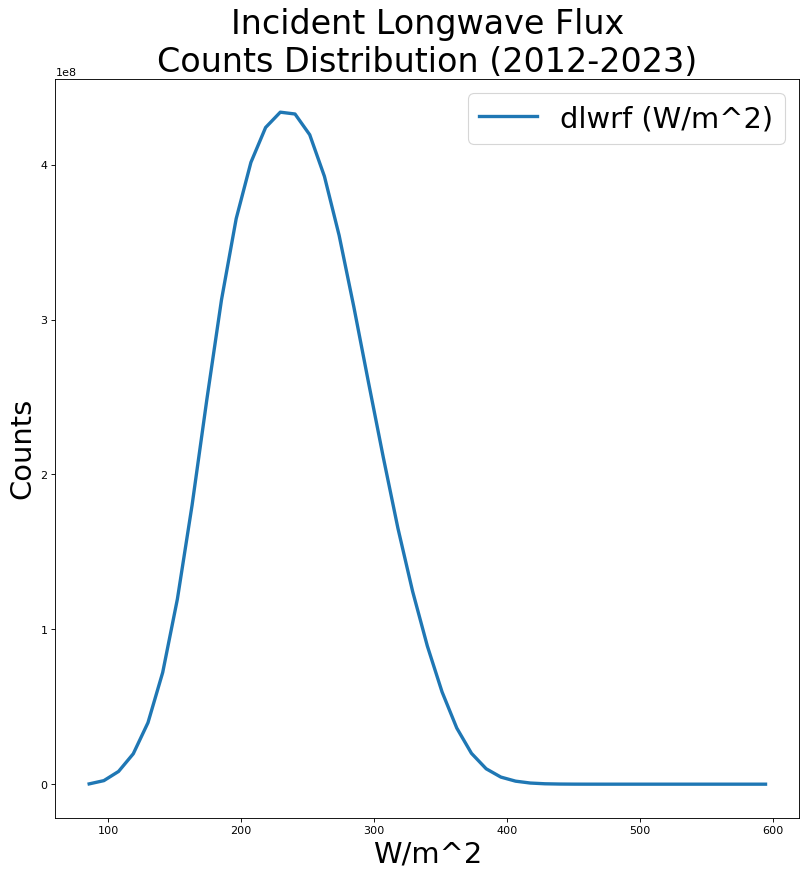
\includegraphics[width=.24\linewidth]{figures/thesis-gridstats/gridstat-hist_dlwrf_2012-1_2023-12_y000-195_x000-462.png}
    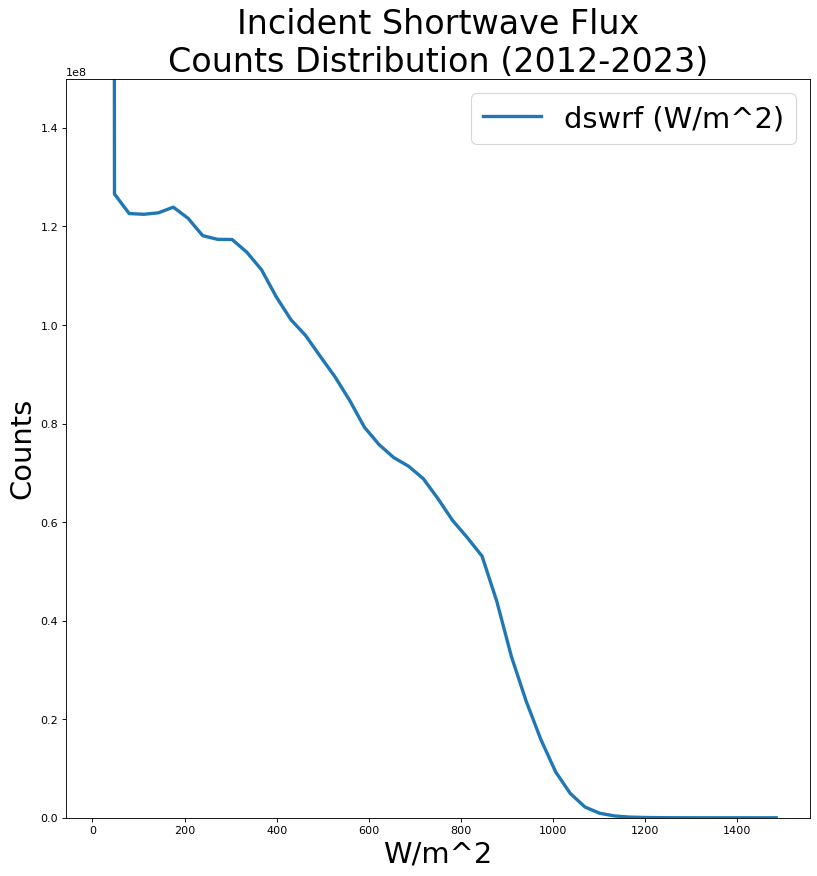
\includegraphics[width=.24\linewidth]{figures/thesis-gridstats/gridstat-hist_dswrf_2012-1_2023-12_y000-195_x000-462.png}
    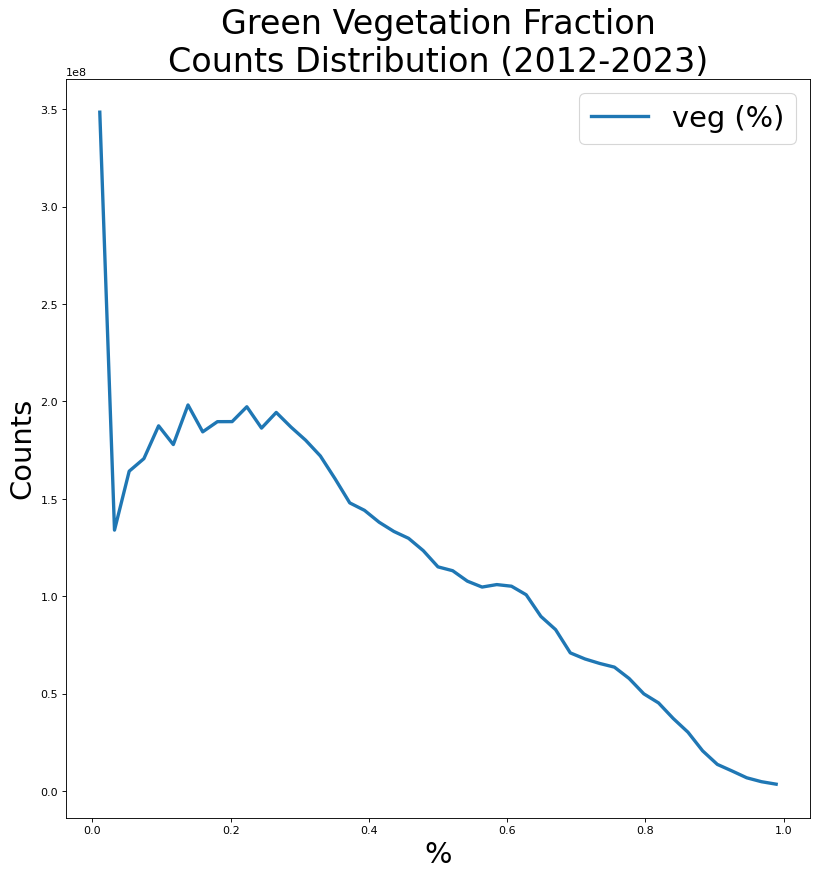
\includegraphics[width=.24\linewidth]{figures/thesis-gridstats/gridstat-hist_veg_2012-1_2023-12_y000-195_x000-462.png}
    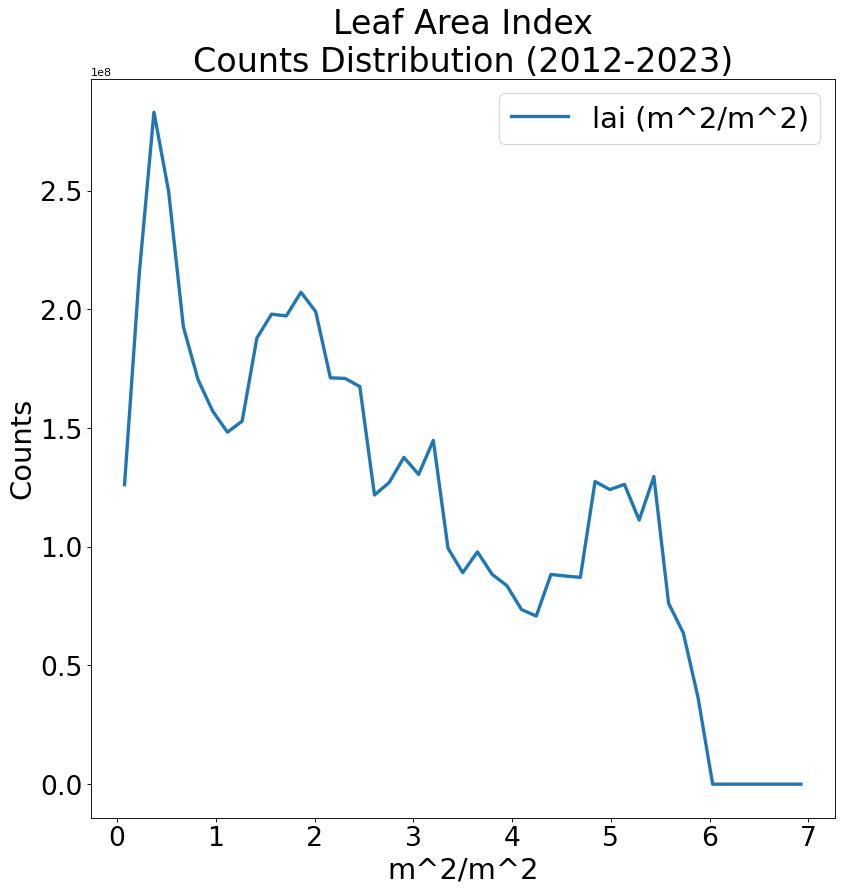
\includegraphics[width=.24\linewidth]{figures/thesis-gridstats/gridstat-hist_lai_2012-1_2023-12_y000-195_x000-462.png}

    \caption{Overall distributions of dynamic model inputs (2012-2023).}
    \label{dist-forcings}
\end{figure}

The count distributions of dynamic inputs with the exception of precipitation are displayed by Figure \ref{dist-forcings}. Of these only temperature and incident longwave flux follow generally gaussian distributions. Specific humidity is strongly skewed toward zero since its upper bound is limited by temperature. Pressure has a global peak just below sea level pressure, with relative maxima associated with the mountainous terrain of Appalachia and the West. Windspeed has a strong peak around 5 $m s^{-1}$, with a long tail of outliers. Shortwave flux is not entirely smooth, which is likely due in part to enhanced cloud cover from orographic effects, judging by the spatial distribution in Figure \ref{gs-radiative}. The vegetation parameters are also strongly non-gaussian owing to their regional and seasonal heterogeneity, and the discrete differences in vegetation categories.


\begin{figure}[h!]
    \centering
    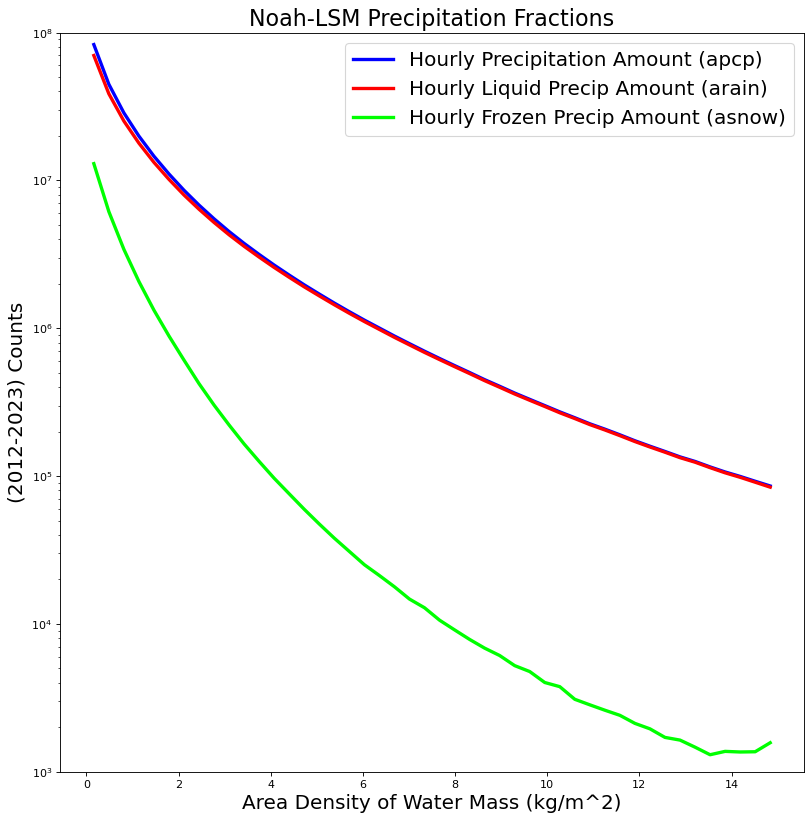
\includegraphics[width=.48\linewidth]{figures/thesis-gridstats/gridstat-hist_groupings_preciptype.png}
    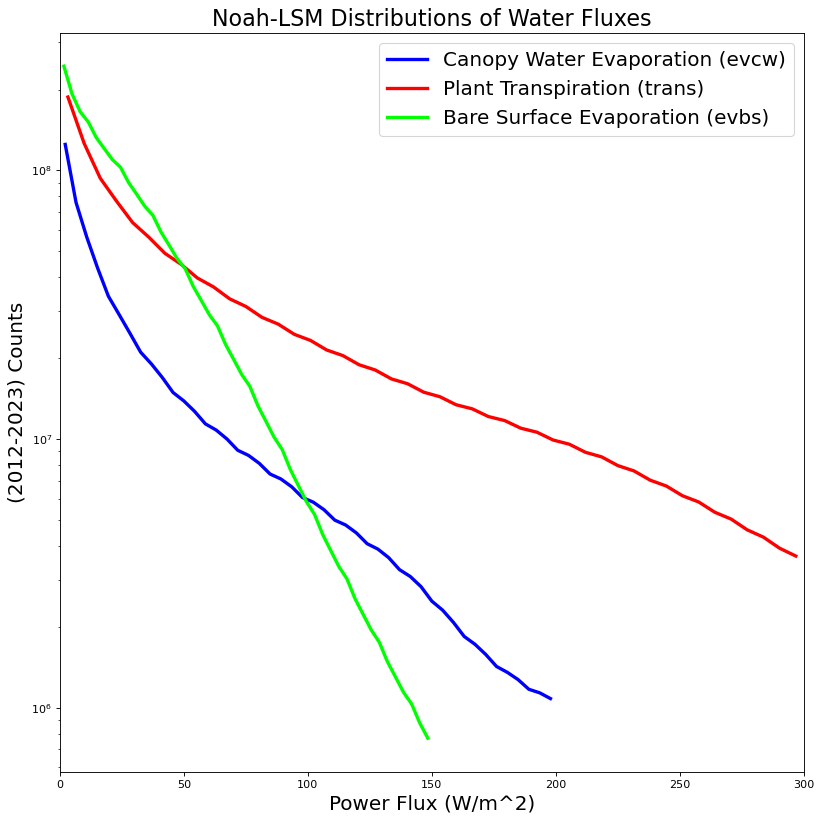
\includegraphics[width=.48\linewidth]{figures/thesis-gridstats/gridstat-hist_groupings_powerflux.png}
    \caption{Overall distributions of precipitation types (left) and fluxes removing water from the surface system (right), both on a logarithmic axis (2012-2023).}
    \label{dist-waterflux}
\end{figure}

Figure \ref{dist-waterflux} compares the distributions of precipitation types, and those of the fluxes that remove water from the system. Liquid precipitation represents the vast majority of the total hourly precipitation amount, especially for strong precipitation events. Plant transpiration is the dominant sink for soil moisture content, with bare surface evaporation mainly limited to lower rates. Evaporation from the plant canopy can also be relevant in mitigating the amount of water that percolated downward into the soil column after rain events. Each of the distributions extend further with higher-value outliers, however these were truncated during the statistic collection process in order to emphasize the shape of the more common lower-end values. Notice that all of these processes are plotted on a log axis in the figure for visual clarity, which belies the fact that these are extremely skewed distributions. Similar to snow as outlined in the previous subsection, although they are important processes within the model, the fluxes and precipitation -- and especially their upper extremes -- are ultimately rare in the context of the full dataset, which poses a challenge for statistical optimization techniques like deep learning.

\subsection{Soil Moisture Distribution and Metrics}

\begin{figure}[h!]
    \centering
    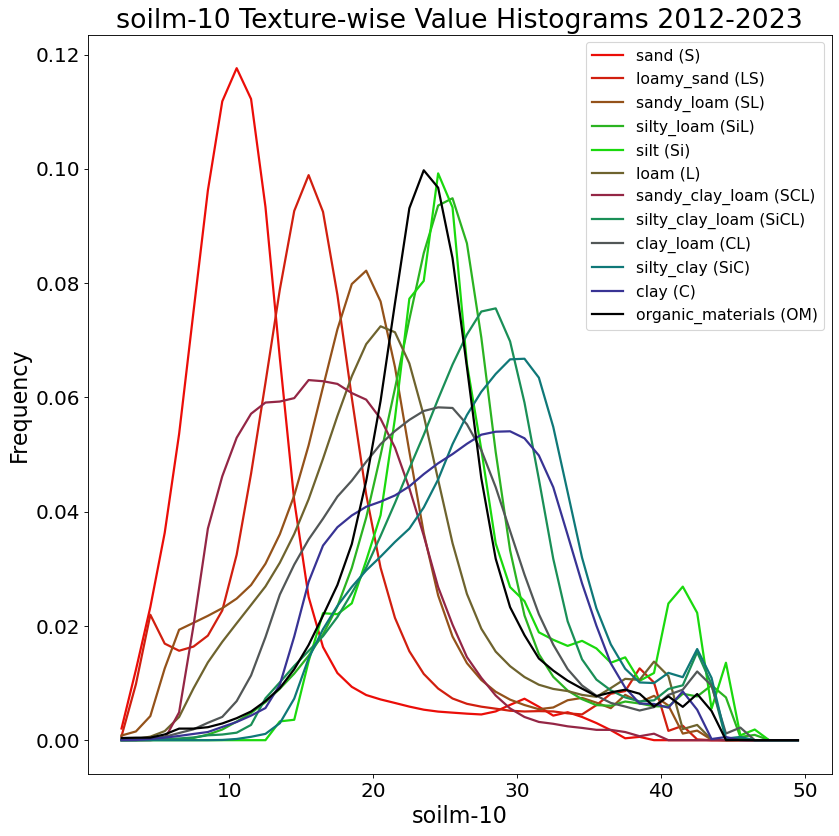
\includegraphics[width=.32\linewidth]{figures/thesis-gridstats/gridstat-hist-textures_soilm-10_2012-1_2023-12_y000-195_x000-462}
    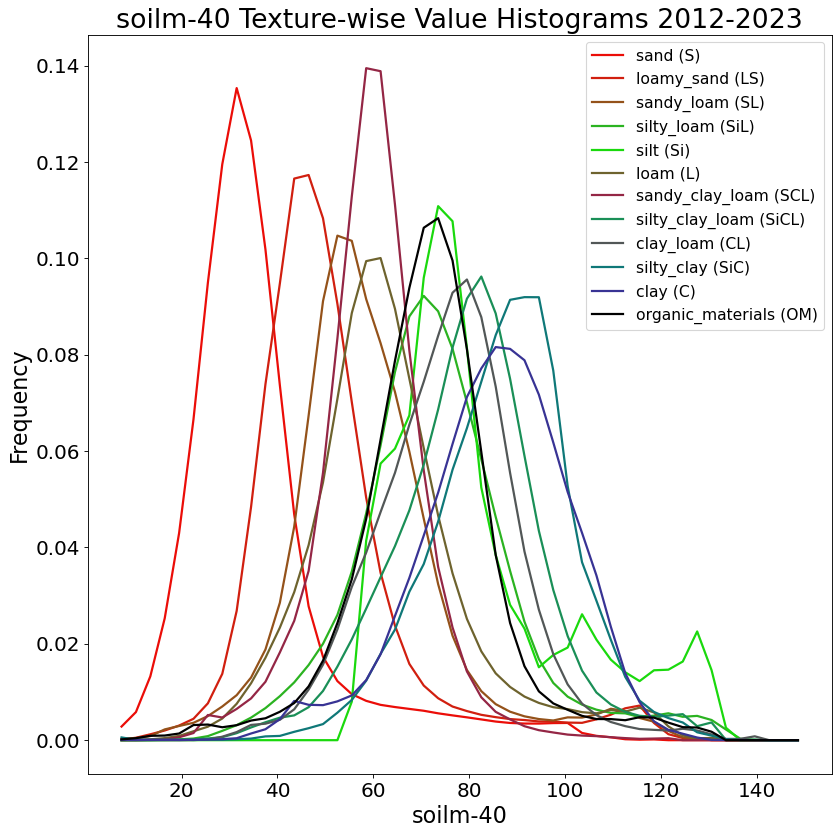
\includegraphics[width=.32\linewidth]{figures/thesis-gridstats/gridstat-hist-textures_soilm-40_2012-1_2023-12_y000-195_x000-462}
    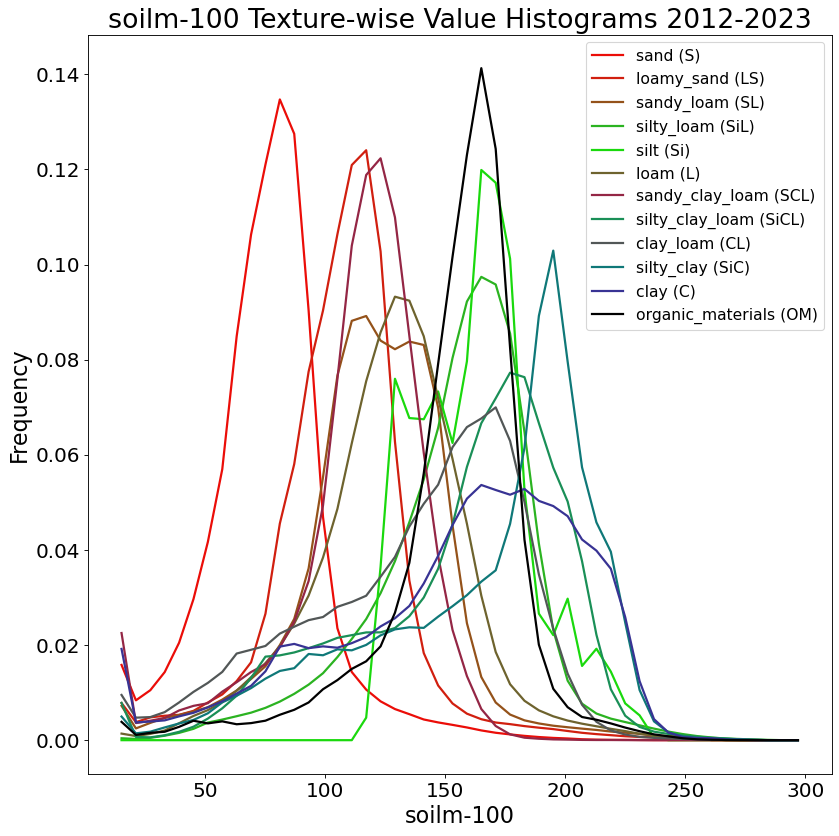
\includegraphics[width=.32\linewidth]{figures/thesis-gridstats/gridstat-hist-textures_soilm-100_2012-1_2023-12_y000-195_x000-462}

    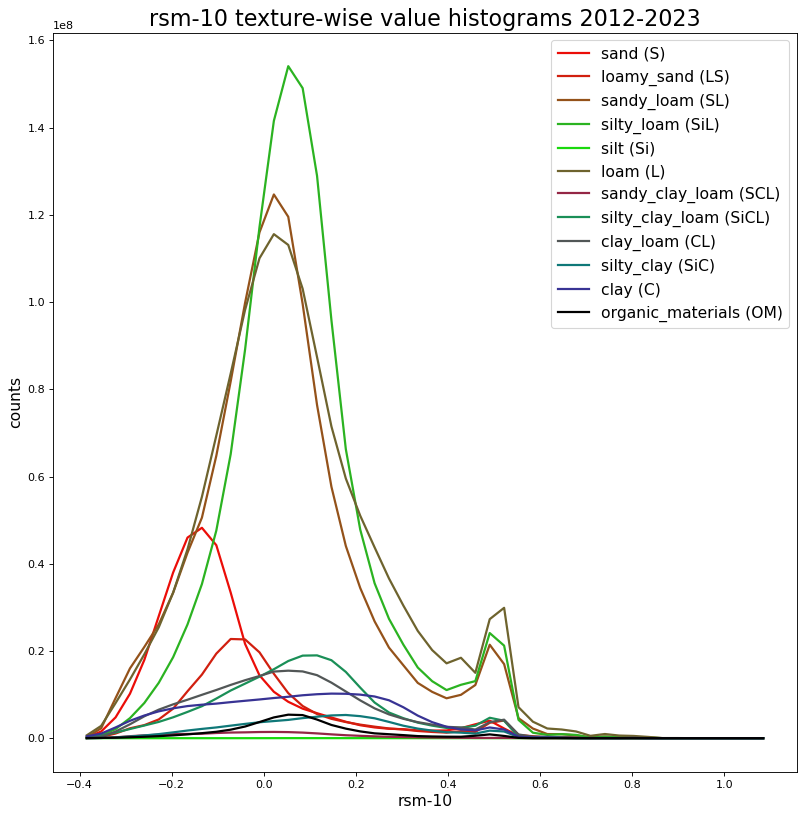
\includegraphics[width=.32\linewidth]{figures/thesis-gridstats/gridstat-hist-textures_rsm-10_2012-1_2023-12_y000-195_x000-462}
    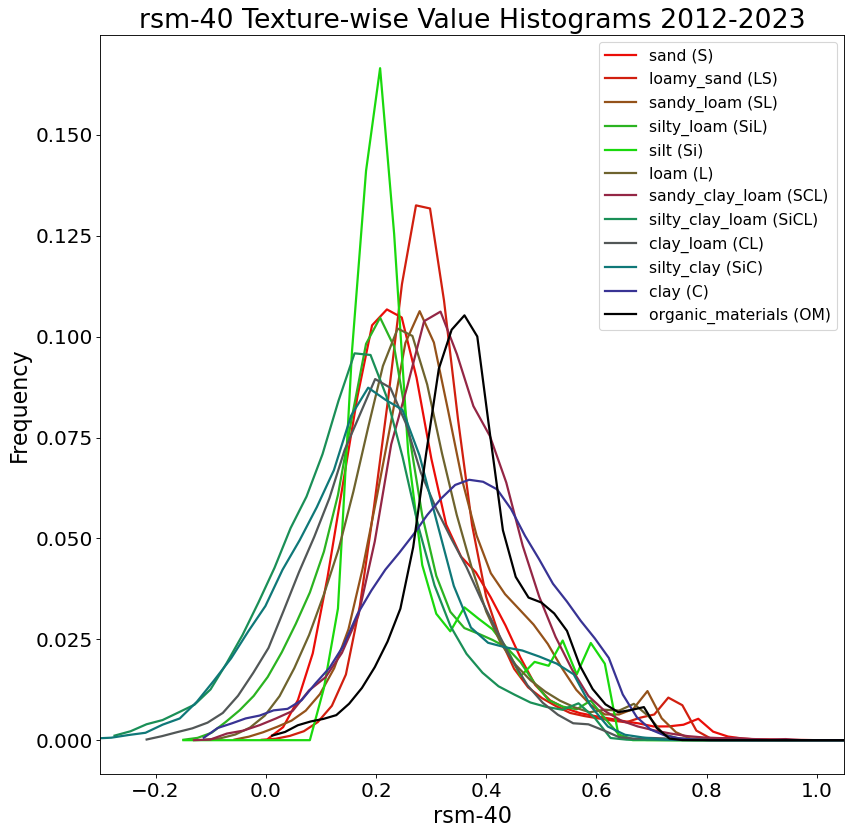
\includegraphics[width=.32\linewidth]{figures/thesis-gridstats/gridstat-hist-textures_rsm-40_2012-1_2023-12_y000-195_x000-462}
    \includegraphics[width=.32\linewidth]{figures/thesis-gridstats/gridstat-hist-textures_rsm-100_2012-1_2023-12_y000-195_x000-462}


    \caption{Distributions of relative soil moisture (top) compared to those of soil moisture area density (bottom) at the first three depth levels, separated by soil texture category. Red, green, and blue components of line colors correspond to the sand, silt, and clay composition of the soil textures, respectively.}
    \label{dist-soilm}
\end{figure}

The differences in conductivity, matric potential, and other hydraulic properties among soil textures causes their distributions to occupy distinct value ranges, and their dynamics to vary at rates that are characteristic to each specific class. As the top row of Figure \ref{gs-rsm} indicates, the distributions of soil moisture area density (in $kg\,m^{-2}$) tends to stratify such that coarser textures (sandy blends) have generally lower moisture content per unit volume, and vice-versa with silt and clay dominant soil textures. Although there is some regional influence, this is mainly owed to the faster percolation rates and lower porosity of the coarser soil.

Since the loss function calculations are directly dependent on the magnitude of soil moisture, we hypothesized that significant differences in these value ranges could diminish the ANNs' ability to learn general solutions that apply to all soil textures. For example, since clay has a slow conductivity and infiltration rate and thus typically smaller magnitudes of increment change, loss calculations based on the increment change would be de-emphasized compared to sand. For this reason, we adopt the relative soil moisture as a physically-interpretable metric for normalizing soil textures to values that occupy roughly the same scale.

\begin{equation}\label{rsm-eq}
    \text{RSM} = \frac{\frac{\text{SOILM}}{d \, \rho_w} - \theta_{wp}}{\theta_s - \theta_{wp}}
\end{equation}

Relative soil moisture (RSM) linearly scales the water content such that each texture's wilting point is at zero, and saturation point corresponds to one. In Equation \ref{rsm-eq}, SOILM is the area density, $\rho_w$ is the density of water, $d$ is the depth of the soil layer, $\theta_s$ is the saturation point of a particular soil texture as a ratio of the total volume, and $\theta_{wp}$ is the wilting point. In this manner, the RSM can never exceed 1, but its lower bound is defined in terms of the hydraulic suction head needed to uptake further water. As such, very dry soils can have RSM values below zero. The layerwise comparisons of SOILM to RSM in Figure \ref{dist-soilm} make clear how RSM normalization aligns the individual texture distributions, and the added benefit of uniting the separate soil layers to a similar range of state values rather than using mass quantities that scale with their unique depths.

\begin{figure}[h!]
    \centering
    \includegraphics[width=.48\linewidth]{figures/thesis-gridstats/gridstat-bulk_rsm-10_2012-1_2023-12_y000-195_x000-462_mean.png}
    \includegraphics[width=.48\linewidth]{figures/thesis-gridstats/gridstat-bulk_rsm-10_2012-1_2023-12_y000-195_x000-462_stdev.png}
    \includegraphics[width=.48\linewidth]{figures/thesis-gridstats/gridstat-bulk_rsm-40_2012-1_2023-12_y000-195_x000-462_mean.png}
    \includegraphics[width=.48\linewidth]{figures/thesis-gridstats/gridstat-bulk_rsm-40_2012-1_2023-12_y000-195_x000-462_stdev.png}
    \includegraphics[width=.48\linewidth]{figures/thesis-gridstats/gridstat-bulk_rsm-100_2012-1_2023-12_y000-195_x000-462_mean.png}
    \includegraphics[width=.48\linewidth]{figures/thesis-gridstats/gridstat-bulk_rsm-100_2012-1_2023-12_y000-195_x000-462_stdev.png}
    \caption{Gridded mean and standard deviation of relative soil moisture (2012-2023).}
    \label{gs-rsm}
\end{figure}

The spatial variation of soil moisture is depicted in Figure \ref{dist-soilm}, which emphasizes several important regional distinctions. The mountainous regions of the West remain rather saturated for much of the year -- especially in the upper soil layers -- owing to their high precipitation rates, the consistent presence of a snow pack, and limited drainage due to frozen soil. Sandy soils tend to have a lower average RSM than other soil types in a particular region due to their high hydraulic conductivity speedy drainage rates. The standard deviations were calculated using the overall per-pixel mean value; as such, clay-dominant soils generally have a higher standard deviation than other textures because their lower conductivity means they take more time to equilibrate after a rain event.

\section{Model Architectures}

The models that we tested fall into three broad architectural categories summarized in the background: fully-connected neural networks (FNNs), na\"ive RNNs, and LSTMs. In this subsection, we will elaborate on the particular implementation of these models for the unique problem structure of this project.

\begin{figure}[h!]
    \centering
    \includegraphics[width=.4\linewidth]{figures/schematic_accfnn.png}
    \caption{Schematic diagram of a multi-layered self-cycling fully connected neural network (FNN).}
    \label{accfnn}
\end{figure}

The basic fully-connected neural network variants we tested are structurally the most similar to Noah-LSM in the sense that the only information passed between time steps are the accumulated magnitudes of soil moisture at each layer given the prediction of the previous layer. As Figure \ref{accfnn} demonstrates, each timestep uses $L$ ANN layers \textbf{A$^(1)$}-\textbf{A$^(L)$} to transform the previous state, current forcing, and static parameter inputs into a prediction for the increment change in state. Only one initial state value $\vec{s}_{-1}$ is needed to run the model since it does not require a multi-step initialization window. The most performant instance of this architecture will serve as a good baseline for understanding the benefit of introducing more structural complexity in the subsequent model types.

\begin{figure}[h!]
    \centering
    \includegraphics[width=.95\linewidth]{figures/schematic_s2s-embed.png}

    \caption{Sequence-to-sequence RNN architecture with initial projection layers \textbf{M}, spin-up window cells \textbf{G} for initializing first-step weights, prediction horizon cells \textbf{E}, and fully-connected decoder layer \textbf{D}.}
    \label{s2s-default}
\end{figure}

The na\"ive RNN and LSTM are distinct from the FNN in that they provide a hidden vector based on past timesteps to supplement the input at each subsequent timestep. In order to initialize the hidden vectors provided to first prediction timestep ($\vec{h}^{(l)}_{init}$ for $l \in [1,\,L]$) with values providing context about the recent history of soil states, we add a spin-up window (\textbf{G}$^{(l)}$) that observes the $W$ timesteps prior to the first prediction and produces a vector for each layer of the output sequence. This principle is diagrammed in Figure \ref{s2s-default}, and applies to both the na\"ive RNN and LSTM. In contrast to the prediction horizon sequence, the spin-up window explicitly receives surface states as inputs, and hidden states of each layer at the final timestep are the only values captured and passed along. For both of these reasons, the spin-up window sequence's weights are not shared with the forecast horizon sequence.

The next architecture we explored was the na\"ive RNN, which has multiple layers of cells that each produce an output based on 3 sets of weights applied to a latent vector from the previous timestep and an input vector from the layer below. The LSTM is similar except that each cell contains 4 sets of weights with outputs that are algebraically combined to produce the output rather than operated upon by a matrix transformation. For further details, refer back to Figure \ref{rnns-both} and Equation \ref{eq_rnn}.

%\begin{figure}[h!]
%    \centering
%    \includegraphics[width=.95\linewidth]{figures/schematic_s2s-accumulator-embed.png}
%
%    \caption{Sequence-to-sequence RNN with explicit output state accumulation.}
%    \label{s2s-accumulator}
%\end{figure}
%
%When the inference algorithm is executed for a multi-layer RNN, every timestep of each layer is evaluated before the hidden states are passed along to a higher-level layer; there is no mechanic for information from the higher layers of previous timesteps to be passed along to the lower layers of subsequent steps. In contrast, the governing equations of Noah-LSM -- including the Richardson equation, plant parameterization, and bare-surface evaporation -- depend very strongly on the magnitude of soil moisture present at any given timestep. As such, we hypothesized that providing an explicit estimate of the soil moisture state as an input at each step would improve prediction skill. As Figure \ref{s2s-accumulator} demonstrates, we implemented this by encapsulating all the layers as a single RNN cell and adding the predicted increment change to the previous state after each step. We will refer to na\"ive RNN and LSTM variants employing this strategy as ``accumulators'', abbreviated as AccRNN and AccLSTM.

All of the models presented here will predict the increment change in state rather than the state magnitude, consistent with the numerical model's estimation of the time derivative as in Equation \ref{dynamical}. Early exploratory testing revealed that models which directly predict the soil state produced very erratic and physically unreasonable results, while predicting increment change led to smoother and more responsive estimates. We suspect that this is because the change in state correlates far more strongly with the current atmospheric forcings than the state magnitude, as many different environmental circumstances could lead to a particular soil state magnitude, but conditions like precipitation, humidity, and temperature have a direct influence on the immediate change in state.

Notice that unlike the numerical model described by Equation \ref{dynamical}, which contains a variable increment change in time $\Delta t$, none of the neural network architectures here have a facility for determining the temporal resolution of predictions they generate. Instead, the coarseness of the timestep is implicit based on the training data, and cannot be changed after training; as such, the coarseness is an independent variable of the training configuration. Unless otherwise specified, the models presented here are all trained at the native 1 hour resolution of the forcing dataset (although the computational timestep of Noah-LSM is 15 minutes), however some models trained at 3 hour or 6 hour resolution showed very promising results. A more thorough analysis of the effect of courser time resolutions on prediction accuracy and model efficiency is left for future work.

\section{Training Paradigm}

One of the main challenges of developing ANNs is contending with the overwhelming number of parameters that can influence model behavior. The modeler must decide on a learning rate schedule, loss function characteristics, the number of layers within the model, the number of trainable weights within each layer, and many other parameters for which there are few reliable standards or heuristics that apply generally to different problem types. To address this, we initially trained 10-25 ANNs within each category while varying multiple parameters between generations based on intuition, and in order to capture a wide breadth of configurations. After these exploratory training runs, we selected the best models from each category and re-trained them while only perturbing one parameter at a time in both directions. For instance, increasing and decreasing the number of layers by one. Finally, the models in each architectural category having the best bulk statistical performance were selected for further more detailed evaluation.

All of the model training was executed on a CPU cluster with 32 cores, and training was allowed to proceed until the prediction skill stopped increasing for a validation dataset (withheld from training) for 48 epochs. In this context, the epoch refers to the number of updates to the model weights between performance reports, which we set to 256. In this environment, training would usually conclude in less than 36 hours. In order to logistically facilitate working with this large number of models, we developed a simple but robust system for storing, deploying, and provisioning data for models based on a set of rigorous configuration standards.

We use functional generators to load, scale, and restructure data on-demand from the source \texttt{timegrid} files during training. This involves extracting sparsely-sampled chunks from multiple files, separating the data into arrays for the spin-up window, prediction horizon inputs, target values, and static data ordered as a set of uniform-length sequences, and linearly normalizing data values so that they approximate a unit gaussian. As mentioned in the beginning of this chapter, it is important to globally shuffle the data used for training in order to avoid over-fitting to a data distribution that only describes a subset of the full domain, so the sequence samples from separate chunks are randomly interleaved. The data generators also accommodate ``derived'' features that are calculated on-demand as a function of the stored features rather than being stored in parallel, which enables target values like RSM or inputs like wind magnitude and relative humidity to be used during training and evaluation without occupying extra disc space and forcing costly re-generation of the \texttt{timegrid} files.

\begin{figure}[h!]
    \centering
    \includegraphics[width=.48\linewidth]{figures/cyclical_lr_logarithmic.png}
    \includegraphics[width=.48\linewidth]{figures/learning-curves_acclstm.png}

    \caption{Learning rate schedule and subsequent learning curves for AccLSTM architectures.}
    \label{learning-rate}
\end{figure}

One of the most important considerations for ANN training setup is the learning rate schedule, which governs the sensitivity of the model's trainable weights to the prediction cost given new data during training. If the learning rate is too high, training may not converge on an optimal solution that relies on fine-grained changes in weights, while if the learning rate is too low, the learning process may take too much time, and could prematurely halt after getting stuck in a local minimum of the loss environment which would require a larger update in model weights to resolve \parencite{russell_artificial_2020}. Practitioners generally start with a high learning rate early in training, and schedule it to gradually decrease as training proceeds \parencite{ren_understanding_2024}, however a separate promising strategy is to cycle between lower and higher learning rates many times \parencite{smith_cyclical_2017}. We mainly utilized a combination of these two methods as shown in the left panel of Figure \ref{learning-rate}, which introduces new tunable parameters including the period of cycles, magnitude of decay, and initial minimum and maximum learning rate.

The loss function is even more critical in determining how the model ultimately behaves, given that it defines the standard for quantifying the skill of predictions. Many applications will simply employ mean absolute error (MAE) or mean squared error (MSE) as the loss metric without further changes, however as long as the functions remains differentiable, modifications can emphasize or de-emphasize certain outputs, balance multiple goals, or assign importance to individual samples based on properties of their data. As such, we tested the effects of manipulating three characteristics of the loss function. First, the values normalized to a unit gaussian in the data generator include the inputs and the target soil moisture state magnitude, however the increment change in soil moisture has its own characteristic distribution that is unique to each soil layer. To address this, we implemented an optional second normalization of increment change values that is only applied within the loss function. In effect, this serves as a coefficient that scales the ratio of the loss associated with each of the output values. Second, the models should prioritize making the locally optimal prediction at each timestep, but they should also be incentivized to recover from error in previous step predictions and produce the globally optimal sequence. To incorporate both of these goals, we introduced a tunable ratio that combines the step-wise error with the integrated state error at each time step. Finally, accurate predictions at some timesteps is considerably more important for producing skillful sequences than many others. For example, a summertime thunderstorm that produces 12cm of precipitation in an hour followed by a two hour surface runoff event will often have a larger influence on the soil column than a subsequent week of drydown near equilibrium. The loss contribution of circumstances like these can be emphasized by adding an additional cost proportional to the true magnitude of change in each layer.

\begin{equation}\label{loss-fn}
    \begin{split}
        L(X',\,Y) &= \rho\,P(X',\text{diff}(Y)) + (1-\rho)\,Q(\text{acc}(X')+Y_{j=0},Y) \\
        P(X',\,Y') &= \frac{1}{S}\,\sum_{i=0}^N \sum_{j=0}^S (1+\gamma \left|Y'_{i,j}\right|)\,\frac{\left|X'_{i,j}-Y'_{i,j}\right|}{\lambda_i} \\
        Q(X,\,Y) &= \frac{1}{S}\,\sum_{i=0}^N \sum_{j=0}^S \left|X_{i,j}-Y_{i,j+1}\right| \\
    \end{split}
\end{equation}


Equation \ref{loss-fn} formalizes the loss function definition for a single pair of prediction ($X$) and target ($Y$) values with $N$ output values (soil layers) and $S$ sequence steps. The arguments to the top-level function $L$ are the $N$ predicted increment changes $X'$, and the $L+1$ true state values (which includes the land surface state immediately prior to the first prediction step). The ``diff'' function is the discrete forward difference along the sequence axis converting the true states to the true increment changes, and the ``acc'' function is the cumulative sum of the predicted changes along the sequence axis. Then $P(X',Y')$ handles the loss contribution of the increment changes, and $Q(X,Y)$ represents that of the state magnitude, which are balanced by the increment loss ratio $\rho$. The $\lambda_i$ parameter serves as the pre-determined normalization coefficient for soil layer $i$, and the magnitude bias parameter $\gamma$ scales the sensitivity of the loss in proportion with the absolute value of the increment change.

\section{Evaluation Metrics}

\begin{equation}
    \label{metric_pcc}
    r(x,y) = \frac{\sum_{i=0}^{N}(x_i-\bar{x})\,(y_i - \bar{y})}{\sqrt{\sum_{i=0}^N(x_i - \bar{x})^2} \cdot \sqrt{\sum_{i=0}^N(y_i-\bar{y})^2}}
\end{equation}

\begin{equation}
    \label{metric_mae}
    MAE(x,y) = \frac{1}{N}\sum_{i=0}^{N}\left|y_i-x_i\right|
\end{equation}

\begin{equation}
    \label{metric_rmse}
    RMSE(x,y) = \sqrt{\frac{1}{N}\sum_{i=0}^{N}\left(y_i-x_i\right)^2}
\end{equation}

The metrics we will use to evaluate the ANN's performance include the pearson correlation coefficient, mean absolute and mean squared error, error bias, as well as entropy-based metrics including information loss and fractional information. The pearson coefficient measures the strength and direction of the linear relationship between variables in terms of the ratio between their covariance and the product of their individual standard deviations. In this case, the variables compared are the target and predicted soil moisture content or the hourly increment change in soil moisture content. A value of 1 would indicate a perfect positive linear relationship, while zero suggests no correlation, and -1 a perfect inverse linear correlation. We calculate the pearson coefficient in accordance with Equation \ref{metric_pcc} independently for each 2-week prediction sequence, then average the results across pixels and initialization times to get the values presented in the following chapter.

Unlike the pearson coefficient, which is scale-invariant, the mean absolute and root mean squared error (MAE, RMSE) metrics present results using the same units as the subject data. MAE is straightforwardly the expected error for a randomly selected target and prediction data pair (Equation \ref{metric_mae}), while RMSE utilizes the average squared difference in data pairs, which makes the metric more sensitive to high-error outliers (Equation \ref{metric_rmse}). Since both of these metrics are differentiable, they can both be used as loss functions while training ANNs. In Equation \ref{loss-fn} -- and by default for most of the models presented here -- we used MAE as the essential form of the loss function, however we will test models trained to optimize the squared error as well.

\begin{figure}[h!]
    \centering
    \includegraphics[width=.54\linewidth,draft=false]{figures/entropy.png}
    \includegraphics[width=.44\linewidth,draft=false]{figures/validation-curves/eval_test_lstm-rsm-9_rsm-10_hist-true-pred_na.png}

    \caption{Entropy curve for a single possible state of a system with respect to the probability of that state being occupied, and an example of a joint histogram validation curve from which the total entropy is calculated.}
    \label{entropy}
\end{figure}

The metrics above all in some way characterize the deviation of the data pairs from a linear relationship. These are straightforward to calculate and especially meaningful for relatively small amounts of data, however for large volumes of data the error rates under the most common conditions can overshadow important characteristics of model behavior in edge cases. As such, when we are considering a large enough volume of data to sufficiently approximate the true distribution of data values, we will also evaluate the ANNs in terms of the uncertainty contribution (also known as information loss) and fractional information according to the methodology used by \parencite{nearing_benchmarking_2016} to the benchmark the uncertainty of Noah-LSM in terms of contributions from the input forcings, model parameters, and model structure. Unlike the correlation coefficient, MAE, and MSE, the fractional information and uncertainty contribution are used to characterize the extent to which using the ANN rather than the source model introduces ambiguity in the distribution of hourly change in RSM by creating a sub-distribution of predictions corresponding to each target. These metrics operate on global properties of the distribution of evaluation results that are less vulnerable to imbalances in the data.

\begin{equation}\label{eq-entropy-h}
    H(z) = - \sum_{i=1}^B \frac{n^{(z)}_i}{N}\ln\left(\frac{n^{(z)}_i}{N}\right) % entropy
\end{equation}

\begin{equation}\label{eq-entropy-i}
    I(y^A,\,y^M) = H(y^M) + H(y^A) - H((y^A,\,y^M)) % mutual information
\end{equation}

The following discussion of the principles and mathematical formalisms from information theory are based on Chapter 2 of Elements of Information Theory \parencite{schilling_entropy_2005}. The information metrics we will use are functions of the Shannon entropy $H(z)$ of the distributions of increment change in RSM, and are estimated in terms of the discrete joint histograms of the targeted and predicted values, such as the one pictured on the right of Figure \ref{entropy}. In Equation \ref{eq-entropy-h}, $n^{(z)}$ represents a histogram of arbitrary variable $z$ with $B$ bins, which counts the integer number of occurrences of data within the value range described by each bin. Each of the bin counts are divided by the total number of observations $N$ to yield the probability of a randomly selected sample occupying that position within the histogram. The integrand function plotted on the left-hand side of Figure \ref{entropy} is applied to the probability associated with each of the bins in order to calculate their individual information contribution to the system, and the total entropy of the distribution is estimated as the sum of the contributions of the bins.

To better understand the properties of a distribution that entropy characterizes, consider a hypothetical distribution that describes a system with a large number of low or zero-probability configurations, and a small number of high-probability configurations. As Figure \ref{entropy} suggests, both the low and high-probability configurations correspond to a relatively small entropy contribution. In contrast, a different hypothetical distribution having probabilities that are spread uniformly across its possible configurations will have a relatively large entropy contribution from each of them, so the sum total entropy of the latter distribution will be higher than the former. In this sense, as described by \parencite{schilling_entropy_2005}: ``the entropy of a random variable is a measure of the uncertainty of the random variable; it is a measure of the amount of information required on the average to describe the random variable''.

Entropy is a fundamental property of a distribution with units of information depending on the base of the logarithmic function used to calculate the integrand. In our case, we use the natural logarithm, which corresponds to ``natural units'' or nats. One of the main advantages of entropy is its chain rule property, which facilitates an additive relationship between the entropy of independent variables and that of their joint distribution. As a consequence, we can straightforwardly calculate the mutual information $I(y^A,\,y^M)$ of two variables, which is a commutative metric of the reduction in uncertainty of one given knowledge of the other. In Equation \ref{eq-entropy-i}, $y^A$ refers to the histogram of increment RSM values predicted by the ANN, $y^M$ to the histogram of Noah-LSM values, and $(y^A,\,y^M)$ to their joint histogram.

\begin{equation}\label{eq-entropy-fi}
    FI(y^A,\,y^M) = \frac{I(y^A,\,y^M)}{H((y^A,\,y^M))} % Fractional Information
\end{equation}

\begin{equation}\label{eq-entropy-u}
    U(y^A;\,y^M) = H(y^A) - I(y^A,\,y^M) % Uncertainty contribution of ANN
\end{equation}

In practice, we will use the entropy and mutual information values to calculate the derived metrics of fractional information ($FI(y^A,\,y^M)$, Equation \ref{eq-entropy-fi}) and uncertainty contribution ($U(y^A;\,y^M)$, Equation \ref{eq-entropy-u}) to characterize the efficiency of the ANNs at emulating the information characteristics of Noah-LSM. Fractional information normalizes the mutual information by the total entropy of the joint distribution, which returns a more familiar ratio value since $H((y^A,\,y^M))$ is a strict upper bound on mutual information. The uncertainty contribution (or information loss) remains in the unit of nats, and explicitly articulates the additional entropy (that is, uncertainty) supplied by employing the ANN rather than the source model.

\chapter{Chapter 4. Results}

\renewcommand{\arraystretch}{0.9}

\section{Exploratory Model Runs}

As mentioned in the previous chapter, one of the main challenges encountered while training neural networks is the overwhelming number of independent variables that can affect model performance. These so-called ``hyperparameters'' may have complex interdependence, and there are few general best-practices. In order to identify a reasonable baseline for the performance of each of the model architectures, we started by training a wide variety of permutations on model properties including the number of layers, nodes per layer, activation function, and prediction coarseness, as well as training properties including loss function characteristics, batch normalization, and weight dropout rate. At this stage, developing a rigorous understanding of the effects of changes in model and training setup was not a priority; instead, we modified multiple hyperparameters simultaneously between training iterations with the goal of establishing rough rules of thumb and a sense for the approximate size of models needed for this task.

\begin{figure}[hp!]
    \centering
    \includegraphics[width=.48\linewidth,draft=false]{figures/efficiency_initial-best/eval_test_efficiency_initial-accfnn-rsm_cc_res.png}
    \includegraphics[width=.48\linewidth,draft=false]{figures/efficiency_initial-best/eval_test_efficiency_initial-accfnn-rsm_cc_state.png}

    \includegraphics[width=.48\linewidth,draft=false]{figures/efficiency_initial-best/eval_test_efficiency_initial-accfnn-rsm_mae_res.png}
    \includegraphics[width=.48\linewidth,draft=false]{figures/efficiency_initial-best/eval_test_efficiency_initial-accfnn-rsm_mae_state.png}

    \includegraphics[width=.48\linewidth,draft=false]{figures/efficiency_initial-best/eval_test_efficiency_initial-accfnn-rsm_mse_res.png}
    \includegraphics[width=.48\linewidth,draft=false]{figures/efficiency_initial-best/eval_test_efficiency_initial-accfnn-rsm_mse_state.png}

    \includegraphics[width=.48\linewidth,draft=false]{figures/efficiency_initial-best/eval_test_efficiency_initial-accfnn-rsm_info-loss_res.png}
    \includegraphics[width=.48\linewidth,draft=false]{figures/efficiency_initial-best/eval_test_efficiency_initial-accfnn-rsm_fi_res.png}

    \caption{Bulk metrics for initial FNN training runs}
    \label{model-init-fnn}
\end{figure}

\begin{table}[H]
\centering
\begin{sideways}
    \begin{tabular}{c|c|c|c|c|c|c }
	\small
Name & Desc & Weights & \thead{State\\MAE} & \thead{State\\CC} & \thead{Info\\Loss} &\thead{Frac.\\Info}\\
\hline
\multirow{3}{6em}{accfnn-rsm-0} & \multirow{3}{16em}{First FNN} & \multirow{3}{4em}{14203} & 0.057 & 0.139 & 2.196 & 0.000 \\ & & & 0.036 & 0.201 & 1.889 & 0.000 \\ & & & 0.020 & -0.215 & 1.694 & 0.000 \\
\hline
\multirow{3}{6em}{accfnn-rsm-1} & \multirow{3}{16em}{Same setup as accrnn-rsm-1 but only a FNN} & \multirow{3}{4em}{14203} & 0.100 & 0.331 & 2.065 & 0.055 \\ & & & 0.032 & 0.517 & 1.840 & 0.024 \\ & & & 0.020 & 0.340 & 1.685 & 0.005 \\
\hline
\multirow{3}{6em}{accfnn-rsm-2} & \multirow{3}{16em}{Much wider and deeper, MSE loss, more dropout} & \multirow{3}{4em}{85947} & 0.064 & -0.139 & 2.193 & 0.001 \\ & & & 0.102 & -0.201 & 1.885 & 0.002 \\ & & & 0.030 & -0.214 & 1.688 & 0.003 \\
\hline
\multirow{3}{6em}{accfnn-rsm-3} & \multirow{3}{16em}{Same as fnn-2 but ignoring constant targets} & \multirow{3}{4em}{85947} & 0.113 & -0.139 & 2.196 & 0.000 \\ & & & 0.034 & 0.201 & 1.889 & 0.000 \\ & & & 0.027 & -0.215 & 1.694 & 0.000 \\
\hline
\multirow{3}{6em}{accfnn-rsm-4} & \multirow{3}{16em}{Same as rsm-2 but no dropout, higher increment magnitude bias} & \multirow{3}{4em}{85947} & 0.042 & 0.786 & 1.530 & 0.181 \\ & & & 0.030 & 0.711 & 1.412 & 0.144 \\ & & & 0.019 & 0.573 & 1.502 & 0.061 \\
\hline
\multirow{3}{6em}{accfnn-rsm-5} & \multirow{3}{16em}{Same as rsm-4 but ignoring constant targets} & \multirow{3}{4em}{85947} & 0.043 & 0.785 & 1.499 & 0.191 \\ & & & 0.029 & 0.688 & 1.411 & 0.143 \\ & & & 0.024 & 0.663 & 1.463 & 0.071 \\
\hline
\multirow{3}{6em}{accfnn-rsm-6} & \multirow{3}{16em}{Same as rsm-4 but narrower and deeper} & \multirow{3}{4em}{30843} & 0.042 & 0.788 & 1.516 & 0.187 \\ & & & 0.027 & 0.692 & 1.423 & 0.142 \\ & & & 0.021 & 0.563 & 1.550 & 0.055 \\
\hline
\multirow{3}{6em}{accfnn-rsm-7} & \multirow{3}{16em}{Same as rsm-6 but mae loss} & \multirow{3}{4em}{30843} & 0.025 & 0.864 & 1.343 & 0.246 \\ & & & 0.014 & 0.831 & 1.242 & 0.219 \\ & & & 0.011 & 0.764 & 1.189 & 0.183 \\
\hline
\multirow{3}{6em}{accfnn-rsm-8} & \multirow{3}{16em}{Same as rsm-7 but ignoring constant targets} & \multirow{3}{4em}{30843} & 0.021 & 0.867 & 1.283 & 0.266 \\ & & & 0.013 & 0.850 & 1.197 & 0.236 \\ & & & 0.011 & 0.809 & 1.154 & 0.196 \\
\hline
\multirow{3}{6em}{accfnn-rsm-9} & \multirow{3}{16em}{fnn 5 but actually using increment norm coefficients} & \multirow{3}{4em}{85947} & 0.050 & 0.738 & 1.632 & 0.151 \\ & & & 0.030 & 0.589 & 1.423 & 0.140 \\ & & & 0.013 & 0.689 & 1.277 & 0.145 \\
    \end{tabular}
\end{sideways}
    \caption{Initial fully-connected neural network properties and bulk statistics.}
    \label{model-init-fnn-table}
\end{table}

All of the bulk statistics in this section are reported in terms of relative soil moisture. The bar charts of correlation coefficient, mean absolute error, and mean squared error separately display the error in hourly increment change and integrated soil state, while the entropy-based metrics (uncertainty contribution and fractional information) are calculated only for the increment change. Tables include metrics for each of the depth levels from top to bottom: 0-10cm, 40-100cm, and 100-200cm.

The validation loss of each of the ANN variants generally stopped decreasing after about 18 hours of training on a CPU, though the training time of individual models unsurprisingly depended most strongly on the size of the model and the learning rate parameters. The models shown here have a number of trainable parameters on the order of 100,000. The best-performing instances of the simplest architecture variant (accfnn-rsm-8) had only about 31,000 parameters and used mean absolute error as the base loss function. The FNN instances struggled to converge any time dropout was used during training, and the predictive skill of best model seemed to improve in the lower two layers in response to a loss function manipulation that ignored prediction cost associated with timesteps where the true magnitude of change in soil moisture state was close to zero. Furthermore, the best FNN did not consider error in state within the loss function (increment loss ratio $\rho = 1$), but was trained with a considerable increment magnitude bias of $\gamma = 60$. The network consisted of 8 fully-connected layers each with 64 nodes.

\begin{figure}[hp!]
    \centering
    \includegraphics[width=.48\linewidth,draft=false]{figures/efficiency_initial-best/eval_test_efficiency_initial-lstm-soilm_cc_res.png}
    \includegraphics[width=.48\linewidth,draft=false]{figures/efficiency_initial-best/eval_test_efficiency_initial-lstm-soilm_cc_state.png}

    \includegraphics[width=.48\linewidth,draft=false]{figures/efficiency_initial-best/eval_test_efficiency_initial-lstm-soilm_mae_res.png}
    \includegraphics[width=.48\linewidth,draft=false]{figures/efficiency_initial-best/eval_test_efficiency_initial-lstm-soilm_mae_state.png}

    \includegraphics[width=.48\linewidth,draft=false]{figures/efficiency_initial-best/eval_test_efficiency_initial-lstm-soilm_mse_res.png}
    \includegraphics[width=.48\linewidth,draft=false]{figures/efficiency_initial-best/eval_test_efficiency_initial-lstm-soilm_mse_state.png}

    \includegraphics[width=.48\linewidth,draft=false]{figures/efficiency_initial-best/eval_test_efficiency_initial-lstm-soilm_info-loss_res.png}
    \includegraphics[width=.48\linewidth,draft=false]{figures/efficiency_initial-best/eval_test_efficiency_initial-lstm-soilm_fi_res.png}

    \caption{Bulk metrics for initial LSTM-VSM training runs}
    \label{model-init-fnn}
\end{figure}

\begin{table}[H]
\begin{sideways}
    \begin{tabular}{c|c|c|c|c|c|c }
    \small
Name & Desc & Weights & \thead{State\\MAE} & \thead{State\\CC} & \thead{Info\\Loss} &\thead{Frac.\\Info}\\
\hline
\multirow{3}{6em}{lstm-1} & \multirow{3}{16em}{4 layers, 64 wide. No batchnorm. } & \multirow{3}{4em}{254397} & 0.107 & 0.509 & 1.686 & 0.138 \\ & & & 0.039 & 0.612 & 1.509 & 0.118 \\ & & & 0.015 & 0.574 & 1.378 & 0.099 \\
\hline
\multirow{3}{6em}{lstm-2} & \multirow{3}{16em}{batchnorm, higher learning rate} & \multirow{3}{4em}{254397} & 0.074 & 0.450 & 1.954 & 0.067 \\ & & & 0.033 & 0.544 & 1.684 & 0.065 \\ & & & 0.020 & 0.360 & 1.507 & 0.057 \\
\hline
\multirow{3}{6em}{lstm-3} & \multirow{3}{16em}{Slower LR ; much 24 wide and 6 layers deep} & \multirow{3}{4em}{64189} & 2.877 & -0.029 & 2.183 & 0.002 \\ & & & 3.153 & -0.084 & 1.873 & 0.002 \\ & & & 0.783 & 0.107 & 1.675 & 0.002 \\
\hline
\multirow{3}{6em}{lstm-4} & \multirow{3}{16em}{4 layers, 96 wide. faster LR, small loss from state magnitude} & \multirow{3}{4em}{629021} & 0.064 & 0.132 & 2.198 & 0.000 \\ & & & 0.049 & 0.196 & 1.882 & 0.002 \\ & & & 0.022 & 0.205 & 1.675 & 0.006 \\
\hline
\multirow{3}{6em}{lstm-8} & \multirow{3}{16em}{4 layers, 64 wide. bigger batch size} & \multirow{3}{4em}{288829} & 0.095 & 0.077 & 2.188 & 0.003 \\ & & & 0.046 & 0.111 & 1.870 & 0.004 \\ & & & 0.029 & -0.034 & 1.671 & 0.003 \\
\hline
\multirow{3}{6em}{lstm-9} & \multirow{3}{16em}{4 layers, 16 wide. bigger batch size} & \multirow{3}{4em}{20029} & 0.076 & 0.035 & 2.195 & 0.000 \\ & & & 0.046 & -0.064 & 1.877 & 0.001 \\ & & & 0.027 & 0.061 & 1.673 & 0.002 \\
\hline
\multirow{3}{6em}{lstm-10} & \multirow{3}{16em}{6 layers, 24 wide; cyclical learning rate ; higher dropout} & \multirow{3}{4em}{65445} & 0.057 & 0.133 & 2.197 & 0.000 \\ & & & 0.034 & 0.127 & 1.882 & 0.000 \\ & & & 0.020 & 0.016 & 1.680 & 0.000 \\
\hline
\multirow{3}{6em}{lstm-11} & \multirow{3}{16em}{2 layers, 256 wide; slower learning rate} & \multirow{3}{4em}{1929597} & 0.066 & 0.286 & 2.058 & 0.039 \\ & & & 0.032 & 0.534 & 1.779 & 0.034 \\ & & & 0.021 & 0.463 & 1.636 & 0.015 \\
\hline
\multirow{3}{6em}{lstm-12} & \multirow{3}{16em}{4 layers, 32 wide; no batchnorm} & \multirow{3}{4em}{74813} & 0.057 & 0.112 & 2.195 & 0.000 \\ & & & 0.037 & -0.193 & 1.880 & 0.001 \\ & & & 0.023 & -0.193 & 1.679 & 0.000 \\
\hline
\multirow{3}{6em}{lstm-13} & \multirow{3}{16em}{same as lstm-12 but increment ratio .8} & \multirow{3}{4em}{74813} & 0.057 & 0.058 & 2.192 & 0.002 \\ & & & 0.034 & 0.055 & 1.879 & 0.001 \\ & & & 0.020 & 0.055 & 1.671 & 0.003 \\
    \end{tabular}
\end{sideways}
    \caption{Initial LSTM-VSM properties and bulk statistics (1).}
    \label{model-init-lstm-table-1}
\end{table}

\begin{table}[H]
\begin{sideways}
    \begin{tabular}{c|c|c|c|c|c|c }
    \small
Name & Desc & Weights & \thead{State\\MAE} & \thead{State\\CC} & \thead{Info\\Loss} &\thead{Frac.\\Info}\\
\hline
\multirow{3}{6em}{lstm-14} & \multirow{3}{16em}{Heavy increment error ; decaying log-cyclical learning rate; batch norm} & \multirow{3}{4em}{74813} & 0.726 & 0.357 & 1.847 & 0.065 \\ & & & 0.224 & 0.416 & 1.565 & 0.067 \\ & & & 0.147 & 0.405 & 1.451 & 0.050 \\
\hline
\multirow{3}{6em}{lstm-15} & \multirow{3}{16em}{No dropout, some increment magnitude bias} & \multirow{3}{4em}{74813} & 1.556 & 0.385 & 1.874 & 0.055 \\ & & & 1.481 & 0.385 & 1.558 & 0.060 \\ & & & 0.831 & 0.352 & 1.407 & 0.052 \\
\hline
\multirow{3}{6em}{lstm-16} & \multirow{3}{16em}{Same as lstm-15 but smaller learning rate} & \multirow{3}{4em}{74813} & 0.032 & 0.826 & 1.258 & 0.276 \\ & & & 0.017 & 0.779 & 1.176 & 0.246 \\ & & & 0.010 & 0.754 & 1.166 & 0.195 \\
\hline
\multirow{3}{6em}{lstm-20} & \multirow{3}{16em}{Stronger dependence on state, some increment magnitude bias, dropout} & \multirow{3}{4em}{77117} & 0.021 & 0.882 & 1.088 & 0.342 \\ & & & 0.013 & 0.884 & 1.036 & 0.309 \\ & & & 0.008 & 0.842 & 1.058 & 0.246 \\
\hline
\multirow{3}{6em}{lstm-21} & \multirow{3}{16em}{lstm-20 but more dropout, more increment magnitude bias, some state loss} & \multirow{3}{4em}{77117} & 0.025 & 0.866 & 1.213 & 0.292 \\ & & & 0.016 & 0.833 & 1.166 & 0.257 \\ & & & 0.011 & 0.762 & 1.191 & 0.189 \\
\hline
\multirow{3}{6em}{lstm-22} & \multirow{3}{16em}{4 layers, 32 wide, faster learning rate} & \multirow{3}{4em}{80221} & 0.035 & 0.823 &  &  \\ & & & 0.020 & 0.816 &  &  \\ & & & 0.013 & 0.737 &  &  \\
\hline
\multirow{3}{6em}{lstm-23} & \multirow{3}{16em}{much smaller encoder, heavier on increment, but less magnitude bias} & \multirow{3}{4em}{43597} & 0.034 & 0.835 &  &  \\ & & & 0.019 & 0.838 &  &  \\ & & & 0.013 & 0.756 &  &  \\
\hline
\multirow{3}{6em}{lstm-24} & \multirow{3}{16em}{64 nodes wide, 5 layers deep; weaker dependence on increment, strong increment magnitude bias} & \multirow{3}{4em}{173165} & 0.035 & 0.821 &  &  \\ & & & 0.018 & 0.840 &  &  \\ & & & 0.013 & 0.735 &  &  \\
\hline
\multirow{3}{6em}{lstm-25} & \multirow{3}{16em}{Same as lstm-24, but 128 nodes wide} & \multirow{3}{4em}{364029} & 0.035 & 0.823 &  &  \\ & & & 0.019 & 0.829 &  &  \\ & & & 0.012 & 0.754 &  &  \\
\hline
\multirow{3}{6em}{lstm-26} & \multirow{3}{16em}{Same as lstm-25, 6 layers deep} & \multirow{3}{4em}{762413} & 0.050 & 0.712 &  &  \\ & & & 0.026 & 0.732 &  &  \\ & & & 0.015 & 0.658 &  &  \\
\hline
\multirow{3}{6em}{lstm-27} & \multirow{3}{16em}{Same as lstm-24, more increment error} & \multirow{3}{4em}{173165} & 0.037 & 0.822 &  &  \\ & & & 0.019 & 0.848 &  &  \\ & & & 0.012 & 0.754 &  &  \\
    \end{tabular}
\centering
\end{sideways}
    \caption{Initial LSTM-VSM properties and bulk statistics (2).}
    \label{model-init-lstm-table-2}
\end{table}

Next, we present a variety of LSTM instances that predict the increment change in volumetric soil moisture (VSM; $\frac{kg}{m^2}$), which we will refer to as the LSTM-VSM group. The results reported here have been converted to relative soil moisture after-the-fact for consistency with the other architectures. In practice, these were the first generations of models we tested; those which appear in Table \ref{model-init-lstm-table-1} were trained using a consistent learning rate and converged rapidly to fairly poor results. Even relatively large models with a variety of hyperparameter configurations didn't achieve a correlation coefficient higher than .65 for any of the layers. Introducing the log-cyclical learning rate schedule prolonged training and, combined with the loss function modifications, resulted in considerably better-performing LSTMs. Given its apparent success, we continued to use the log-cyclical learning rate strategy for the remainder of the models, changing only the rate of decay and the initial minima and maxima of the oscillations. The best LSTM-VSM models we trained had 77,117 trainable weights, a magnitude bias parameter of $\gamma = 10$, increment loss ratio $\rho = .999$, and did not use increment normalization within the loss function. Unlike the FNN architectures, the best LSTM-VSM variants tended to include a small weight dropout of 5\% during training, however without further analysis it is difficult to draw conclusions on the actual impact of any of these changes in isolation.

\begin{figure}[hp!]
    \centering
    \includegraphics[width=.48\linewidth,draft=false]{figures/efficiency_initial-best/eval_test_efficiency_initial-lstm-rsm_cc_res.png}
    \includegraphics[width=.48\linewidth,draft=false]{figures/efficiency_initial-best/eval_test_efficiency_initial-lstm-rsm_cc_state.png}

    \includegraphics[width=.48\linewidth,draft=false]{figures/efficiency_initial-best/eval_test_efficiency_initial-lstm-rsm_mae_res.png}
    \includegraphics[width=.48\linewidth,draft=false]{figures/efficiency_initial-best/eval_test_efficiency_initial-lstm-rsm_mae_state.png}

    \includegraphics[width=.48\linewidth,draft=false]{figures/efficiency_initial-best/eval_test_efficiency_initial-lstm-rsm_mse_res.png}
    \includegraphics[width=.48\linewidth,draft=false]{figures/efficiency_initial-best/eval_test_efficiency_initial-lstm-rsm_mse_state.png}

    \includegraphics[width=.48\linewidth,draft=false]{figures/efficiency_initial-best/eval_test_efficiency_initial-lstm-rsm_info-loss_res.png}
    \includegraphics[width=.48\linewidth,draft=false]{figures/efficiency_initial-best/eval_test_efficiency_initial-lstm-rsm_fi_res.png}

    \caption{Bulk metrics for initial LSTM-RSM (relative soil moisture predictor) training runs}
    \label{model-init-lstm-rsm}
\end{figure}

\begin{table}[H]
\begin{sideways}
    \begin{tabular}{c|c|c|c|c|c|c }
    \small
Name & Desc & Weights & \thead{State\\MAE} & \thead{State\\CC} & \thead{Info\\Loss} &\thead{Frac.\\Info}\\
\hline
\multirow{3}{6em}{lstm-rsm-0} & \multirow{3}{16em}{Small magnitude bias. low dropout. small batch size. 64-wide 4-layer.} & \multirow{3}{4em}{179483} & 0.034 & 0.868 &  &  \\ & & & 0.021 & 0.837 &  &  \\ & & & 0.014 & 0.707 &  &  \\
\hline
\multirow{3}{6em}{lstm-rsm-2} & \multirow{3}{16em}{same as rsm-1, but some state error influence, magnitude bias 30} & \multirow{3}{4em}{179483} & 0.046 & 0.782 &  &  \\ & & & 0.026 & 0.761 &  &  \\ & & & 0.016 & 0.660 &  &  \\
\hline
\multirow{3}{6em}{lstm-rsm-3} & \multirow{3}{16em}{Low dropout, 4 deep, 64 wide decoder, and increment-only loss} & \multirow{3}{4em}{176379} & 0.039 & 0.861 & 1.169 & 0.310 \\ & & & 0.023 & 0.823 & 1.243 & 0.231 \\ & & & 0.015 & 0.677 & 1.285 & 0.152 \\
\hline
\multirow{3}{6em}{lstm-rsm-5} & \multirow{3}{16em}{Same as lstm-rsm-3, but 10\% state influence in loss function} & \multirow{3}{4em}{176379} & 0.057 & 0.133 & 2.206 & 0.000 \\ & & & 0.034 & 0.191 & 1.890 & 0.000 \\ & & & 0.020 & 0.205 & 1.686 & 0.000 \\
\hline
\multirow{3}{6em}{lstm-rsm-6} & \multirow{3}{16em}{Small 3-layer predictor with 100 increment magnitude bias} & \multirow{3}{4em}{48667} & 0.023 & 0.886 & 1.124 & 0.323 \\ & & & 0.017 & 0.805 & 1.149 & 0.261 \\ & & & 0.012 & 0.723 & 1.235 & 0.171 \\
\hline
\multirow{3}{6em}{lstm-rsm-9} & \multirow{3}{16em}{32 nodes wide, 4 layers deep, 10 increment magnitude bias} & \multirow{3}{4em}{48667} & 0.015 & 0.932 & 0.970 & 0.389 \\ & & & 0.009 & 0.922 & 0.941 & 0.352 \\ & & & 0.007 & 0.877 & 0.958 & 0.288 \\
\hline
\multirow{3}{6em}{lstm-rsm-10} & \multirow{3}{16em}{256 nodes wide 5-layer model} & \multirow{3}{4em}{2614907} & 0.138 & 0.168 & 1.671 & 0.159 \\ & & & 0.031 & 0.537 & 1.783 & 0.044 \\ & & & 0.019 & 0.534 & 1.632 & 0.025 \\
%\multirow{3}{6em}{lstm-rsm-11} & \multirow{3}{16em}{same as rsm-9 except coarsened to 3h predictions} & \multirow{3}{4em}{79675} & 0.018 & 0.904 &  &  \\ & & & 0.012 & 0.897 &  &  \\ & & & 0.009 & 0.844 &  &  \\
\hline
\multirow{3}{6em}{lstm-rsm-12} & \multirow{3}{16em}{4 layers deep, 32 nodes wide, steep learning rate decay} & \multirow{3}{4em}{78651} & 0.017 & 0.912 &  &  \\ & & & 0.011 & 0.904 &  &  \\ & & & 0.009 & 0.833 &  &  \\
\hline
\multirow{3}{6em}{lstm-rsm-19} & \multirow{3}{16em}{Single layer 256 nodes wide} & \multirow{3}{4em}{725627} & 0.022 & 0.899 & 1.055 & 0.353 \\ & & & 0.015 & 0.850 & 1.067 & 0.295 \\ & & & 0.010 & 0.806 & 1.086 & 0.227 \\
\hline
\multirow{3}{6em}{lstm-rsm-20} & \multirow{3}{16em}{Same as rsm-19 except some influence of state error} & \multirow{3}{4em}{725627} & 0.023 & 0.899 & 1.048 & 0.356 \\ & & & 0.014 & 0.852 & 1.058 & 0.299 \\ & & & 0.010 & 0.803 & 1.075 & 0.231 \\
    \end{tabular}
\centering
\end{sideways}
    \caption{Initial RSM-normalized LSTM properties and bulk statistics.}
    \label{model-init-lstm-rsm-table}
\end{table}

The next group of models we trained will be referred to as LSTM-RSM models, which have the same structure as the previous set, but target the increment change in RSM rather than volumetric soil moisture. Like the LSTM-VSM models, these seemed to show diminishing returns with model sizes beyond 100,000 weights. The best model we identified has only 48,667 trainable weights, and is 4 layers in depth. Curiously, while the loss function manipulations appeared to have a positive impact on the FNN and LSTM-VSM variants, LSTM-RSM models generally underperformed when a higher magnitude bias and a stronger contribution from the state were used. The best model had a relatively small increment magnitude bias $\gamma=10$, and no contribution from state error ($\rho=1$).


%\begin{figure}[hp!]
%    \centering
%    \includegraphics[width=.48\linewidth,draft=false]{figures/efficiency_initial-best/eval_test_efficiency_initial-acclstm-rsm_cc_res.png}
%    \includegraphics[width=.48\linewidth,draft=false]{figures/efficiency_initial-best/eval_test_efficiency_initial-acclstm-rsm_cc_state.png}
%
%    \includegraphics[width=.48\linewidth,draft=false]{figures/efficiency_initial-best/eval_test_efficiency_initial-acclstm-rsm_mae_res.png}
%    \includegraphics[width=.48\linewidth,draft=false]{figures/efficiency_initial-best/eval_test_efficiency_initial-acclstm-rsm_mae_state.png}
%
%    \includegraphics[width=.48\linewidth,draft=false]{figures/efficiency_initial-best/eval_test_efficiency_initial-acclstm-rsm_mse_res.png}
%    \includegraphics[width=.48\linewidth,draft=false]{figures/efficiency_initial-best/eval_test_efficiency_initial-acclstm-rsm_mse_state.png}
%
%    \caption{Bulk metrics for initial AccLSTM-RSM training runs}
%    \label{model-init-acclstm-rsm}
%\end{figure}
%
%\begin{sidewaystable}
%\begin{center}
%    \begin{tabular}{c|c|c|c|c|c|c }
%    \end{tabular}
%\end{center}
%\end{sidewaystable}


\section{Best Models' Bulk Statistics Comparison}

As Table \ref{model-init-best-table} and Figure \ref{best-metrics} display, the best LSTM-RSM model performed better than the other categories at all of the depth levels, and for each of the evaluation metrics, followed by the LSTM-VSM, and finally the FNN architecture. During evaluation on the full 2018-2023 test dataset, we recorded the execution speed of each of the models as they were applied to multiple subdomains with varying numbers of valid pixels, then fitted a linear regression to the relationship between subdomain size and the time it took to generate a 2-week prediction for each pixel. Evaluation was done with a single CPU thread on a shared high-performance computing cluster. The results in Table \ref{best-exec-efficiency-table} indicate that the initial spin-up time of each model is between 3 and 4 seconds, and execution time for each subsequent pixel is between .1 and 1 millisecond, and is directly proportional to the number of trainable weights in each of the models. When applied to the full domain of 50,875 pixels, the FNN was by far the fastest model at only around 9.5 seconds, while the LSTM variants clocked in at a bit over 40 seconds.

\begin{figure}[hp!]
    \centering
    \includegraphics[width=.48\linewidth,draft=false]{figures/efficiency_initial-best/eval_test_efficiency_initial-best_cc_res.png}
    \includegraphics[width=.48\linewidth,draft=false]{figures/efficiency_initial-best/eval_test_efficiency_initial-best_cc_state.png}

    \includegraphics[width=.48\linewidth,draft=false]{figures/efficiency_initial-best/eval_test_efficiency_initial-best_mae_res.png}
    \includegraphics[width=.48\linewidth,draft=false]{figures/efficiency_initial-best/eval_test_efficiency_initial-best_mae_state.png}

    \includegraphics[width=.48\linewidth,draft=false]{figures/efficiency_initial-best/eval_test_efficiency_initial-best_mse_res.png}
    \includegraphics[width=.48\linewidth,draft=false]{figures/efficiency_initial-best/eval_test_efficiency_initial-best_mse_state.png}

    \includegraphics[width=.48\linewidth,draft=false]{figures/efficiency_initial-best/eval_test_efficiency_initial-best_info-loss_res.png}
    \includegraphics[width=.48\linewidth,draft=false]{figures/efficiency_initial-best/eval_test_efficiency_initial-best_fi_res.png}

    \caption{Bulk metrics comparing the best exploratory models from each category}
    \label{best-metrics}
\end{figure}

\begin{table}[H]
    \centering
    \begin{tabular}{c|c|c|c|c }
        Name & Slope ($ms$) & Intercept ($\frac{s}{px}$) & R$^2$ & Full Domain ($s$) \\
        \hline
        accfnn-rsm-8 & .1262 & 3.088 & .852 & 9.508 \\
        lstm-20 & .8233 & 3.510 & .984 & 45.397 \\
        lstm-rsm-9 & .7544 & 3.246 & .953 & 41.627 \\
    \end{tabular}
    \caption{Linear regression of execution speed for each of the best models.}
    \label{best-exec-efficiency-table}
\end{table}

\begin{table}[H]
    \centering
    \begin{tabular}{c|c|c|c|c|c}
Name &  Weights & \thead{State\\MAE} & \thead{State\\CC} & \thead{Info\\Loss} &\thead{Frac.\\Info}\\
\hline
\multirow{3}{6em}{accfnn-rsm-8} &  \multirow{3}{4em}{30843} & 0.021 & 0.867 & 1.283 & 0.266 \\ & & 0.013 & 0.850 & 1.197 & 0.236 \\ & & 0.011 & 0.809 & 1.154 & 0.196 \\
\hline
\multirow{3}{6em}{lstm-20} &  \multirow{3}{4em}{77117} & 0.021 & 0.882 & 1.088 & 0.342 \\ & & 0.013 & 0.884 & 1.036 & 0.309 \\ & & 0.008 & 0.842 & 1.058 & 0.246 \\
\hline
\multirow{3}{6em}{lstm-rsm-9} & \multirow{3}{4em}{48667} & 0.015 & 0.932 & 0.970 & 0.389 \\ & & 0.009 & 0.922 & 0.941 & 0.352 \\ & & 0.007 & 0.877 & 0.958 & 0.288 \\
    \end{tabular}

    \caption{Size and bulk statistic values of the best models from each category.}
    \label{model-init-best-table}
\end{table}

\begin{figure}[hp!]
    \centering

    \includegraphics[width=.42\linewidth,draft=false]{figures/horizons/eval_best-redo_accfnn-rsm-8_rsm_horizon_na_res.png}
    \includegraphics[width=.42\linewidth,draft=false]{figures/horizons/eval_best-redo_accfnn-rsm-8_rsm_horizon_na_state.png}

    \includegraphics[width=.42\linewidth,draft=false]{figures/horizons/eval_best-redo_lstm-20_rsm_horizon_na_res.png}
    \includegraphics[width=.42\linewidth,draft=false]{figures/horizons/eval_best-redo_lstm-20_rsm_horizon_na_state.png}

    \includegraphics[width=.42\linewidth,draft=false]{figures/horizons/eval_best-redo_lstm-rsm-9_rsm_horizon_na_res.png}
    \includegraphics[width=.42\linewidth,draft=false]{figures/horizons/eval_best-redo_lstm-rsm-9_rsm_horizon_na_state.png}

    %\includegraphics[width=.42\linewidth,draft=false]{figures/horizons/eval_test_acclstm-rsm-4_rsm_horizon_na_res.png}
    %\includegraphics[width=.42\linewidth,draft=false]{figures/horizons/eval_test_acclstm-rsm-4_rsm_horizon_na_state.png}

    \caption{Mean absolute error of each model type with respect to forecast horizon increment (left) and state (right)}
    \label{best-horizons}
\end{figure}

The highest error rates in terms of RSM for each of were associated with the 0-10cm surface layer, which is unsurprising considering that a larger number of processes within Noah-LSM affect the soil dynamics within the topmost layer, which is uniquely influenced by bare-surface evaporation and infiltration from rain and canopy percolation. Furthermore, since the soil layers increase in thickness within Noah-LSM from 10cm at the surface layer to 30cm and 60cm for the deeper layers, each kilogram of actual water mass corresponds to a smaller increment of RSM as it drains downward.

Figure \ref{best-horizons} shows the mean absolute error in RSM for each of the best models with respect to the forecst horizon distance in hours from initialization time. One surprising result that appears universal among the models we trained is that the first few prediction steps consistently have the highest average error in the increment change. For the LSTMs, this could be an indication that the 24 hour spin-up encoder used to initialize the RNN latent vectors prior to the first prediction step have room for improvement, however the FNN has no such encoder. The cause of this spike in error is presently unclear, however in practice, this issue could be mitigated by initializing prediction a few hours prior to the actual initial unknown forecast step, and discarding the first troublesome predictions of increment change.

%\begin{figure}[hp!]
%    \centering
%
%    \includegraphics[width=.32\linewidth,draft=false]{figures/validation-curves/eval_test_accfnn-rsm-8_rsm-10_hist-true-pred_na.png}
%    \includegraphics[width=.32\linewidth,draft=false]{figures/validation-curves/eval_test_accfnn-rsm-8_rsm-40_hist-true-pred_na.png}
%    \includegraphics[width=.32\linewidth,draft=false]{figures/validation-curves/eval_test_accfnn-rsm-8_rsm-100_hist-true-pred_na.png}
%
%    \includegraphics[width=.32\linewidth,draft=false]{figures/validation-curves/eval_test_lstm-20_rsm-10_hist-true-pred_na.png}
%    \includegraphics[width=.32\linewidth,draft=false]{figures/validation-curves/eval_test_lstm-20_rsm-40_hist-true-pred_na.png}
%    \includegraphics[width=.32\linewidth,draft=false]{figures/validation-curves/eval_test_lstm-20_rsm-100_hist-true-pred_na.png}
%
%    \includegraphics[width=.32\linewidth,draft=false]{figures/validation-curves/eval_test_lstm-rsm-9_rsm-10_hist-true-pred_na.png}
%    \includegraphics[width=.32\linewidth,draft=false]{figures/validation-curves/eval_test_lstm-rsm-9_rsm-40_hist-true-pred_na.png}
%    \includegraphics[width=.32\linewidth,draft=false]{figures/validation-curves/eval_test_lstm-rsm-9_rsm-100_hist-true-pred_na.png}
%
%    %\includegraphics[width=.32\linewidth,draft=false]{figures/validation-curves/eval_test_acclstm-rsm-4_rsm-10_hist-true-pred_na.png}
%    %\includegraphics[width=.32\linewidth,draft=false]{figures/validation-curves/eval_test_acclstm-rsm-4_rsm-40_hist-true-pred_na.png}
%    %\includegraphics[width=.32\linewidth,draft=false]{figures/validation-curves/eval_test_acclstm-rsm-4_rsm-100_hist-true-pred_na.png}
%
%    \caption{Heatmaps of true/predicted joint histograms for each of the top 3 soil layers, as predicted by the best models from each category.}
%    \label{best-validation}
%\end{figure}

%\begin{figure}[hp!]
%    \centering
%
%    \includegraphics[width=.32\linewidth,draft=false]{figures/static-combos/eval_test_accfnn-rsm-8_rsm-10_static-combos_abs-err_state.png}
%    \includegraphics[width=.32\linewidth,draft=false]{figures/static-combos/eval_test_accfnn-rsm-8_rsm-40_static-combos_abs-err_state.png}
%    \includegraphics[width=.32\linewidth,draft=false]{figures/static-combos/eval_test_accfnn-rsm-8_rsm-100_static-combos_abs-err_state.png}
%
%    \includegraphics[width=.32\linewidth,draft=false]{figures/static-combos/eval_test_lstm-20_rsm-10_static-combos_abs-err_state.png}
%    \includegraphics[width=.32\linewidth,draft=false]{figures/static-combos/eval_test_lstm-20_rsm-40_static-combos_abs-err_state.png}
%    \includegraphics[width=.32\linewidth,draft=false]{figures/static-combos/eval_test_lstm-20_rsm-100_static-combos_abs-err_state.png}
%
%    \includegraphics[width=.32\linewidth,draft=false]{figures/static-combos/eval_test_lstm-rsm-9_rsm-10_static-combos_abs-err_state.png}
%    \includegraphics[width=.32\linewidth,draft=false]{figures/static-combos/eval_test_lstm-rsm-9_rsm-40_static-combos_abs-err_state.png}
%    \includegraphics[width=.32\linewidth,draft=false]{figures/static-combos/eval_test_lstm-rsm-9_rsm-100_static-combos_abs-err_state.png}
%
%    %\includegraphics[width=.32\linewidth,draft=false]{figures/static-combos/eval_test_acclstm-rsm-4_rsm-10_static-combos_abs-err_state.png}
%    %\includegraphics[width=.32\linewidth,draft=false]{figures/static-combos/eval_test_acclstm-rsm-4_rsm-40_static-combos_abs-err_state.png}
%    %\includegraphics[width=.32\linewidth,draft=false]{figures/static-combos/eval_test_acclstm-rsm-4_rsm-100_static-combos_abs-err_state.png}
%
%    \caption{Absolute error of best models' state from each category with respect to static categorical parameter combinations.}
%    \label{best-static-abserr}
%\end{figure}

%\begin{figure}[hp!]
%    \centering
%
%    \includegraphics[width=.32\linewidth,draft=false]{figures/static-combos/eval_test_accfnn-rsm-8_rsm-10_static-combos_bias_state.png}
%    \includegraphics[width=.32\linewidth,draft=false]{figures/static-combos/eval_test_accfnn-rsm-8_rsm-40_static-combos_bias_state.png}
%    \includegraphics[width=.32\linewidth,draft=false]{figures/static-combos/eval_test_accfnn-rsm-8_rsm-100_static-combos_bias_state.png}
%
%    \includegraphics[width=.32\linewidth,draft=false]{figures/static-combos/eval_test_lstm-20_rsm-10_static-combos_bias_state.png}
%    \includegraphics[width=.32\linewidth,draft=false]{figures/static-combos/eval_test_lstm-20_rsm-40_static-combos_bias_state.png}
%    \includegraphics[width=.32\linewidth,draft=false]{figures/static-combos/eval_test_lstm-20_rsm-100_static-combos_bias_state.png}
%
%    \includegraphics[width=.32\linewidth,draft=false]{figures/static-combos/eval_test_lstm-rsm-9_rsm-10_static-combos_bias_state.png}
%    \includegraphics[width=.32\linewidth,draft=false]{figures/static-combos/eval_test_lstm-rsm-9_rsm-40_static-combos_bias_state.png}
%    \includegraphics[width=.32\linewidth,draft=false]{figures/static-combos/eval_test_lstm-rsm-9_rsm-100_static-combos_bias_state.png}
%
%    %\includegraphics[width=.32\linewidth,draft=false]{figures/static-combos/eval_test_acclstm-rsm-4_rsm-10_static-combos_bias_state.png}
%    %\includegraphics[width=.32\linewidth,draft=false]{figures/static-combos/eval_test_acclstm-rsm-4_rsm-40_static-combos_bias_state.png}
%    %\includegraphics[width=.32\linewidth,draft=false]{figures/static-combos/eval_test_acclstm-rsm-4_rsm-100_static-combos_bias_state.png}
%
%    \caption{Bias of best models' state from each category with respect to static categorical parameter combinations.}
%    \label{best-static-bias}
%\end{figure}

\begin{figure}[hp!]
    \centering

    \includegraphics[width=.48\linewidth,draft=false]{figures/grid-eval_best_full/eval-grid_full_accfnn-rsm-8_rsm-10_spatial-stats_abs-err_state-err-abs-mean.png}
    \includegraphics[width=.48\linewidth,draft=false]{figures/grid-eval_best_full/eval-grid_full_accfnn-rsm-8_rsm-10_spatial-stats_bias_state-err-bias-mean.png}

    \includegraphics[width=.48\linewidth,draft=false]{figures/grid-eval_best_full/eval-grid_full_lstm-20_rsm-10_spatial-stats_abs-err_state-err-abs-mean.png}
    \includegraphics[width=.48\linewidth,draft=false]{figures/grid-eval_best_full/eval-grid_full_lstm-20_rsm-10_spatial-stats_bias_state-err-bias-mean.png}

    \includegraphics[width=.48\linewidth,draft=false]{figures/grid-eval_best_full/eval-grid_full_lstm-rsm-9_rsm-10_spatial-stats_abs-err_state-err-abs-mean.png}
    \includegraphics[width=.48\linewidth,draft=false]{figures/grid-eval_best_full/eval-grid_full_lstm-rsm-9_rsm-10_spatial-stats_bias_state-err-bias-mean.png}

    \caption{Gridded MAE and bias in state for each of the best models at the 0-10cm depth level, evaluated on full test set (2018-2023)}
    \label{grid-full_rsm-10}
\end{figure}

\begin{figure}[hp!]
    \centering

    \includegraphics[width=.48\linewidth,draft=false]{figures/grid-eval_best_full/eval-grid_full_accfnn-rsm-8_rsm-40_spatial-stats_abs-err_state-err-abs-mean.png}
    \includegraphics[width=.48\linewidth,draft=false]{figures/grid-eval_best_full/eval-grid_full_accfnn-rsm-8_rsm-40_spatial-stats_bias_state-err-bias-mean.png}

    \includegraphics[width=.48\linewidth,draft=false]{figures/grid-eval_best_full/eval-grid_full_lstm-20_rsm-40_spatial-stats_abs-err_state-err-abs-mean.png}
    \includegraphics[width=.48\linewidth,draft=false]{figures/grid-eval_best_full/eval-grid_full_lstm-20_rsm-40_spatial-stats_bias_state-err-bias-mean.png}

    \includegraphics[width=.48\linewidth,draft=false]{figures/grid-eval_best_full/eval-grid_full_lstm-rsm-9_rsm-40_spatial-stats_abs-err_state-err-abs-mean.png}
    \includegraphics[width=.48\linewidth,draft=false]{figures/grid-eval_best_full/eval-grid_full_lstm-rsm-9_rsm-40_spatial-stats_bias_state-err-bias-mean.png}

    \caption{Gridded MAE and bias in state for each of the best models at the 10-40cm depth level, evaluated on full test set (2018-2023)}
    \label{grid-full_rsm-40}
\end{figure}

\begin{figure}[hp!]
    \centering

    \includegraphics[width=.48\linewidth,draft=false]{figures/grid-eval_best_full/eval-grid_full_accfnn-rsm-8_rsm-100_spatial-stats_abs-err_state-err-abs-mean.png}
    \includegraphics[width=.48\linewidth,draft=false]{figures/grid-eval_best_full/eval-grid_full_accfnn-rsm-8_rsm-100_spatial-stats_bias_state-err-bias-mean.png}

    \includegraphics[width=.48\linewidth,draft=false]{figures/grid-eval_best_full/eval-grid_full_lstm-20_rsm-100_spatial-stats_abs-err_state-err-abs-mean.png}
    \includegraphics[width=.48\linewidth,draft=false]{figures/grid-eval_best_full/eval-grid_full_lstm-20_rsm-100_spatial-stats_bias_state-err-bias-mean.png}

    \includegraphics[width=.48\linewidth,draft=false]{figures/grid-eval_best_full/eval-grid_full_lstm-rsm-9_rsm-100_spatial-stats_abs-err_state-err-abs-mean.png}
    \includegraphics[width=.48\linewidth,draft=false]{figures/grid-eval_best_full/eval-grid_full_lstm-rsm-9_rsm-100_spatial-stats_bias_state-err-bias-mean.png}

    \caption{Gridded MAE and bias in state for each of the best models at the 40-100cm depth level, evaluated on full test set (2018-2023)}
    \label{grid-full_rsm-100}
\end{figure}

Figures \ref{grid-full_rsm-10}, \ref{grid-full_rsm-40}, and \ref{grid-full_rsm-100} show the overall spatial distribution of mean absolute error and model bias at the 0-10cm, 10-40cm, and 40-100cm depth levels, respectively. We will use the information that these graphics provide to identify areas of anomalous model behavior for further investigation in the following section.

The LSTM-RSM shows a widespread slight dry bias in the surface layer with the exception of urban areas, mountainous regions, and some sandy areas in Texas, New Mexico, and the Northern Midwest. The LSTM-VSM (lstm-20) largely follows suit, though it also showed regions of wet bias where the LSTM-RSM was more neutral or dry including silty regions corresponding to the Ouachita mountains, central Kentucky and the Cumberland plateu, the Northern Rockies in Idaho and Montana, and Florida. The FNN model had significantly more of a wet bias in the surface layer for some regions, which were largely distinguished discretely by their soil texture boundaries.

All three models had more of a mixture of wet and dry biases in the 10-40cm layer. In the Midwest, Northern Wisconson and Minnesota were dry except for isolated sandy pixels, while the cropland in the Ohio and Missouri River basins to the South and West of that region were notably too wet: a pattern that was further emphasized in the 40-100cm layer. The wet bias associated with the cropland surface type was also apparent in Mississippi Alluvial Plains of Eastern Arkansas and the Missouri Bootheel, discrete regions of East Texas, the Florida Penninsula, and East-central South Carolina. Furthermore, each of the models also demonstrated a wet bias associated with clay-dominant pixels in the Centeral Texas and surrounding the Southern extent of the Mississippi River. In addition to the Northeast and Northern Midwest, the regions with the most significant dry bias in the lower two layers seemed to be associated with higher elevation, especially the Sierra Nevada mountains, Colorado Rockies, and Central Idaho, although the Cascades seem to be an exception with a stark wet bias for the LSTM-RSM model.

\begin{figure}[h!]
    \centering
    \includegraphics[width=.66\linewidth,draft=false]{figures/static_slopetype_3km.png}
    \caption{SLOPETYPE classes defining bottom-layer drainage.}
    \label{slopetype-classes}
\end{figure}

In the lower two layers, there is also an anomalous tiling artifact present in the model biases that is especially noticable in the Ohio river valley, Montana, and the central Great Plains. The emerging squares are 8 pixels in length and width, forming a $1^\circ$ grid. This was initially perplexing since no similar pattern appears in the forcings, however close inspection of the mean Noah-LSM soil moisture content in 40-100cm layer of Figure \ref{gs-rsm} also reveals subtle edges that correspond to the bias tiles. Upon further investigation, we found that the square boundaries closely align with an input parameter in Noah-LSM called SLOPETYPE which controls the rate at which water drains out of the lowest layer of the model by applying one of 9 discrete classes \citep{mitchell_community_2005}, which are displayed by Figure \ref{slopetype-classes}. This parameter is distinct from the surface slope (which is defined in terms of degrees from vertical), and wasn't provided as an input to the ANNs during training, so the patterns in model bias are emergent from the unexplained variance introduced by leaving out these values.

Despite the inconsistencies between the models' biases, several regions stand out as especially troublesome in terms of all of the models' mean absolute error. Sandy areas in the Midwest, Nebraska, Oregon, and the Four Corners region of the Desert Southwest have high error rates in the first two layers. In the 40-100cm layer, clay pixels in Mississippi, Louisiana, Alabama, and Northern Ohio suffer, and the Sierra Nevada and Cascade mountains proved especially difficult for the models to characterize in the lower two soil layers.

%\begin{figure}[hp!]
%    \centering
%
%    \includegraphics[width=.96\linewidth,draft=false]{figures/grid-eval_best_full/eval-grid_full_lstm-rsm-9_rsm-10_hist-humidity-temp_abs-err.png}
%    \includegraphics[width=.96\linewidth,draft=false]{figures/grid-eval_best_full/eval-grid_full_lstm-rsm-9_rsm-10_hist-humidity-temp_bias.png}
%
%    \caption{Joint histogram of humidity and temperature forcings, with mean absolute error (top) and error bias (bottom) plotted within corresponding bins.}
%    \label{lstm-rsm-9-hthist}
%\end{figure}

%\begin{figure}[hp!]
%    \centering
%
%    \includegraphics[width=.96\linewidth,draft=false]{figures/grid-eval_best_full/eval-grid_full_lstm-rsm-9_rsm-10_hist-state-increment_abs-err.png}
%    \includegraphics[width=.96\linewidth,draft=false]{figures/grid-eval_best_full/eval-grid_full_lstm-rsm-9_rsm-10_hist-state-increment_bias.png}
%
%    \caption{Joint histogram of total RSM and increment change of RSM in the 0-10cm layer, with mean absolute error (top) and error bias (bottom) plotted within corresponding bins.}
%    \label{lstm-rsm-9-sihist-rsm-10}
%\end{figure}

%\begin{figure}[hp!]
%    \centering
%
%    \includegraphics[width=.96\linewidth,draft=false]{figures/grid-eval_lstm-rsm-9_full/eval-grid_full_lstm-rsm-9_rsm-40_hist-state-increment_abs-err.png}
%    \includegraphics[width=.96\linewidth,draft=false]{figures/grid-eval_lstm-rsm-9_full/eval-grid_full_lstm-rsm-9_rsm-40_hist-state-increment_bias.png}
%
%    \caption{Joint histogram of total RSM and increment change of RSM in the 10-40cm layer, with mean absolute error (top) and error bias (bottom) plotted within corresponding bins.}
%    \label{lstm-rsm-9-sihist-rsm-40}
%\end{figure}

%\begin{figure}[hp!]
%    \centering
%
%    \includegraphics[width=.96\linewidth,draft=false]{figures/grid-eval_lstm-rsm-9_full/eval-grid_full_lstm-rsm-9_rsm-100_hist-state-increment_abs-err.png}
%    \includegraphics[width=.96\linewidth,draft=false]{figures/grid-eval_lstm-rsm-9_full/eval-grid_full_lstm-rsm-9_rsm-100_hist-state-increment_bias.png}
%
%    \caption{Joint histogram of total RSM and increment change of RSM in the 40-100cm layer, with mean absolute error (top) and error bias (bottom) plotted within corresponding bins.}
%    \label{lstm-rsm-9-sihist-rsm-100}
%\end{figure}

\section{Spatial, Temporal, and Situational Evaluation}

From this point forward in our analysis of the results we will focus exclusively on the best overall model, ``lstm-rsm-9'', with the goal of better understanding its performance in a variety of regional and meteorological scenarios.

\begin{figure}[h!]
    \centering

    \includegraphics[width=.99\linewidth,draft=false]{figures/seq-eval_lstm-rsm-9/eval-grid_full_lstm-rsm-9_rsm-10_hist-humidity-temp_all-3.png}

    \caption{Joint histogram between temperature and absolute humidity (left) with increment mean absolute error (center) and bias (right) for the 0-10cm layer in corresponding bins (lstm-rsm-9; 2018-2023).}
    \label{bulk-eval_humidity-temp}
\end{figure}

Figure \ref{bulk-eval_humidity-temp} demonstrates the model's performance at the surface layer with respect to the atmospheric temperature and humidity at each of the hourly prediction times. This includes data from all pixels within the CONUS domain throughout the test period from 2018 to 2023 inclusively. A few features stand out immediately: the highest overall error rates were associated with air near saturation and above freezing, which represent a strong dry bias. The removal water from surface layer by plant transpiration and bare-surface evaporation is limited by the potential evaporation given by the Penman relationship as estimated in the formulation from \citep{mahrt_influence_1984}, which is inversely related to the relative humidity. As the air approaches saturation, the potential evaporation diminishes to only include a term dependent on the difference between the net radiation at the surface and the flux of heat to the soil, which is negative during the night time. As such, one possible explanation for the cause of error near saturation is that the ANNs are insufficient at accounting for the discrete halting of evapotranspiration under these atmospheric conditions, which would lead to unrealistic removal of water from the soil column and a subsequent dry bias like the one observed.

It is also important to recognize that regional meteorology can create hidden factors that must be considered in the interpretation of a forcing histogram like this one. For example, very warm and saturated air is considerably more common in the South and Southeast US as Figure \ref{gs-forcings} suggests, so the corresponding areas in Figure \ref{bulk-eval_humidity-temp} will be dominated by a subset of pixels from those regions. It is difficult to marginalize over all of these variables, so further analysis is needed to draw confident conclusions about model behavior.

\begin{figure}[hp!]
    \centering

    \includegraphics[width=.99\linewidth,draft=false]{figures/seq-eval_lstm-rsm-9/eval-grid_full_lstm-rsm-9_rsm-10_hist-state-increment_bias.png}

    \includegraphics[width=.99\linewidth,draft=false]{figures/seq-eval_lstm-rsm-9/eval-grid_full_lstm-rsm-9_rsm-40_hist-state-increment_bias.png}

    \includegraphics[width=.99\linewidth,draft=false]{figures/seq-eval_lstm-rsm-9/eval-grid_full_lstm-rsm-9_rsm-100_hist-state-increment_bias.png}

    \caption{Joint histogram between target increment change in RSM and RSM magnitude (left) with increment bias (right) in corresponding bins at each depth level (lstm-rsm-9; 2018-2023).}
    \label{bulk-eval_state-increment}
\end{figure}

Now consider Figure \ref{bulk-eval_state-increment}, which demonstrates how the bias in increment change is related to the RSM and rate of change of RSM throughout the test period. A dominant pattern in all of the soil layers and for all of the models we tested is that the magnitude of wetting and drying rates were both mainly under-estimated. That is, when the RSM in a layer was decreasing, the predicted rate of decrease was too slow, and when RSM was increasing, the models' predictions for the increment change were too low. This effect is more severe as the magnitude of the increment change increases in either direction.

\begin{figure}[h!]
    \centering
    \includegraphics[width=.99\linewidth,draft=false]{figures/grid-eval_qtrly/eval-grid_full_lstm-rsm-9_pixelwise-time-stats_monthly-txtr-abs-err-state-rsm-10.png}

    \caption{Overall monthly mean bias in RSM state at each depth level (lstm-rsm-9; 2018-2023)}
    \label{bulk-eval_monthly-txtr-error}
\end{figure}

Let us now consider how model performance is related to seasonal change. Figure \ref{bulk-eval_monthly-txtr-error} shows how the mean error rates vary seasonally for each unique soil texture in the 0-10cm layer, and Figure \ref{bulk-eval_qtrly_rsm-10} separates the spatial plots of mean absolute error and bias for the same layer into seasonal groupings that are averaged over all six years in the test period. In the surface layer during the winter, sand and loamy sand texture dominate much of the error, most notably in Michigan, upper Nebraska, and in sand-dominant regions scattered throughout the desert west like Central Washington, the Navajo Nation, and West Texas. Nonetheless, other sandy regions with warmer climates like Southeast Texas and Florida didn't see significantly degraded performance during the winter season, which leads us to suspect that the model struggles to capture the dynamics of frozen or partially-frozen sandy soil. In general, these high-error regions correspond to a wet bias, with the notable exception of the Nebraska sand hills.

\begin{figure}[h!]
    \centering
    \includegraphics[width=.99\linewidth,draft=false]{figures/grid-eval_qtrly/eval-grid_full_lstm-rsm-9_pixelwise-time-stats_monthly-elev-abs-err-state-rsm-10.png}

    \includegraphics[width=.99\linewidth,draft=false]{figures/grid-eval_qtrly/eval-grid_full_lstm-rsm-9_pixelwise-time-stats_monthly-elev-bias-state-rsm-10.png}

    \caption{Monthly absolute error (top) and error bias (bottom) in the 0-10cm layer (lstm-rsm-9; 2018-2023)}
    \label{bulk-eval_monthly-elev-err_0-10cm}
\end{figure}


\begin{figure}[hp!]
    \centering

    \includegraphics[width=.99\linewidth,draft=false]{figures/grid-eval_qtrly/eval-grid_full_lstm-rsm-9_pixelwise-time-stats_abs-err_qtrly-err-state-rsm-10.png}

    %\includegraphics[width=.99\linewidth,draft=false]{figures/grid-eval_qtrly/eval-grid_full_lstm-rsm-9_pixelwise-time-stats_abs-err_qtrly-err-state-rsm-10-mape.png}

    \includegraphics[width=.99\linewidth,draft=false]{figures/grid-eval_qtrly/eval-grid_full_lstm-rsm-9_pixelwise-time-stats_bias_qtrly-err-state-rsm-10.png}

    \caption{Quarterly mean absolute error (top) and bias (bottom) for the 0-10cm layer (lstm-rsm-9; 2018-2023).}
    \label{bulk-eval_qtrly_rsm-10}
\end{figure}

The 0-10cm layer also showed error maxima on either side of the Cascade and Sierra Nevada mountain ranges, however as Figure \ref{bulk-eval_monthly-elev-err_0-10cm} suggests, this winter error maximum was limited to altitudes in the range of about 1,000-2,500ft. The highest peaks above 2,500ft showed lower average error rates than at all other altitudes during this period of time. Moving into the spring season, however, this situation reverses such that the average absolute error rates are significantly higher going up in altitude. By May, the high peaks exhibit a strong wet bias that persists but gradually wanes through the summer and fall seasons.

\begin{figure}[h!]
    \centering

    \includegraphics[width=.99\linewidth,draft=false]{figures/grid-eval_qtrly/eval-grid_full_lstm-rsm-9_pixelwise-time-stats_abs-err_qtrly-horizon-apcp.png}

    \caption{Quarterly mean precipitation distribution during the test period ($\frac{cm}{hr}$; 2018-2023).}
    \label{bulk-eval_qtrly-precip}
\end{figure}

Figure \ref{bulk-eval_qtrly-precip} shows that the highest average precipitation rates observed anywhere within the domain fall on the Sierra Nevadas, Cascades, and the Northwest Coast during the winter season. At high altitudes, this will almost invariable be in the form of snow, which is not immediately infiltrated into the soil column. This suggests that the high error rates observed in the foothills during the winter and subsequently on the mountain peaks in the spring may be associated with the freezing and thawing processes or snow pack melting rather than snowfall itself.

While some sandy regions in Nebraska and the Midwest still exhibit high error rates in the surface layer during the spring season, clay-dominant soils begin to cause more issues moving into the Summer, especially in the South surrounding the Mississippi river and in Central/Southeastern Texas reliably associated with a wet bias, which is reflected in the time series from Figure \ref{bulk-eval_qtrly_rsm-10}. Similarly, pixels with urban surface types begin standing out with high error rates and a stark wet bias in the 0-10cm layer regardless of their soil texture. During the fall, the highest error rates in the surface layer were associated with a wet bias in the tallest peaks of the Sierra Nevadas and Colorado Rockies, along with the troublesome Nebraska sand hills. Notice that Figure \ref{bulk-eval_monthly-elev-err_0-10cm} shows two distinct error maxima associated with high altitudes in the spring and fall. If the snow and soil freeze-thaw process is indeed responsible for the high error rates observed in the mountains, the maximum in the fall is likely to be associated with the first transient snowfall events late in the season.


\begin{figure}[hp!]
    \centering

    \includegraphics[width=.99\linewidth,draft=false]{figures/grid-eval_qtrly/eval-grid_full_lstm-rsm-9_pixelwise-time-stats_abs-err_qtrly-err-state-rsm-40.png}

    %\includegraphics[width=.99\linewidth,draft=false]{figures/grid-eval_qtrly/eval-grid_full_lstm-rsm-9_pixelwise-time-stats_abs-err_qtrly-err-state-rsm-40-mape.png}

    \includegraphics[width=.99\linewidth,draft=false]{figures/grid-eval_qtrly/eval-grid_full_lstm-rsm-9_pixelwise-time-stats_bias_qtrly-err-state-rsm-40.png}

    \caption{Quarterly mean absolute error (top) and bias (bottom) for the 10-40cm layer (lstm-rsm-9; 2018-2023).}
    \label{bulk-eval_qtrly_rsm-40}
\end{figure}

As Figure \ref{bulk-eval_qtrly_rsm-40} displays, the 10-40cm layer also saw relatively high error rates during the winter associated with the sandy regions mentioned previously including the Four Corners region of the Desert West and Northern Michigan. There were also winter error maxima associated with the mountainous regions of Washington, Oregon, and California with a strong wet bias in the Cascades and Northern Coast Ranges, which contrasted a stark dry bias in the southern extent of the Sierra Nevadas. Curiously, the Colorado Rockies performed very well during the same time frame compared to the surrounding regions.

\begin{figure}[h!]
    \centering

    \includegraphics[width=.99\linewidth,draft=false]{figures/grid-eval_qtrly/eval-grid_full_lstm-rsm-9_pixelwise-time-stats_abs-err_qtrly-horizon-tmp.png}

    \caption{Quarterly mean air temperature during the test period (2018-2023)}
    \label{bulk-eval_qtrly_temp}
\end{figure}

During the winter in the 10-40cm layer, also consider the widespread meridional band of higher error rates around 0.02 RSM which spans a variety of soil textures from Missouri through the Midwest, Kentucky, West Virginia and Pennsylvania. This area is bounded by regions of lower average error to the North in the High Plains and Wisconsin, and broadly in the South and Southeast. Moving into the spring time frame, similar high error rates seem to migrate northward, resulting in error similarly spanning soil textures in Wisconsin, Minnesota, and the Dakotas. This may be owed in part to the northward movement of the latitude at which the air temperature more commonly fluctuates above and below freezing as winter gives way to spring. Such fluctuations complicate the soil freezing and thawing process, and Figure \ref{bulk-eval_qtrly_temp} suggests that the freezing line of the average air temperature seasonally expands and recedes over this area. Another factor may be the higher precipitation rates in those regions evident from Figure \ref{bulk-eval_qtrly-precip}, or a combination of the two.

\begin{figure}[h!]
    \centering

    \includegraphics[width=.99\linewidth,draft=false]{figures/grid-eval_qtrly/eval-grid_full_lstm-rsm-9_pixelwise-time-stats_monthly-txtr-bias-state-rsm-40.png}

    \caption{Monthly mean bias in 10-40cm RSM with respect to soil texture ($\frac{cm}{hr}$; 2018-2023).}
    \label{bulk-eval_monthly_txtr-bias}
\end{figure}

\begin{figure}[hp!]
    \centering

    \includegraphics[width=.99\linewidth,draft=false]{figures/grid-eval_qtrly/eval-grid_full_lstm-rsm-9_pixelwise-time-stats_abs-err_qtrly-err-state-rsm-100.png}

    %\includegraphics[width=.99\linewidth,draft=false]{figures/grid-eval_qtrly/eval-grid_full_lstm-rsm-9_pixelwise-time-stats_abs-err_qtrly-err-state-rsm-100-mape.png}

    \includegraphics[width=.99\linewidth,draft=false]{figures/grid-eval_qtrly/eval-grid_full_lstm-rsm-9_pixelwise-time-stats_bias_qtrly-err-state-rsm-100.png}

    \caption{Quarterly mean absolute error (top) and bias (bottom) for the 40-100cm layer (lstm-rsm-9; 2018-2023).}
    \label{bulk-eval_qtrly_rsm-100}
\end{figure}

\newpage

\section{Parameter and Loss Function Variations}

\begin{figure}[hp!]
    \centering
    \includegraphics[width=.48\linewidth,draft=false]{figures/efficiency_variations/eval_test_efficiency_variations-feat-lstm-rsm-9_cc_res.png}
    \includegraphics[width=.48\linewidth,draft=false]{figures/efficiency_variations/eval_test_efficiency_variations-feat-lstm-rsm-9_cc_state.png}

    \includegraphics[width=.48\linewidth,draft=false]{figures/efficiency_variations/eval_test_efficiency_variations-feat-lstm-rsm-9_mae_res.png}
    \includegraphics[width=.48\linewidth,draft=false]{figures/efficiency_variations/eval_test_efficiency_variations-feat-lstm-rsm-9_mae_state.png}

    \includegraphics[width=.48\linewidth,draft=false]{figures/efficiency_variations/eval_test_efficiency_variations-feat-lstm-rsm-9_mse_res.png}
    \includegraphics[width=.48\linewidth,draft=false]{figures/efficiency_variations/eval_test_efficiency_variations-feat-lstm-rsm-9_mse_state.png}

    \includegraphics[width=.48\linewidth,draft=false]{figures/efficiency_variations/eval_test_efficiency_variations-feat-lstm-rsm-9_info-loss_res.png}
    \includegraphics[width=.48\linewidth,draft=false]{figures/efficiency_variations/eval_test_efficiency_variations-feat-lstm-rsm-9_fi_res.png}

    \caption{Bulk metrics for initial FNN training runs}
    \label{model-init-fnn}
\end{figure}

\begin{table}[H]
\centering
    \begin{tabular}{c|c|c|c|c|c }
    \small
Name & \thead{Feature \\ Negated} &  \thead{State\\MAE} & \thead{State\\CC} & \thead{Info\\Loss} &\thead{Frac.\\Info}\\
\hline
\multirow{3}{6em}{lstm-rsm-9} & \multirow{3}{8em}{Initial Best LSTM-RSM} & 0.015 & 0.932 & 0.970 & 0.389 \\ & & 0.009 & 0.922 & 0.941 & 0.352 \\ & & 0.007 & 0.877 & 0.958 & 0.288 \\
\hline
\multirow{3}{6em}{lstm-rsm-34} & \multirow{3}{8em}{Leaf Area Index} & 0.013 & 0.942 & 0.927 & 0.406 \\ & & 0.008 & 0.915 & 0.916 & 0.364 \\ & & 0.007 & 0.888 & 0.946 & 0.294 \\
\hline
\multirow{3}{6em}{lstm-rsm-35} & \multirow{3}{8em}{Green Vegetation Fraction} & 0.016 & 0.931 & 1.000 & 0.372 \\ & & 0.009 & 0.918 & 0.954 & 0.346 \\ & & 0.008 & 0.855 & 1.003 & 0.268 \\
\hline
\multirow{3}{6em}{lstm-rsm-36} & \multirow{3}{8em}{Temperature} & 0.016 & 0.925 & 1.007 & 0.372 \\ & & 0.010 & 0.912 & 0.964 & 0.339 \\ & & 0.007 & 0.880 & 0.970 & 0.280 \\
\hline
\multirow{3}{6em}{lstm-rsm-37} & \multirow{3}{8em}{Humidity} & 0.013 & 0.938 & 0.968 & 0.389 \\ & & 0.009 & 0.919 & 0.942 & 0.352 \\ & & 0.007 & 0.884 & 0.991 & 0.273 \\
\hline
\multirow{3}{6em}{lstm-rsm-38} & \multirow{3}{8em}{Pressure} & 0.014 & 0.936 & 0.938 & 0.402 \\ & & 0.008 & 0.919 & 0.925 & 0.361 \\ & & 0.007 & 0.860 & 0.917 & 0.306 \\
\hline
%\multirow{3}{6em}{lstm-rsm-39} & \multirow{3}{8em}{Wind Magnitude} & 0.014 & 0.940 & 0.942 & 0.401 \\ & & 0.009 & 0.922 & 0.948 & 0.352 \\ & & 0.007 & 0.882 & 0.973 & 0.280 \\
\multirow{3}{6em}{lstm-rsm-39} & \multirow{3}{8em}{Wind Magnitude} & 0.015 & 0.937 & 0.972 & 0.387 \\ & & 0.009 & 0.922 & 0.932 & 0.355 \\ & & 0.007 & 0.892 & 0.964 & 0.284 \\
\hline
\multirow{3}{6em}{lstm-rsm-40} & \multirow{3}{8em}{Downward LW Radiation} & 0.015 & 0.925 & 1.012 & 0.371 \\ & & 0.009 & 0.916 & 0.955 & 0.343 \\ & & 0.007 & 0.890 & 0.949 & 0.289 \\
\end{tabular}
    \caption{Bulk statistic results for lstm-rsm-9 variants trained with individual features excluded (1)}
    \label{feat-variants-table-1}
\end{table}

\begin{table}[H]
    \centering
    \begin{tabular}{c|c|c|c|c|c }
    \small
Name & \thead{Feature \\ Negated} & \thead{State\\MAE} & \thead{State\\CC} & \thead{Info\\Loss} &\thead{Frac.\\Info}\\
\hline
\multirow{3}{6em}{lstm-rsm-9} & \multirow{3}{8em}{Initial Best LSTM-RSM} & 0.015 & 0.932 & 0.970 & 0.389 \\ & & 0.009 & 0.922 & 0.941 & 0.352 \\ & & 0.007 & 0.877 & 0.958 & 0.288 \\
\hline
\multirow{3}{6em}{lstm-rsm-41} & \multirow{3}{8em}{Downward SW Radiation} & 0.016 & 0.923 & 1.072 & 0.347 \\ & & 0.009 & 0.914 & 0.967 & 0.338 \\ & & 0.007 & 0.877 & 0.962 & 0.284 \\
\hline
\multirow{3}{6em}{lstm-rsm-42} & \multirow{3}{8em}{Precipitation} & 0.088 & 0.348 & 1.621 & 0.167 \\ & & 0.029 & 0.590 & 1.448 & 0.149 \\ & & 0.013 & 0.686 & 1.312 & 0.138 \\
\hline
\multirow{3}{6em}{lstm-rsm-43} & \multirow{3}{8em}{Snow Water Equivalent} & 0.016 & 0.924 & 0.999 & 0.377 \\ & & 0.010 & 0.906 & 0.968 & 0.336 \\ & & 0.008 & 0.877 & 1.002 & 0.267 \\
\hline
\multirow{3}{6em}{lstm-rsm-44} & \multirow{3}{8em}{Soil Texture} & 0.019 & 0.914 & 1.102 & 0.338 \\ & & 0.013 & 0.880 & 1.081 & 0.287 \\ & & 0.009 & 0.851 & 1.057 & 0.241 \\
\hline
\multirow{3}{6em}{lstm-rsm-45} & \multirow{3}{8em}{Elevation} & 0.014 & 0.937 & 0.943 & 0.401 \\ & & 0.009 & 0.915 & 0.904 & 0.367 \\ & & 0.007 & 0.892 & 0.960 & 0.287 \\
\hline
\hline
\multirow{3}{6em}{lstm-rsm-58} & \multirow{3}{8em}{LAI, Pres., Elev.} & 0.014 & 0.935 & 0.935 & 0.402 \\ & & 0.008 & 0.925 & 0.889 & 0.374 \\ & & 0.007 & 0.895 & 0.941 & 0.293 \\
\hline
\hline
\multirow{3}{6em}{lstm-rsm-59} & \multirow{3}{8em}{Fractional Cover Instead of LAI} & 0.014 & 0.937 & 0.940 & 0.401 \\ & & 0.009 & 0.902 & 0.919 & 0.359 \\ & & 0.007 & 0.882 & 1.003 & 0.267 \\

\end{tabular}
    \caption{Bulk statistic results for lstm-rsm-9 variants trained with individual features excluded (2)}
    \label{feat-variants-table-2}
\end{table}

\begin{figure}[hp!]
    \centering
    \includegraphics[width=.48\linewidth,draft=false]{figures/error-wrt-increment-change/eval_test_rsm-10_increment-error-1d-focus_abs-err.png}
    \includegraphics[width=.48\linewidth,draft=false]{figures/error-wrt-increment-change/eval_test_rsm-10_increment-error-1d-focus_bias.png}

    \includegraphics[width=.48\linewidth,draft=false]{figures/error-wrt-increment-change/eval_test_rsm-40_increment-error-1d-focus_abs-err.png}
    \includegraphics[width=.48\linewidth,draft=false]{figures/error-wrt-increment-change/eval_test_rsm-40_increment-error-1d-focus_bias.png}

    \includegraphics[width=.48\linewidth,draft=false]{figures/error-wrt-increment-change/eval_test_rsm-100_increment-error-1d-focus_abs-err.png}
    \includegraphics[width=.48\linewidth,draft=false]{figures/error-wrt-increment-change/eval_test_rsm-100_increment-error-1d-focus_bias.png}

    \caption{Mean absolute error (left) and bias (right) with respect to actual hourly increment change in RSM for models trained with loss function manipulations.}
    \label{bars-loss-fn-manipulations}
\end{figure}

\begin{table}[H]
\centering
    \begin{tabular}{c|c|c|c|c|c|c|c }
    \small
Name & Loss & $\gamma$ & $\rho$ & \thead{State\\MAE} & \thead{State\\CC} & \thead{Info\\Loss} &\thead{Frac.\\Info}\\
\hline
\multirow{3}{6em}{lstm-rsm-9} & \multirow{3}{3em}{MAE} & \multirow{3}{3em}{10} &  \multirow{3}{3em}{1.} & 0.015 & 0.932 & 0.970 & 0.389 \\ & & & & 0.009 & 0.922 & 0.941 & 0.352 \\ & & & & 0.007 & 0.877 & 0.958 & 0.288 \\
\hline
\hline
\multirow{3}{6em}{lstm-rsm-51} & \multirow{3}{3em}{MAE} & \multirow{3}{3em}{0} &  \multirow{3}{3em}{1.} & 0.015 & 0.936 & 0.925 & 0.408 \\ & & & & 0.009 & 0.913 & 0.904 & 0.368 \\ & & & & 0.007 & 0.883 & 0.933 & 0.298 \\
\hline
\multirow{3}{6em}{lstm-rsm-50} & \multirow{3}{3em}{MAE} & \multirow{3}{3em}{50} &  \multirow{3}{3em}{1.} & 0.016 & 0.926 & 1.031 & 0.362 \\ & & & & 0.012 & 0.875 & 1.013 & 0.316 \\ & & & & 0.009 & 0.842 & 1.085 & 0.233 \\
\hline
\multirow{3}{6em}{lstm-rsm-48} & \multirow{3}{3em}{MAE} & \multirow{3}{3em}{100} &  \multirow{3}{3em}{1.} & 0.017 & 0.921 & 1.062 & 0.348 \\ & & & & 0.013 & 0.889 & 1.057 & 0.297 \\ & & & & 0.010 & 0.779 & 1.119 & 0.217 \\
\hline
\multirow{3}{6em}{lstm-rsm-49} & \multirow{3}{3em}{MAE} & \multirow{3}{3em}{500} &  \multirow{3}{3em}{1.} & 0.021 & 0.904 & 1.117 & 0.325 \\ & & & & 0.015 & 0.856 & 1.125 & 0.271 \\ & & & & 0.012 & 0.741 & 1.220 & 0.176 \\
\hline
\hline
\multirow{3}{6em}{lstm-rsm-53} & \multirow{3}{3em}{MAE} & \multirow{3}{3em}{10} &  \multirow{3}{3em}{.9995} & 0.014 & 0.940 & 0.959 & 0.392 \\ & & & & 0.009 & 0.923 & 0.931 & 0.355 \\ & & & & 0.007 & 0.866 & 0.969 & 0.281 \\
\hline
\multirow{3}{6em}{lstm-rsm-54} & \multirow{3}{3em}{MAE} & \multirow{3}{3em}{10} &  \multirow{3}{3em}{.95} & 0.012 & 0.942 & 1.019 & 0.366 \\ & & & & 0.008 & 0.929 & 0.983 & 0.330 \\ & & & & 0.007 & 0.899 & 0.990 & 0.270 \\
\hline
\multirow{3}{6em}{lstm-rsm-55} & \multirow{3}{3em}{MAE} & \multirow{3}{3em}{10} &  \multirow{3}{3em}{.5} & 0.016 & 0.911 & 1.364 & 0.243 \\ & & & & 0.010 & 0.903 & 1.225 & 0.228 \\ & & & & 0.007 & 0.858 & 1.148 & 0.201 \\
\hline
\hline
\multirow{3}{6em}{lstm-rsm-56} & \multirow{3}{3em}{MSE} & \multirow{3}{3em}{10} &  \multirow{3}{3em}{1.} & 0.024 & 0.893 & 1.194 & 0.295 \\ & & & & 0.018 & 0.791 & 1.176 & 0.243 \\ & & & & 0.014 & 0.640 & 1.344 & 0.132 \\
\hline
\hline
\multirow{3}{6em}{lstm-rsm-57} & \multirow{3}{3em}{MSE with norm} & \multirow{3}{3em}{10} &  \multirow{3}{3em}{1.} & 0.017 & 0.925 & 1.028 & 0.364 \\ & & & & 0.009 & 0.894 & 0.903 & 0.366 \\ & & & & 0.006 & 0.898 & 0.919 & 0.304 \\
\end{tabular}
    \caption{Bulk statistic results for lstm-rsm-9 variants trained with isolated changes in loss function modifications.}
    \label{loss-variants-table}
\end{table}

\chapter{Chapter 5. Conclusion and Future Work}

\section{Conclusion}

In this work, we have advanced the science of data-driven modeling of Earth system processes by showing that relatively small ANNs are capable of reasonably emulating the 1-dimensional dynamics of the Noah land surface model at a high temporal resolution out to a two week forecast. In doing so, we demonstrated a variety of techniques for interpreting the ANN results in terms of the properties of Noah-LSM and using physical reasoning on multiple scales, using observations from the full spatiotemporal domain to motivate further investigation of particular regions and individual pixel time series. We also introduced several modifications to the neural network training process that had notable effects on the subsequent model characteristics. Ultimately, we developed an open source software framework that is general enough for similar ANN development and evaluation techniques to be applied to other similar problems. Below we have listed a few of the specific determinations we made about the ANNs' performance with respect to the model architecture and training strategy.

\begin{itemize}
    \item{ANNs that predict the increment change in soil moisture content between time steps are more skillful than those which target the magnitude of the soil moisture state.}
    \item{The inclusion of a structured hidden state which is passed between prediction time steps in the LSTM ANN architecture makes them more effective at capturing temporal dynamics than FNN-style models that only propagate their previous output state.}
    \item{Normalizing soil moisture target values between individual soil textures' wilting and saturation point aligns the dynamic range of different textures, which led to more performant models.}
    %\item{}
    %\item{}
    \item{Loss function manipulations like biasing loss amounts by the magnitude of target changes in moisture content can improve model performance in extreme cases, but introduce a trade-off with performance under normal conditions.}
    \item{Other loss function manipulations like feature-wise normalization coefficients can emphasize or de-emphasize certain outputs.}
\end{itemize}

Furthermore, we were able to develop methods of applying physics-based reasoning to the evaluation results in order to provide insight on directions of improvement for future models. For example, we determined that ANN emulators struggled to capture frozen soil dynamics, especially for sandy soil textures in the surface layer. This behavior is likely related to the exclusion of soil temperature information from model inputs, which are critically important within Noah-LSM for governing soil hydrology in such scenarios; sand error is emphasized mainly because it still demonstrates significant dynamic fluctuations under frozen soil conditions. Nonetheless, sandy regions under cold conditions still maintained mean absolute error rates that were generally less than .1 RSM.

We also discovered that the ANN emulators also had difficulty capturing the strong seasonal variation in transpiration rate in the 10-40cm and 40-100cm layers associated with the cropland vegetation type; although GVF was demonstrated to be an important predictor in the feature importance results, the under-performance is an indication that the ANNs struggled to accommodate the relationship between root uptake and the combination of unique vegetation types with their characteristic GVF seasonality. These instances were shown to result in a wet bias from under-estimation of the amount of water removed from the soil column by plants, which was exacerbated by fine-textured soils like clay that typically have higher water content (which enhances transpiration) and slower hydraulic conductance by default (exaggerating the difference between high and low transpiration amounts). In these cases, we found that the diurnal cycle of transpiration was maintained -- just under-estimated -- and mean absolute error rates for affected typically remained under .8 RSM.

Overall, the models we presented exhibited a widespread slight dry bias around .02 RSM in the 0-10cm layer and wet bias of about .01 RSM in the 40-100cm layer. Overall mean absolute error rates for the best model in our initial search were about .015 RSM in the surface layer, .008 RSM in the 10-40cm layer and .007 in the 40-100cm layers, however later analysis showed that we could improve that performance to some extent be neglecting unneeded inputs and modifying the loss function parameters. The highest error rates were generally at the beginning of the prediction sequence, with average error per hourly time step leveling out below $4\times 10^{-4}$ RSM for the remainder of the sequence, which suggests that the prediction length can be extended further without substantial degradation of forecast skill. These are encouraging initial results for data-driven emulation of 1d hydrologic dynamical models, which likely still leave room for improvement with additional input data sources, further insight into the processes affecting the results, and continued improvements to the data curation, model training, and loss function manipulation strategy.

\section{Future Work}

We are interested in adapting this technique to the NLDAS-3 dataset, which is currently under development using the next-generation Noah-MP as a land surface model. ANN emulation may be able to lower the computational cost and simplify the software environment associated with executing the land surface model in a forecasting capacity, which opens the opportunity for executing large ensembles, and for users to easily manipulate the inputs to evaluate hypothetical scenarios on custom domains without the difficulty of running the full numerical model. Additionally, due to data storage constraints, the NLDAS-3 land model data will only be publicly available at a daily resolution; similar strategies to the ones here may be employed to develop an ANN that interpolates the hourly land surface data from the forcings, which may be provided to users so that they can retrieve hourly land surface states without the need to store 24 times the amount of model data on-disc.

In terms of the continued improvement of the ANNs' capabilities as emulators, the performance of data-driven models is closely related to the statistical properties of the training set, and is limited by the extent to which the predictors can explain the variance of the target variables. As such, further advancement of ANN modeling techniques in this domain are likely to involve adjusting the training data to supplement deficiencies in certain important but under-represented phenomena, and by providing additional information that can mitigate uncertainty. For example, in order to encourage the ANNs to realize the seasonality of cropland vegetation, or to better capture the runoff characteristics of the sparse urban surface type, the training pipeline can be modified to select those sequences more often, or to weight their results more heavily within the loss function. Furthermore, since we are aware that necessary information related to soil temperature is missing from the frozen hydrology estimates, additional ANNs can be developed that emulate thermodynamic processes, and which can be coupled and used to constrain the hydrology emulator. In this manner, a suite of ANN emulators targeting specific physical variables (for example, also including heat fluxes and snow water equivalent) could mutually constitute a uniquely explainable framework for data-driven land surface modeling. In the future, such a system could assimilate physical observations, and may even be able to bootstrap emulation of actual in-situ data rather than just numerical model outputs.

Finally, there are a variety of improvements to the evaluation strategies used here that we would like to implement in the future. For example, the physicality of ANN performance could be characterized with respect to the magnitude of vegetation stress, the infiltration rate of particular soil textures, the actual fraction of frozen soil, etc. We would also like to add a evaluation method that builds a spatiotemporal map of occurrences of ANN behaviors, for example `absolute error over .2 RSM associated with precipitation events greater than 15 $kg\,m^{-2}\,h^{-1}$' or `dry bias with dewpoint depression less than 2 $K$'. Such a system would be incredibly useful for interpreting the circumstances contributing bulk results like those in the histograms presented here, and for identifying special cases of model behavior that can be used for over-sampling training data or identifying case studies. The flexibility of data-driven modeling makes it a promising and valuable technology for supplementing process-based knowledge and modeling approaches, but it is critical to recognize that the subtleties and vicissitudes of the Earth system cannot be sufficiently summarized by optimizing and analyzing the overall mean absolute error. As ANNs continue to evolve and the process of developing them becomes increasingly abstract, it will be critical for practitioners to maintain a physical understanding of the system they are emulating, and to evaluate their results accordingly.


%************************
%Back Matter of your Thesis Begins
%************************
\backmatter

%***********************
%References
%***********************
\addcontentsline{toc}{chapter}{References} %This adds the Bibliography/References to your table of contents.
\bibliographystyle{apalike} %This selects your bibliography style. There are many possible bibliography styles you can choose. The following site explains the options. https://www.overleaf.com/learn/latex/Bibtex_bibliography_styles


\begingroup %Begins an editable environment to set proper spacing for the bibliography/references page.
\setlength{\bibsep}{12pt} %This provides 10 pts between reference entries.
\setstretch{1} %This specifies single-spacing within entries.
\bibliography{dodson_masters-thesis} %This inserts your References. You must individually add all references to the ref.bib file. Then, only those references you actually cite in the body of your text will be included.
\endgroup

%***********************
%Appendix Section: Optional. If you do not want to include any appendices, simply delete the below commands that create the appendix environment and that input your appendix file(s).
%**********************
\appendix %This creates the appendix environment.
%
\chapter{Appendix A: An Example Appendix}%Be sure to include the Heading Appendix A: before you type the name of the Appendix.

\renewcommand{\thechapter}{A} %If you add another appendix, copy and paste this line, but update it to B instead of A.

Appendices should appear at the very end of your thesis. Make sure to label each Appendix with a letter starting with "A". Any tables and/or figures located in the appendix should be labeled accordingly. For example, below is figure A.1 because it is the first figure that appears in Appendix A. 


\begin{figure}[ht]
    \centering
    \includegraphics[width=\textwidth]{Figures/Figure A.1.png}
    \caption[Colleges and Universities in Alabama]{Colleges and Universities in Alabama}
    \label{fig a.1}
\end{figure}


 %This inserts your Appendix file(s). To edit this page, open the Appendix A.tex file. You will need to create a new .tex file for each appendix you want to include.

\end{document}
